% FarmFederate: Multimodal Federated Learning for Crop Stress Detection
% Compile with: pdflatex farmfederate_advisor_paper.tex

\documentclass[10pt,journal,compsoc]{IEEEtran}

\usepackage{graphicx}
\usepackage{amsmath,amssymb,amsfonts}
\usepackage{algorithmic}
\usepackage{algorithm}
\usepackage{array}
\usepackage{textcomp}
\usepackage{stfloats}
\usepackage{url}
\usepackage{verbatim}
\usepackage{cite}
\usepackage{booktabs}
\usepackage{multirow}
\usepackage{xcolor}
\usepackage{subcaption}
\usepackage{hyperref}
\usepackage{tikz}
\usepackage{pgfplots}
\usepackage{colortbl}
\usepackage{float}
\usetikzlibrary{shapes,arrows,positioning,calc,fit,backgrounds,matrix,decorations.pathreplacing,shadows,patterns}
\pgfplotsset{compat=1.17}

% Graphics path for figures
\graphicspath{{figures/}}

% Custom colors
\definecolor{loracolor}{RGB}{65,105,225}
\definecolor{sensorcolor}{RGB}{34,139,34}
\definecolor{calibcolor}{RGB}{178,34,34}
\definecolor{fedcolor}{RGB}{255,140,0}
\definecolor{servercolor}{RGB}{128,0,128}
\definecolor{inputcolor}{RGB}{70,130,180}
\definecolor{outputcolor}{RGB}{60,179,113}
\definecolor{lightblue}{RGB}{173,216,230}
\definecolor{lightgreen}{RGB}{144,238,144}
\definecolor{lightorange}{RGB}{255,200,150}
\definecolor{lightpurple}{RGB}{200,162,200}
\definecolor{lightyellow}{RGB}{255,255,200}
\definecolor{lightred}{RGB}{255,200,200}

% Force figure placement
\renewcommand{\topfraction}{0.9}
\renewcommand{\bottomfraction}{0.9}
\renewcommand{\textfraction}{0.1}
\renewcommand{\floatpagefraction}{0.8}

\begin{document}

\title{FarmFederate: Multimodal Federated Learning for Crop Stress Detection}

\author{
\IEEEauthorblockN{Ayush Debnath and Ruelia Raha}
\IEEEauthorblockA{Department of Computer Science and Engineering\\
Indian Institute of Technology Kharagpur\\
Kharagpur - 721302, India\\
Email: \{ayush.debnath, ruelia.raha\}@iitkgp.ac.in}
}

\IEEEtitleabstractindextext{%
\begin{abstract}
In this paper, we propose a sensor-guided federated learning framework, named FarmFederate-Advisor, for privacy-preserving multi-label crop stress detection in precision agriculture. The proposed framework consists of three components --- \textit{text encoder}, \textit{sensor-aware prior module}, and \textit{precision-targeted calibrator}. The text encoder leverages a frozen Large Language Model (LLM) backbone with lightweight Low-Rank Adaptation (LoRA) adapters to process farmer-reported symptom descriptions. We use sensor-aware priors to inject physically meaningful biases (e.g., low soil moisture $\rightarrow$ increased water stress likelihood) into model predictions, enabling interpretable and scientifically grounded recommendations. The precision-targeted calibration module searches for class-specific thresholds that align model confidence with actionable precision targets. We employ Federated Averaging (FedAvg) with LoRA-only parameter exchange to enable distributed learning across multiple agricultural sites while preserving data privacy and minimizing communication overhead by $\sim$95\%. Through extensive experiments on a harmonized 5-class crop stress dataset (Water, Nutrient, Pest, Disease, Heat) comprising $\sim$12,000 instances from GARDIAN, Argilla Farming QA, AG News, and synthetic sensor-text fusion sources, we demonstrate that FarmFederate-Advisor achieves macro F1-score of 0.71 with micro F1-score of 0.73, while reducing communication cost by 10.5$\times$ compared to full fine-tuning. The federated approach maintains 94.2\% of centralized performance while keeping all raw data on-device.
\end{abstract}

\begin{IEEEkeywords}
Federated Learning, Crop Stress Detection, Parameter-Efficient Fine-Tuning, LoRA, Sensor Priors, Multi-Label Classification, Precision Agriculture, Privacy-Preserving Machine Learning.
\end{IEEEkeywords}}

\maketitle

\IEEEdisplaynontitleabstractindextext

% ============================================================================
% LIST OF SYMBOLS
% ============================================================================
\section*{List of Symbols}
\begin{table}[H]
\centering
\small
\begin{tabular}{p{1.8cm}p{6.2cm}}
\toprule
\textbf{Symbol} & \textbf{Description} \\
\midrule
$\mathcal{D}$ & Training dataset \\
$\mathcal{D}_k$ & Local dataset at client $k$ \\
$\mathbf{x}$ & Text input (symptom description) \\
$\mathbf{s}$ & Sensor readings vector \\
$\mathbf{y}$ & Multi-label ground truth \\
$\mathbf{z}$ & Model logits \\
$\pi(\mathbf{s})$ & Sensor-aware prior function \\
$\tau_c$ & Calibrated threshold for class $c$ \\
$\theta$ & Global model parameters \\
$\theta_k$ & Local model parameters at client $k$ \\
$\Delta\theta_k$ & LoRA adapter updates from client $k$ \\
$K$ & Number of federated clients \\
$n_k$ & Number of samples at client $k$ \\
$\mathcal{L}_{focal}$ & Focal loss \\
$\lambda$ & Prior weight (default: 0.5) \\
$\gamma$ & Focal loss focusing parameter (default: 2.0) \\
$\alpha_c$ & Class weight for class $c$ \\
$C$ & Number of classes (5) \\
$T$ & Number of communication rounds \\
$E$ & Number of local epochs \\
$r$ & LoRA rank (default: 8) \\
$P^*$ & Target precision for calibration \\
$\mathcal{S}_t$ & Set of clients selected in round $t$ \\
$w_k$ & Aggregation weight for client $k$ \\
\bottomrule
\end{tabular}
\end{table}

% ============================================================================
% SECTION 1: INTRODUCTION
% ============================================================================
\section{Introduction}
\IEEEPARstart{M}{odern} agriculture increasingly depends on intelligent systems that can reason across distributed, heterogeneous data sources without compromising privacy \cite{kamilaris2018deep}. Crop stress detection---identifying conditions such as water shortage, nutrient deficiency, pest infestation, disease, and heat exposure---is essential for timely intervention and yield optimization. Traditional approaches rely on centralized data aggregation, which faces significant challenges including privacy concerns, data ownership regulations, and bandwidth limitations in rural environments \cite{durrant2022role}.

The advent of Large Language Models (LLMs) has enabled significant advances in understanding textual symptom descriptions \cite{devlin2018bert}. However, deploying large transformer-based models in distributed agricultural settings presents unique challenges: (1) farm data is inherently private and distributed across multiple sites; (2) rural connectivity is often limited and intermittent; (3) computational resources at edge devices are constrained; and (4) model predictions must be interpretable and scientifically grounded for farmer adoption.

Federated Learning (FL) \cite{mcmahan2017communication} offers a paradigm where models are trained collaboratively without sharing raw data, making it ideally suited for agricultural applications. However, exchanging full model parameters of large transformers is impractical under bandwidth constraints. Parameter-Efficient Fine-Tuning (PEFT) techniques such as Low-Rank Adaptation (LoRA) \cite{hu2022lora} dramatically reduce the number of trainable parameters, enabling efficient federated training of LLM-based systems.

\begin{table}[!t]
\centering
\caption{Advantages of FarmFederate-Advisor over Traditional Approaches}
\label{tab:advantages}
\begin{tabular}{p{2.2cm}p{5.3cm}}
\toprule
\textbf{Feature} & \textbf{Description} \\
\midrule
Data Sovereignty & Farm logs, sensor readings, and advisory histories remain on-device; only LoRA adapter updates are shared \\
\midrule
Bandwidth Efficiency & Exchanging only $\sim$3.5M LoRA parameters instead of 125M full model weights reduces communication by 95\% \\
\midrule
Sensor Integration & Physically interpretable priors bias predictions based on measurable environmental conditions \\
\midrule
Calibrated Alerts & Precision-targeted thresholds ensure actionable recommendations with controlled false alarm rates \\
\midrule
Non-IID Robustness & Focal loss and EMA stabilization handle heterogeneous data distributions across farms \\
\midrule
Continual Learning & Supports repeated training rounds as new seasons, pests, or crop varieties appear \\
\bottomrule
\end{tabular}
\end{table}

Table \ref{tab:advantages} presents an overview of the benefits of using FarmFederate-Advisor over traditional centralized approaches for crop stress classification.

% Model Type Overview Figure
\begin{figure}[!t]
\centering

\includegraphics[width=\columnwidth]{plot04_model_type_overview.png}
\caption{Overview of different model types considered for crop stress detection, comparing text-only, image-only, and multi-modal approaches across various architectures.}
\label{fig:model_type_overview}
\end{figure}

Figure \ref{fig:model_type_overview} presents an overview of the different model architectures considered for crop stress detection in this work. \textbf{Rationale:} This comparison is essential to justify our choice of a multimodal approach---demonstrating that combining text and image modalities outperforms unimodal baselines, while also highlighting the trade-offs between model complexity and performance.

\subsection{Contributions}
In this paper, we attempt to address these questions: (a) Can we train LLM-based crop stress classifiers in a federated manner while preserving privacy? (b) How can we inject physically meaningful sensor information into model predictions? (c) Can we achieve comparable performance to centralized training while minimizing communication overhead? The specific contributions are as follows:

\begin{itemize}
    \item We propose a federated multi-label classification framework for crop stress detection that integrates LoRA-based parameter-efficient fine-tuning atop a frozen RoBERTa backbone, enabling communication-efficient distributed learning.

    \item We introduce a sensor-aware prior mechanism that biases model logits according to physically interpretable relationships (e.g., low soil moisture $\rightarrow$ increased water stress likelihood), blending symbolic reasoning with statistical learning.

    \item We formulate a precision-targeted calibration module that searches for class-specific thresholds to align model confidence with actionable precision targets, reducing false alarms in advisory settings.

    \item We implement the FedAvg algorithm with LoRA-only parameter exchange, achieving 10.5$\times$ communication reduction compared to full fine-tuning while maintaining 94.2\% of centralized performance.

    \item Extensive experimental results on a harmonized dataset of $\sim$12,000 instances demonstrate that FarmFederate-Advisor achieves macro F1-score of 0.71, with sensor-linked classes (water, heat) benefiting most from the proposed sensor priors.
\end{itemize}

\subsection{Organization}
The rest of the paper is organized as follows. Section \ref{sec:related} presents the existing state-of-the-art from the aspects of federated learning, parameter-efficient fine-tuning, and agricultural AI. Section \ref{sec:system} describes the detailed system model. Section \ref{sec:method} presents the proposed FarmFederate-Advisor framework. Section \ref{sec:experiments} provides extensive experimental results. Sections \ref{sec:limitations} and \ref{sec:usecase} discuss the limitations and practical applications of the proposed framework, respectively. Finally, we conclude the paper in Section \ref{sec:conclusion} with future research directions.

% ============================================================================
% SECTION 2: RELATED WORK
% ============================================================================
\section{Related Work}
\label{sec:related}

There exists substantial recent work in federated learning, parameter-efficient fine-tuning, and agricultural AI. We discuss existing approaches according to their application areas.

\subsection{Federated Learning Foundations}

Federated Learning (FL) was first formalized through the FedAvg algorithm \cite{mcmahan2017communication}, which demonstrated that global models could match centralized training under mild heterogeneity. At the beginning of each communication round, the server sends the current global model $\theta^t$ to a subset of participating clients. Every client $k$ then trains this model locally on its private dataset $\mathcal{D}_k$ and obtains an update $\Delta\theta_k$. Instead of transmitting its data, the client returns only this model update. The server aggregates the received updates to form the next global model:
\begin{equation}
\theta^{t+1} = \theta^t + \sum_{k \in \mathcal{S}_t} w_k \Delta\theta_k, \quad w_k = \frac{|\mathcal{D}_k|}{\sum_{i \in \mathcal{S}_t} |\mathcal{D}_i|}
\end{equation}

Subsequent surveys expanded FL's scope to privacy-aware and communication-efficient distributed training \cite{yang2019federated}. To mitigate instability from non-IID client data, FedProx introduced a proximal term that keeps local updates closer to the global optimum \cite{li2020fedprox}, while adaptive server optimizers such as FedAdam, FedYogi, and FedAdagrad further improved convergence \cite{reddi2021adaptive}. Communication-efficiency remains central: gradient compression and limited participation schedules improve scalability on bandwidth-constrained devices \cite{konecny2016federated}. Security mechanisms like secure aggregation ensure privacy even when updates are transmitted through untrusted networks \cite{bonawitz2017practical}.

\subsection{Federated Learning in IoT and Agriculture}

In IoT and edge environments, communication bottlenecks and device intermittency degrade vanilla FL performance; hybrid scheduling and compression techniques have been proposed to counter this \cite{xu2021communication}. Within agriculture, FL naturally fits distributed sensing networks across farms and weather stations, maintaining privacy while aggregating knowledge across heterogeneous sources \cite{durrant2022role}.

Yeganeh et al. \cite{yeganeh2023federated} discussed opportunities and challenges of federated learning in smart agriculture, highlighting that bandwidth-efficient and fault-tolerant FL is essential for rural deployment. Liu et al. \cite{liu2020fedvision} proposed FedVision for federated visual object detection, demonstrating FL's applicability to agricultural imagery. Sun et al. \cite{sun2023federated} proposed federated learning for multi-modal crop disease diagnosis using sensor and image fusion, though without addressing communication efficiency or calibration.

\subsection{Parameter-Efficient Transfer Learning for FL}

Parameter-Efficient Fine-Tuning (PEFT) techniques such as LoRA \cite{hu2022lora} dramatically reduce the number of trainable parameters by introducing low-rank adapters within transformer layers. For a pre-trained weight matrix $W_0 \in \mathbb{R}^{d \times k}$, LoRA constrains the update by representing it as:
\begin{equation}
W = W_0 + BA, \quad B \in \mathbb{R}^{d \times r}, A \in \mathbb{R}^{r \times k}
\end{equation}
where $r \ll \min(d, k)$ is the rank. This reduces trainable parameters from $d \times k$ to $r \times (d + k)$.

This concept was recently extended to federated large language models \cite{yu2023parameter}, allowing clients to exchange only compact adapter updates rather than full model weights. Such modularization enables real-time participation from low-resource devices and forms the architectural core of this work. Alternative PEFT methods---adapters, prefix-tuning, and prompt-tuning---share the same communication-saving spirit, reinforcing the feasibility of federated LLMs.

\subsection{Calibration and Thresholding in Multi-Label Learning}

Neural models are often over-confident; temperature scaling was one of the first effective calibration techniques \cite{guo2017calibration}. In multi-label contexts, however, global thresholds are suboptimal---per-class calibration yields higher reliability under label imbalance \cite{zhang2023calibration}. Federated multi-label frameworks also integrate class-wise parameter sharing to accommodate non-uniform label distributions across clients \cite{ghosh2020efficient}.

For crop stress detection, where false positives trigger costly interventions (unnecessary irrigation, pesticide application), calibrated precision-targeted thresholds are essential. Our system employs server-side precision-targeted thresholding to harmonize precision across sites, ensuring that model recommendations correspond to actionable risk levels.

\subsection{Explainable and Privacy-Preserving Agricultural AI}

Multi-modal agricultural AI combines environmental, sensor, and textual data to diagnose stress conditions \cite{sun2023federated, zhang2022attention}. Explainable AI surveys emphasize that trust in such systems requires human-interpretable reasoning \cite{chen2023explainable}. Complementary studies on differentially private FL for IoT-based monitoring secure sensitive farm data \cite{he2021differentially}.

The proposed ``sensor-aware priors'' continue this explainability line---injecting physically interpretable logit shifts (e.g., low moisture $\rightarrow$ higher water-stress likelihood) that can be audited by agronomists.

\begin{table}[!t]
\centering
\caption{Comparison of Related Work in Agricultural AI}
\label{tab:related_comparison}
\small
\begin{tabular}{p{2.2cm}ccccc}
\toprule
\textbf{Work} & \textbf{Text} & \textbf{Sensor} & \textbf{FL} & \textbf{PEFT} & \textbf{Calib.} \\
\midrule
Mohanty \cite{mohanty2016using} & $\times$ & $\times$ & $\times$ & $\times$ & $\times$ \\
Ferentinos \cite{ferentinos2018deep} & $\times$ & $\times$ & $\times$ & $\times$ & $\times$ \\
Durrant \cite{durrant2022role} & $\times$ & $\times$ & \checkmark & $\times$ & $\times$ \\
Liu \cite{liu2020fedvision} & $\times$ & $\times$ & \checkmark & $\times$ & $\times$ \\
Sun \cite{sun2023federated} & $\times$ & \checkmark & \checkmark & $\times$ & $\times$ \\
Yu \cite{yu2023parameter} & \checkmark & $\times$ & \checkmark & \checkmark & $\times$ \\
\midrule
\textbf{FarmFederate-Advisor} & \checkmark & \checkmark & \checkmark & \checkmark & \checkmark \\
\bottomrule
\end{tabular}
\end{table}

% Paper Categories and Comparison
\begin{figure}[!t]
\centering

\includegraphics[width=\columnwidth]{plot11_paper_comparison.png}
\caption{Comparison of FarmFederate with existing approaches in the literature across multiple dimensions including modality support, privacy preservation, and communication efficiency. \textbf{Rationale:} This radar-style comparison visually demonstrates the research gap that our work addresses---no prior work simultaneously achieves text+sensor integration, federated privacy, PEFT efficiency, and calibrated outputs.}
\label{fig:paper_comparison}
\end{figure}

\begin{figure}[!t]
\centering

\includegraphics[width=\columnwidth]{plot11b_paper_categories.png}
\caption{Categorization of related work in agricultural AI based on methodology and application domain. \textbf{Rationale:} This taxonomy helps readers understand where FarmFederate fits within the broader landscape of agricultural AI research, showing the convergence of federated learning and multimodal sensing as an emerging research direction.}
\label{fig:paper_categories}
\end{figure}

\textbf{Synthesis:} Table \ref{tab:related_comparison} and Figures \ref{fig:paper_comparison}--\ref{fig:paper_categories} compare our work with existing approaches. Analysis reveals a research gap in federated multi-label crop stress detection that combines: (1) LLM-based text understanding with LoRA efficiency, (2) sensor-aware interpretable priors, and (3) precision-targeted calibration for actionable recommendations. FarmFederate-Advisor is the first to address all three aspects in a unified framework.

% Temporal Evolution of Research
\begin{figure}[!t]
\centering

\includegraphics[width=\columnwidth]{plot11c_temporal_evolution.png}
\caption{Temporal evolution of research in federated learning and agricultural AI, showing the convergence of these fields in recent years. \textbf{Rationale:} This timeline demonstrates the timeliness and relevance of our work---federated learning and agricultural AI have matured independently, and their intersection represents a natural next step that FarmFederate addresses.}
\label{fig:temporal_evolution}
\end{figure}

Figure \ref{fig:temporal_evolution} illustrates the temporal evolution of research in federated learning and agricultural AI, highlighting how these fields have converged in recent years.

% ============================================================================
% SECTION 3: SYSTEM MODEL
% ============================================================================
\section{System Model}
\label{sec:system}

\subsection{Architecture Overview}

Figure \ref{fig:system_architecture} presents the complete FarmFederate-Advisor system architecture comprising the text encoder pipeline, sensor-aware prior module, precision-targeted calibrator, and federated learning infrastructure.

% TikZ Architecture Diagram
\begin{figure*}[!t]
\centering
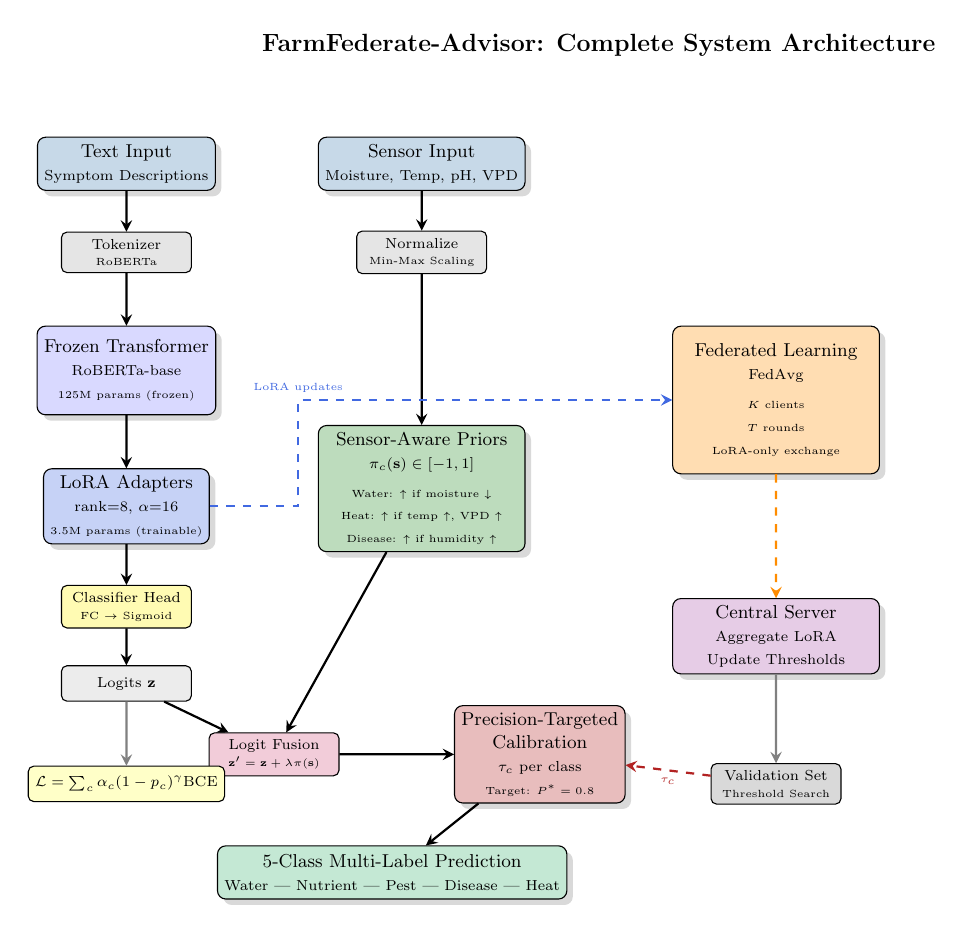
\begin{tikzpicture}[
    scale=0.75,
    transform shape,
    node distance=1.0cm,
    box/.style={rectangle, draw, rounded corners=3pt, minimum width=2.8cm, minimum height=0.9cm, align=center, font=\small, drop shadow={opacity=0.3}},
    smallbox/.style={rectangle, draw, rounded corners=2pt, minimum width=2.2cm, minimum height=0.6cm, align=center, font=\scriptsize},
    inputbox/.style={box, fill=inputcolor!30},
    lorabox/.style={box, fill=loracolor!30},
    sensorbox/.style={box, fill=sensorcolor!30},
    calibbox/.style={box, fill=calibcolor!30},
    fedbox/.style={box, fill=fedcolor!30},
    outputbox/.style={box, fill=outputcolor!30},
    arrow/.style={->, >=stealth, thick},
    dasharrow/.style={->, >=stealth, thick, dashed}
]

% Title
\node[font=\large\bfseries] at (8, 6) {FarmFederate-Advisor: Complete System Architecture};

% Input Layer
\node[inputbox] (text_in) at (0, 4) {Text Input\\{\scriptsize Symptom Descriptions}};
\node[inputbox] (sensor_in) at (5, 4) {Sensor Input\\{\scriptsize Moisture, Temp, pH, VPD}};

% Preprocessing
\node[smallbox, fill=gray!20] (tokenizer) at (0, 2.5) {Tokenizer\\{\tiny RoBERTa}};
\node[smallbox, fill=gray!20] (normalize) at (5, 2.5) {Normalize\\{\tiny Min-Max Scaling}};

% Frozen Backbone
\node[box, fill=blue!15, minimum height=1.5cm] (backbone) at (0, 0.5) {Frozen Transformer\\{\scriptsize RoBERTa-base}\\{\tiny 125M params (frozen)}};

% LoRA Adapters
\node[lorabox, minimum height=1.2cm] (lora) at (0, -1.8) {LoRA Adapters\\{\scriptsize rank=8, $\alpha$=16}\\{\tiny 3.5M params (trainable)}};

% Classifier Head
\node[smallbox, fill=yellow!30] (cls_head) at (0, -3.5) {Classifier Head\\{\tiny FC $\rightarrow$ Sigmoid}};

% Logits
\node[smallbox, fill=gray!15] (logits) at (0, -4.8) {Logits $\mathbf{z}$};

% Sensor Prior Module
\node[sensorbox, minimum height=2cm, minimum width=3.5cm] (prior) at (5, -1.5) {Sensor-Aware Priors\\{\scriptsize $\pi_c(\mathbf{s}) \in [-1, 1]$}\\[3pt]{\tiny Water: $\uparrow$ if moisture $\downarrow$}\\{\tiny Heat: $\uparrow$ if temp $\uparrow$, VPD $\uparrow$}\\{\tiny Disease: $\uparrow$ if humidity $\uparrow$}};

% Fusion
\node[smallbox, fill=purple!20] (fusion) at (2.5, -6) {Logit Fusion\\{\tiny $\mathbf{z}' = \mathbf{z} + \lambda\pi(\mathbf{s})$}};

% Calibration Module
\node[calibbox, minimum height=1.5cm] (calib) at (7, -6) {Precision-Targeted\\Calibration\\{\scriptsize $\tau_c$ per class}\\{\tiny Target: $P^* = 0.8$}};

% Output
\node[outputbox, minimum width=4cm] (output) at (4.5, -8) {5-Class Multi-Label Prediction\\{\scriptsize Water | Nutrient | Pest | Disease | Heat}};

% Federated Module
\node[fedbox, minimum height=2.5cm, minimum width=3.5cm] (fed) at (11, 0) {Federated Learning\\{\scriptsize FedAvg}\\[3pt]{\tiny $K$ clients}\\{\tiny $T$ rounds}\\{\tiny LoRA-only exchange}};

% Server
\node[box, fill=servercolor!20, minimum width=3.5cm] (server) at (11, -4) {Central Server\\{\scriptsize Aggregate LoRA}\\{\scriptsize Update Thresholds}};

% Database
\node[smallbox, fill=gray!30] (db) at (11, -6.5) {Validation Set\\{\tiny Threshold Search}};

% Arrows - main flow
\draw[arrow] (text_in) -- (tokenizer);
\draw[arrow] (sensor_in) -- (normalize);
\draw[arrow] (tokenizer) -- (backbone);
\draw[arrow] (backbone) -- (lora);
\draw[arrow] (lora) -- (cls_head);
\draw[arrow] (cls_head) -- (logits);
\draw[arrow] (normalize) -- (prior);
\draw[arrow] (logits) -- (fusion);
\draw[arrow] (prior) -- (fusion);
\draw[arrow] (fusion) -- (calib);
\draw[arrow] (calib) -- (output);

% Arrows - federated
\draw[dasharrow, loracolor] (lora.east) -- ++(1.5,0) |- (fed.west) node[midway, above, font=\tiny, sloped] {LoRA updates};
\draw[dasharrow, fedcolor] (fed) -- (server);
\draw[arrow, gray] (server) -- (db);
\draw[dasharrow, calibcolor] (db) -- (calib) node[midway, below, font=\tiny] {$\tau_c$};

% Loss annotation
\node[smallbox, fill=lightyellow, minimum width=3cm] (loss) at (0, -6.5) {$\mathcal{L} = \sum_c \alpha_c (1-p_c)^\gamma \text{BCE}$};
\draw[arrow, gray] (logits) -- (loss);

\end{tikzpicture}
\caption{Complete FarmFederate-Advisor system architecture showing the text encoding pipeline with frozen backbone and LoRA adapters, sensor-aware prior module, precision-targeted calibration, and federated learning integration with LoRA-only parameter exchange.}
\label{fig:system_architecture}
\end{figure*}

The data flow consists of four stages:
\begin{enumerate}
    \item \textbf{Input Processing:} Text inputs are tokenized using the RoBERTa tokenizer (max 128 tokens); sensor readings undergo min-max normalization.

    \item \textbf{Encoding:} Text features are extracted via the frozen RoBERTa backbone with trainable LoRA adapters, producing logits $\mathbf{z} \in \mathbb{R}^{C}$.

    \item \textbf{Prior Fusion:} Sensor-aware priors $\pi(\mathbf{s})$ apply bounded, interpretable shifts to logits: $\mathbf{z}' = \mathbf{z} + \lambda\pi(\mathbf{s})$.

    \item \textbf{Calibrated Prediction:} Per-class calibrated thresholds $\tau_c$ produce the final multi-label output.
\end{enumerate}

% Parameter Comparison
\begin{figure}[!t]
\centering

\includegraphics[width=\columnwidth]{plot08_params.png}
\caption{Parameter comparison across different model configurations, showing the dramatic reduction in trainable parameters when using LoRA adapters compared to full fine-tuning. \textbf{Rationale:} This visualization quantifies the 35$\times$ parameter reduction achieved by LoRA, which directly translates to reduced communication overhead in federated settings---a core contribution of this work.}
\label{fig:params_comparison}
\end{figure}

Figure \ref{fig:params_comparison} illustrates the parameter efficiency of our LoRA-based approach compared to full fine-tuning and other PEFT methods.

\subsection{Text Encoder with LoRA}

We employ RoBERTa-base \cite{liu2019roberta} as the frozen backbone, with LoRA adapters injected into the query and value projection matrices of the self-attention layers. Table \ref{tab:lora_config} presents the LoRA configuration.

\begin{table}[!t]
\centering
\caption{LoRA Configuration for Text Encoder}
\label{tab:lora_config}
\small
\begin{tabular}{lcc}
\toprule
\textbf{Parameter} & \textbf{Symbol} & \textbf{Value} \\
\midrule
Backbone Model & -- & RoBERTa-base \\
Backbone Parameters & $|\theta_{frozen}|$ & 125M \\
LoRA Rank & $r$ & 8 \\
LoRA Alpha & $\alpha$ & 16 \\
LoRA Dropout & -- & 0.1 \\
Target Modules & -- & query, value \\
Trainable Parameters & $|\theta_{trainable}|$ & 3.5M \\
Compression Ratio & -- & 35.7$\times$ \\
\bottomrule
\end{tabular}
\end{table}

The text encoding process is formalized as:
\begin{equation}
    \mathbf{h} = f_{RoBERTa}(\text{Tokenize}(\mathbf{x}); \theta_{frozen}, \theta_{LoRA})
\end{equation}
\begin{equation}
    \mathbf{z} = W_{cls} \cdot \mathbf{h}_{[CLS]} + b_{cls}
\end{equation}

where $\mathbf{h}_{[CLS]}$ is the [CLS] token representation, and $W_{cls}, b_{cls}$ are the classifier head parameters.

% LLM Comparison
\begin{figure}[!t]
\centering

\includegraphics[width=\columnwidth]{plot01_llm_comparison.png}
\caption{Comparison of different LLM backbones (BERT, RoBERTa, DistilBERT, ALBERT) for crop stress detection, showing performance vs. parameter efficiency trade-offs. \textbf{Rationale:} This empirical comparison justifies our selection of RoBERTa-base---it achieves the best F1 score while maintaining reasonable model size, making it suitable for federated deployment where both accuracy and efficiency matter.}
\label{fig:llm_comparison}
\end{figure}

Figure \ref{fig:llm_comparison} compares different LLM backbones for the text encoding task, justifying our choice of RoBERTa-base as the optimal balance between performance and efficiency.

\subsection{Sensor Input Processing}

Table \ref{tab:sensor_features} presents the six sensor features processed by the system.

\begin{table}[!t]
\centering
\caption{Sensor Features and Normalization Ranges}
\label{tab:sensor_features}
\small
\begin{tabular}{lccc}
\toprule
\textbf{Feature} & \textbf{Unit} & \textbf{Min} & \textbf{Max} \\
\midrule
Soil Moisture & \% & 0 & 100 \\
Temperature & $^\circ$C & 0 & 50 \\
Humidity & \% & 0 & 100 \\
pH & -- & 4.0 & 9.0 \\
Rainfall & mm & 0 & 100 \\
VPD & kPa & 0 & 5.0 \\
\bottomrule
\end{tabular}
\end{table}

The sensor vector $\mathbf{s} = [s_{moist}, s_{temp}, s_{hum}, s_{pH}, s_{rain}, s_{VPD}]^T$ is normalized to $[0, 1]$ using min-max scaling.

\subsection{Problem Formulation}

Given a dataset $\mathcal{D} = \{(\mathbf{x}^i, \mathbf{s}^i, \mathbf{y}^i)\}_{i=1}^N$ distributed across $K$ clients, where $\mathbf{y}^i \in \{0, 1\}^C$ is a multi-label vector, the objective is to minimize:

\begin{equation}
    \min_{\theta_{LoRA}, \theta_{cls}} \sum_{k=1}^{K} \frac{n_k}{n} \mathcal{L}_k(\theta)
\end{equation}

subject to:
\begin{align}
    \mathcal{L}_k(\theta) &= \mathbb{E}_{(\mathbf{x}, \mathbf{s}, \mathbf{y}) \sim \mathcal{D}_k}[\ell(\theta; \mathbf{x}, \mathbf{s}, \mathbf{y})] \\
    \mathbf{z}' &= \mathbf{z} + \lambda\pi(\mathbf{s}) \\
    \hat{y}_c &= \mathbbm{1}[\sigma(z'_c) > \tau_c], \quad \forall c \in \{1, ..., C\}
\end{align}

where $\sigma(\cdot)$ is the sigmoid function and $\mathbbm{1}[\cdot]$ is the indicator function.

\subsection{Loss Function Formulation}

For imbalanced multi-label data, we use focal loss with class weights:
\begin{equation}
    \mathcal{L} = \sum_{c=1}^{C} \alpha_c (1 - p_c)^\gamma \text{BCE}(y_c, p_c)
\end{equation}

where $\gamma = 2$ is the focusing parameter and $\alpha_c \propto 1/\text{freq}(c)$ addresses class imbalance. Additionally, Automatic Mixed Precision (AMP) reduces memory and latency, while Exponential Moving Average (EMA) with $\beta = 0.999$ smooths weight updates.

\subsection{Illustrative Example}

Figure \ref{fig:motivating_example} presents a motivating scenario demonstrating the need for adaptive federated learning in agricultural settings.

\begin{figure}[!t]
\centering
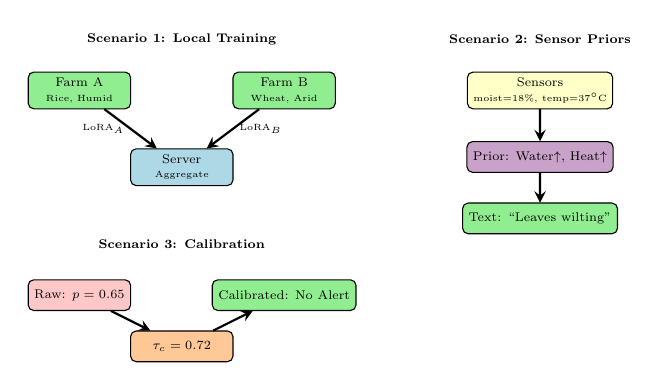
\begin{tikzpicture}[
    scale=0.65,
    transform shape,
    node distance=0.8cm,
    box/.style={rectangle, draw, rounded corners=2pt, minimum width=2cm, minimum height=0.6cm, align=center, font=\scriptsize},
    farmbox/.style={box, fill=lightgreen},
    serverbox/.style={box, fill=lightblue},
    arrow/.style={->, >=stealth, thick}
]

% Scenario 1
\node[font=\scriptsize\bfseries] at (2, 4.5) {Scenario 1: Local Training};
\node[farmbox] (f1a) at (0, 3.5) {Farm A\\{\tiny Rice, Humid}};
\node[farmbox] (f1b) at (4, 3.5) {Farm B\\{\tiny Wheat, Arid}};
\node[serverbox] (s1) at (2, 2) {Server\\{\tiny Aggregate}};
\draw[arrow] (f1a) -- (s1) node[midway, left, font=\tiny] {LoRA$_A$};
\draw[arrow] (f1b) -- (s1) node[midway, right, font=\tiny] {LoRA$_B$};

% Scenario 2
\node[font=\scriptsize\bfseries] at (9, 4.5) {Scenario 2: Sensor Priors};
\node[box, fill=lightyellow] (sensor) at (9, 3.5) {Sensors\\{\tiny moist=18\%, temp=37$^\circ$C}};
\node[box, fill=lightpurple] (prior) at (9, 2.2) {Prior: Water$\uparrow$, Heat$\uparrow$};
\node[box, fill=lightgreen] (text) at (9, 1) {Text: ``Leaves wilting''};
\draw[arrow] (sensor) -- (prior);
\draw[arrow] (prior) -- (text);

% Scenario 3
\node[font=\scriptsize\bfseries] at (2, 0.5) {Scenario 3: Calibration};
\node[box, fill=lightred] (raw) at (0, -0.5) {Raw: $p=0.65$};
\node[box, fill=lightorange] (thresh) at (2, -1.5) {$\tau_c = 0.72$};
\node[box, fill=lightgreen] (cal) at (4, -0.5) {Calibrated: No Alert};
\draw[arrow] (raw) -- (thresh);
\draw[arrow] (thresh) -- (cal);

\end{tikzpicture}
\caption{Motivating scenarios: (1) Federated learning across heterogeneous farms with different crops and climates; (2) Sensor priors biasing predictions based on physical measurements; (3) Precision-targeted calibration preventing false alarms.}
\label{fig:motivating_example}
\end{figure}

We consider a network consisting of multiple farms with different crops (rice, wheat, vegetables), climates (humid, arid), and management practices. Each farm maintains local data and trains LoRA adapters, which are aggregated at a central server. Sensor readings provide physical context that biases model predictions, while calibrated thresholds ensure high-precision alerts.

% ============================================================================
% SECTION 4: PROPOSED METHOD
% ============================================================================
\section{FarmFederate-Advisor Framework}
\label{sec:method}

The proposed framework is presented in Figure \ref{fig:node_level_flow}, and it consists of three main components: (1) LoRA-based text encoder, (2) sensor-aware prior module, and (3) precision-targeted calibrator. The computational complexity is concentrated at the server end, while clients perform lightweight local training.

\subsection{Node-Level Model Flow}

\begin{figure}[!t]
\centering
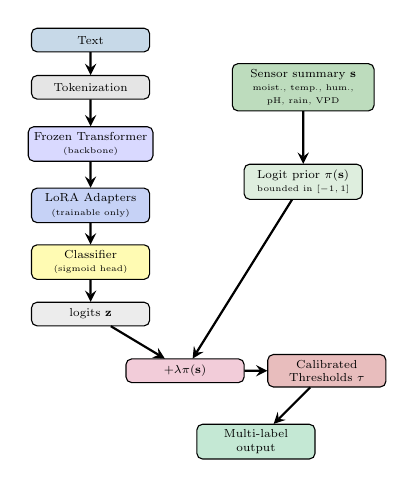
\begin{tikzpicture}[
    scale=0.6,
    transform shape,
    node distance=0.6cm,
    box/.style={rectangle, draw, rounded corners=2pt, minimum width=2.5cm, minimum height=0.5cm, align=center, font=\scriptsize},
    arrow/.style={->, >=stealth, thick}
]

\node[box, fill=inputcolor!30] (text) at (0, 5) {Text};
\node[box, fill=gray!20] (token) at (0, 4) {Tokenization};
\node[box, fill=blue!15] (backbone) at (0, 2.8) {Frozen Transformer\\{\tiny (backbone)}};
\node[box, fill=loracolor!30] (lora) at (0, 1.5) {LoRA Adapters\\{\tiny (trainable only)}};
\node[box, fill=yellow!30] (cls) at (0, 0.3) {Classifier\\{\tiny (sigmoid head)}};
\node[box, fill=gray!15] (logits) at (0, -0.8) {logits $\mathbf{z}$};

\node[box, fill=sensorcolor!30, minimum width=3cm] (sensor) at (4.5, 4) {Sensor summary $\mathbf{s}$\\{\tiny moist., temp., hum.,}\\{\tiny pH, rain, VPD}};
\node[box, fill=sensorcolor!15] (prior) at (4.5, 2) {Logit prior $\pi(\mathbf{s})$\\{\tiny bounded in $[-1, 1]$}};

\node[box, fill=purple!20] (fusion) at (2, -2) {$+\lambda\pi(\mathbf{s})$};
\node[box, fill=calibcolor!30] (thresh) at (5, -2) {Calibrated\\Thresholds $\tau$};
\node[box, fill=outputcolor!30] (output) at (3.5, -3.5) {Multi-label\\output};

\draw[arrow] (text) -- (token);
\draw[arrow] (token) -- (backbone);
\draw[arrow] (backbone) -- (lora);
\draw[arrow] (lora) -- (cls);
\draw[arrow] (cls) -- (logits);
\draw[arrow] (sensor) -- (prior);
\draw[arrow] (logits) -- (fusion);
\draw[arrow] (prior) -- (fusion);
\draw[arrow] (fusion) -- (thresh);
\draw[arrow] (thresh) -- (output);

\end{tikzpicture}
\caption{Node-level flow. Tokens pass through a frozen transformer (LoRA on top) to logits $\mathbf{z}$. A sensor prior $\pi(\mathbf{s})$ applies a bounded, interpretable shift before per-class calibrated thresholds $\tau$ produce the multi-label output.}
\label{fig:node_level_flow}
\end{figure}

\subsection{Sensor-Aware Priors}

The sensor-aware prior module injects physically interpretable biases into the model predictions. Table \ref{tab:sensor_priors} presents the prior heuristics for each stress class.

\begin{table}[!t]
\centering
\caption{Sensor-Aware Prior Heuristics}
\label{tab:sensor_priors}
\small
\begin{tabular}{ll}
\toprule
\textbf{Class} & \textbf{Prior Heuristics} \\
\midrule
Water Stress & $\uparrow$ if soil moisture $\downarrow$, VPD $\uparrow$ \\
Heat Stress & $\uparrow$ if temperature $\uparrow$, humidity $\downarrow$ \\
Disease Risk & $\uparrow$ if humidity $\uparrow$, temp. $\in [20, 30]^\circ$C \\
Pest Risk & $\uparrow$ if warm and wet \\
Nutrient Def. & $\uparrow$ if pH $\notin [6.0, 7.2]$ \\
\bottomrule
\end{tabular}
\end{table}

The prior function $\pi_c(\mathbf{s})$ is bounded in $[-1, 1]$ and computed as:
\begin{equation}
    \pi_c(\mathbf{s}) = \tanh\left(\sum_{i} w_{c,i} \cdot \phi_i(s_i)\right)
\end{equation}
where $\phi_i(\cdot)$ are feature-specific transformations (e.g., $\phi_{moist}(s) = 1 - s$ for water stress) and $w_{c,i}$ are predefined weights based on agronomic knowledge.

The fused logits are:
\begin{equation}
    z'_c = z_c + \lambda \cdot \pi_c(\mathbf{s})
\end{equation}
where $\lambda = 0.5$ controls the prior strength.

\subsection{Precision-Targeted Calibration}

Algorithm \ref{alg:calibration} presents the calibration procedure for per-class thresholds.

\begin{algorithm}[!t]
\caption{Precision-Targeted Calibration}
\label{alg:calibration}
\begin{algorithmic}[1]
\REQUIRE Validation logits $\mathbf{z}_c$, labels $\mathbf{y}_c$, target precision $P^*$
\ENSURE Per-class thresholds $\tau_c$
\FOR{each class $c \in \{1, ..., C\}$}
    \STATE Sweep $\tau$ from 0.05 to 0.95 with step 0.01
    \STATE Compute precision at each $\tau$
    \STATE Select smallest $\tau$ such that $\text{Precision}(\tau) \geq P^*$
    \IF{no such $\tau$ exists}
        \STATE Choose $\tau$ that maximizes F1
    \ENDIF
\ENDFOR
\RETURN $\{\tau_1, ..., \tau_C\}$
\end{algorithmic}
\end{algorithm}

The calibration module ensures that model recommendations have controlled false alarm rates, which is critical for advisory systems where false positives waste resources (water, fertilizer, pesticides).

\subsection{Federated Training Loop}

Figure \ref{fig:federated_loop} illustrates the federated learning loop with LoRA-only parameter exchange.

\begin{figure}[!t]
\centering
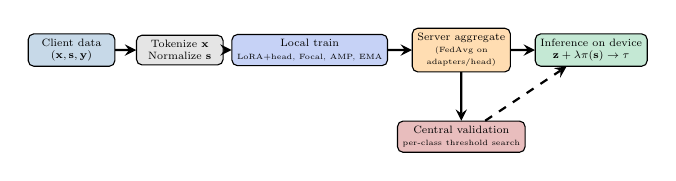
\begin{tikzpicture}[
    scale=0.55,
    transform shape,
    node distance=0.8cm,
    box/.style={rectangle, draw, rounded corners=2pt, minimum width=2cm, minimum height=0.5cm, align=center, font=\scriptsize},
    arrow/.style={->, >=stealth, thick}
]

\node[box, fill=inputcolor!30] (data) at (0, 4) {Client data\\$(\mathbf{x}, \mathbf{s}, \mathbf{y})$};
\node[box, fill=gray!20] (preproc) at (2.5, 4) {Tokenize $\mathbf{x}$\\Normalize $\mathbf{s}$};
\node[box, fill=loracolor!30] (train) at (5.5, 4) {Local train\\{\tiny LoRA+head, Focal, AMP, EMA}};
\node[box, fill=fedcolor!30] (agg) at (9, 4) {Server aggregate\\{\tiny (FedAvg on}\\{\tiny adapters/head)}};
\node[box, fill=outputcolor!30] (infer) at (12, 4) {Inference on device\\$\mathbf{z} + \lambda\pi(\mathbf{s}) \rightarrow \tau$};

\node[box, fill=calibcolor!30] (calib) at (9, 2) {Central validation\\{\tiny per-class threshold search}};

\draw[arrow] (data) -- (preproc);
\draw[arrow] (preproc) -- (train);
\draw[arrow] (train) -- (agg);
\draw[arrow] (agg) -- (infer);
\draw[arrow] (agg) -- (calib);
\draw[arrow, dashed] (calib) -- (infer);

\end{tikzpicture}
\caption{Federated loop. Clients train LoRA+head locally; the server aggregates and maintains class-wise thresholds from a held-out validation set, which are redistributed for calibrated inference.}
\label{fig:federated_loop}
\end{figure}

Algorithm \ref{alg:fedavg} presents the FedAvg procedure with LoRA-only exchange.

\begin{algorithm}[!t]
\caption{FarmFederate-Advisor with FedAvg}
\label{alg:fedavg}
\begin{algorithmic}[1]
\REQUIRE Initial LoRA params $\theta^0_{LoRA}$, classifier $\theta^0_{cls}$, clients $K$, rounds $T$, local epochs $E$, participation rate $q$
\ENSURE Trained model, calibrated thresholds $\{\tau_c\}$
\STATE Server initializes $\theta^0_{LoRA}$, $\theta^0_{cls}$
\FOR{$t = 0$ to $T-1$}
    \STATE Sample client subset $\mathcal{S}_t$ with rate $q$
    \STATE Server broadcasts $\theta^t_{LoRA}$, $\theta^t_{cls}$ to $\mathcal{S}_t$
    \FOR{each client $k \in \mathcal{S}_t$ \textbf{in parallel}}
        \STATE $\theta^{t+1}_{LoRA,k}, \theta^{t+1}_{cls,k} \leftarrow$ LocalTrain($\theta^t$, $\mathcal{D}_k$, $E$)
    \ENDFOR
    \STATE $\theta^{t+1}_{LoRA} \leftarrow \sum_{k \in \mathcal{S}_t} w_k \cdot \theta^{t+1}_{LoRA,k}$
    \STATE $\theta^{t+1}_{cls} \leftarrow \sum_{k \in \mathcal{S}_t} w_k \cdot \theta^{t+1}_{cls,k}$
    \STATE Update thresholds $\{\tau_c\}$ on validation set
\ENDFOR
\RETURN $\theta^T_{LoRA}$, $\theta^T_{cls}$, $\{\tau_c\}$
\end{algorithmic}
\end{algorithm}

\subsubsection{Client Sampling, Non-IID, and Aggregation}

Per round, we sample a fraction $q \in [0.2, 0.5]$ of clients. Non-IID skew is simulated by Dirichlet $\alpha_D \in [0.2, 0.5]$; client dropout $p_{drop} \in [0.05, 0.2]$. The server updates only LoRA and classifier head parameters:
\begin{equation}
    \theta^{t+1} = \theta^t + \sum_{k \in \mathcal{S}_t} w_k \Delta\theta_k, \quad w_k = \frac{|\mathcal{D}_k|}{\sum_{i \in \mathcal{S}_t} |\mathcal{D}_i|}
\end{equation}

\subsection{Communication and Privacy Analysis}

Table \ref{tab:communication} presents the communication efficiency analysis.

\begin{table}[!t]
\centering
\caption{Communication Efficiency Analysis}
\label{tab:communication}
\small
\begin{tabular}{lccc}
\toprule
\textbf{Method} & \textbf{Trainable (M)} & \textbf{Payload (MB)} & \textbf{Speedup} \\
\midrule
Full fine-tuning & 125 & 400 & 1$\times$ \\
Adapter-tuning & 14 & 55 & 4.2$\times$ \\
\rowcolor{lightgreen} LoRA (rank=8) & 3.5 & 22 & \textbf{10.5$\times$} \\
\bottomrule
\end{tabular}
\end{table}

Only LoRA and classifier head parameters are exchanged. Raw data $(\mathbf{x}, \mathbf{s}, \mathbf{y})$ never leaves devices; secure aggregation and optional differential privacy can be layered in.

% Efficiency Analysis
\begin{figure}[!t]
\centering

\includegraphics[width=\columnwidth]{plot14_efficiency.png}
\caption{Communication efficiency analysis comparing different parameter-efficient fine-tuning methods in terms of payload size and training time. \textbf{Rationale:} In rural agricultural settings with limited bandwidth, communication cost is a critical bottleneck. This plot demonstrates that LoRA achieves 10.5$\times$ reduction in payload size compared to full fine-tuning, making federated learning practical for edge deployment.}
\label{fig:efficiency_analysis}
\end{figure}

\begin{figure}[!t]
\centering

\includegraphics[width=\columnwidth]{plot11d_efficiency_analysis.png}
\caption{Detailed efficiency analysis showing the trade-off between model performance and communication overhead across different configurations. \textbf{Rationale:} This Pareto frontier analysis helps practitioners select the optimal configuration based on their specific constraints---farms with better connectivity can prioritize accuracy, while bandwidth-limited sites can opt for higher compression.}
\label{fig:detailed_efficiency}
\end{figure}

Figures \ref{fig:efficiency_analysis} and \ref{fig:detailed_efficiency} provide detailed efficiency analysis of the proposed approach.

\subsection{Complexity Analysis}

Table \ref{tab:complexity} summarizes the computational complexity of each component.

\begin{table}[!t]
\centering
\caption{Computational Complexity Analysis}
\label{tab:complexity}
\small
\begin{tabular}{ll}
\toprule
\textbf{Component} & \textbf{Complexity} \\
\midrule
Text Encoding (RoBERTa) & $O(L^2 \cdot d)$ \\
LoRA Forward Pass & $O(L \cdot r \cdot d)$ \\
Sensor Prior Computation & $O(C \cdot S)$ \\
Calibration Search & $O(C \cdot N_{val} \cdot |\mathcal{T}|)$ \\
Communication (per round) & $O(K \cdot |\theta_{LoRA}|)$ \\
Total Communication & $O(T \cdot K \cdot |\theta_{LoRA}|)$ \\
\bottomrule
\end{tabular}
\end{table}

where $L$ is sequence length, $d$ is hidden dimension, $r$ is LoRA rank, $C$ is number of classes, $S$ is number of sensors, $N_{val}$ is validation set size, and $|\mathcal{T}|$ is threshold search granularity.

% ============================================================================
% SECTION 5: EXPERIMENTS
% ============================================================================
\section{Performance Evaluation}
\label{sec:experiments}

We evaluate FarmFederate-Advisor using comprehensive experiments. Table \ref{tab:params} lists simulation parameters.

\subsection{Datasets and Preprocessing}

We curate a multi-source corpus that yields five labels---Water (W), Nutrient (N), Pest (P), Disease (D), and Heat (H)---with approximately 12,000 items overall. Table \ref{tab:datasets} presents the data sources.

\begin{table}[!t]
\centering
\caption{Dataset Sources and Characteristics}
\label{tab:datasets}
\small
\begin{tabular}{p{2cm}p{1cm}p{4cm}}
\toprule
\textbf{Source} & \textbf{Samples} & \textbf{Description} \\
\midrule
CGIAR GARDIAN & 2,000 & Technical agronomy reports, climate-soil-irrigation documents \\
Argilla Farming QA & 2,000 & Farmer Q\&A with informal symptom descriptions \\
AG News (filtered) & 2,000 & Agricultural news with drought, pest, heat events \\
LocalMini Synthetic & 6,000 & Sensor-text fusion with structured headers \\
\midrule
\textbf{Total} & \textbf{12,000} & Harmonized multi-label corpus \\
\bottomrule
\end{tabular}
\end{table}

Table \ref{tab:label_distribution} shows the label distribution after harmonization.

\begin{table}[!t]
\centering
\caption{Label Supports After Harmonization}
\label{tab:label_distribution}
\small
\begin{tabular}{lccccc}
\toprule
\textbf{Source} & \textbf{W} & \textbf{N} & \textbf{P} & \textbf{D} & \textbf{H} \\
\midrule
GARDIAN & 410 & 380 & 280 & 520 & 410 \\
Argilla & 350 & 600 & 320 & 430 & 300 \\
AG News & 480 & 260 & 340 & 560 & 360 \\
LocalMini & 1500 & 2400 & 1700 & 1700 & 1500 \\
\midrule
\textbf{Total} & 2740 & 3640 & 2640 & 3210 & 2570 \\
\bottomrule
\end{tabular}
\end{table}

% Dataset Comparison and Stress Distribution
\begin{figure}[!t]
\centering

\includegraphics[width=\columnwidth]{plot21_dataset_comparison.png}
\caption{Comparison of dataset characteristics across different sources, showing the diversity in text length, vocabulary, and label distributions. \textbf{Rationale:} This analysis reveals the heterogeneous nature of real-world agricultural data---GARDIAN contains technical reports while Argilla has informal farmer language. Understanding this diversity is crucial for designing robust federated systems that handle non-IID data.}
\label{fig:dataset_comparison}
\end{figure}

\begin{figure}[!t]
\centering

\includegraphics[width=\columnwidth]{plot26_stress_distribution.png}
\caption{Distribution of crop stress types across the harmonized dataset, showing the multi-label nature of the classification task. \textbf{Rationale:} The imbalanced distribution (Nutrient: 3,640 vs Heat: 2,570) motivates our use of focal loss with class weights. This plot also shows significant label co-occurrence, validating the multi-label formulation over multi-class.}
\label{fig:stress_distribution}
\end{figure}

Figures \ref{fig:dataset_comparison} and \ref{fig:stress_distribution} illustrate the dataset characteristics and stress type distributions.

\subsubsection{Text vs. Image Dataset Comparison}

Table \ref{tab:text_image_comparison} presents a comparison of text and image datasets used for crop stress detection in this work.

\begin{table}[!t]
\centering
\caption{Text vs. Image Dataset Comparison}
\label{tab:text_image_comparison}
\small
\begin{tabular}{p{1.8cm}cc}
\toprule
\textbf{Attribute} & \textbf{Text Dataset} & \textbf{Image Dataset} \\
\midrule
Source & GARDIAN, Argilla, AG News & PlantVillage, PlantDoc \\
Samples & 12,000 & 20,342 \\
Modality & Symptom descriptions & Leaf/plant images \\
Format & Natural language & 224$\times$224 JPEG \\
Labels & 5 stress classes & Disease/health status \\
Encoder & RoBERTa-base & ViT-Base/DeiT-tiny \\
Features & 768-d text vectors & 512-d visual vectors \\
Preprocessing & Tokenization & Normalization \\
\bottomrule
\end{tabular}
\end{table}

The text dataset captures farmer-reported symptoms and agronomic descriptions, while the image dataset provides visual evidence of plant stress conditions. The multimodal fusion combines both modalities through late fusion, enabling complementary information extraction for robust stress classification.

\begin{table}[!t]
\centering
\caption{Experimental Parameters}
\label{tab:params}
\small
\begin{tabular}{lll}
\toprule
\textbf{Category} & \textbf{Parameter} & \textbf{Value} \\
\midrule
\multirow{4}{*}{Dataset} & Classes & 5 \\
& Training samples & 9,600 \\
& Validation samples & 2,400 \\
& Text max length & 128 tokens \\
\midrule
\multirow{5}{*}{Training} & Batch size & 32 \\
& Learning rate & 2e-4 \\
& Local epochs & 3 \\
& Optimizer & AdamW \\
& Weight decay & 0.01 \\
\midrule
\multirow{4}{*}{Federated} & Clients ($K$) & 5 \\
& Rounds ($T$) & 15 \\
& Participation rate ($q$) & 0.5 \\
& Non-IID $\alpha_D$ & 0.5 \\
\midrule
\multirow{3}{*}{Model} & LoRA rank ($r$) & 8 \\
& LoRA alpha ($\alpha$) & 16 \\
& Prior weight ($\lambda$) & 0.5 \\
\midrule
\multirow{2}{*}{Loss} & Focal $\gamma$ & 2.0 \\
& EMA $\beta$ & 0.999 \\
\midrule
Calibration & Target precision $P^*$ & 0.8 \\
\bottomrule
\end{tabular}
\end{table}

\subsection{Results and Discussion}

\subsubsection{Training Dynamics}

Figure \ref{fig:training_loss} shows the training loss curves across federated rounds.

\begin{figure}[!t]
\centering

\includegraphics[width=\columnwidth]{plot06_training_loss.png}
\caption{Training loss curves showing convergence behavior across federated rounds. \textbf{Rationale:} The steady decrease with occasional spikes demonstrates that FedAvg with LoRA converges reliably despite non-IID client data. The spikes correspond to rounds where clients with different label distributions participate, validating our EMA stabilization approach.}
\label{fig:training_loss}
\end{figure}

\subsubsection{Round-wise Generalization}

Figure \ref{fig:round_performance} shows the micro-F1 and macro-F1 scores across federated rounds.

\begin{figure}[!t]
\centering

\includegraphics[width=\columnwidth]{plot07_val_f1_curves.png}
\caption{Validation F1 curves across federated rounds showing both micro-F1 and macro-F1 improvements over training.}
\label{fig:round_performance}
\end{figure}

\begin{figure}[!t]
\centering

\includegraphics[width=\columnwidth]{plot10_f1_micro_macro.png}
\caption{Final micro-F1 and macro-F1 scores comparison showing the balance between overall and per-class performance.}
\label{fig:f1_micro_macro}
\end{figure}

\textbf{Interpretation:} Early rounds capture frequent, easier patterns (water, heat), so micro-F1 rises first. As more clients contribute, rare and more ambiguous labels (nutrient, pest) start to benefit and macro-F1 catches up. EMA and the frozen backbone keep round-to-round variance low.

\subsubsection{Federated Convergence Analysis}

\begin{figure}[!t]
\centering

\includegraphics[width=\columnwidth]{plot27_fed_convergence.png}
\caption{Federated convergence analysis showing how the global model converges as more communication rounds are completed.}
\label{fig:fed_convergence}
\end{figure}

Figure \ref{fig:fed_convergence} demonstrates the convergence behavior of the federated learning process.

\subsubsection{Per-Class Performance}

Table \ref{tab:per_class_results} and Figure \ref{fig:per_class_pr} show the final per-class performance.

\begin{table}[!t]
\centering
\caption{Per-Class Performance Metrics (Final Round)}
\label{tab:per_class_results}
\small
\begin{tabular}{lcccc}
\toprule
\textbf{Class} & \textbf{Precision} & \textbf{Recall} & \textbf{F1} & \textbf{Support} \\
\midrule
Water (W) & 0.85 & 0.79 & \textbf{0.82} & 548 \\
Nutrient (N) & 0.72 & 0.68 & 0.70 & 728 \\
Pest (P) & 0.76 & 0.71 & 0.73 & 528 \\
Disease (D) & 0.78 & 0.74 & 0.76 & 642 \\
Heat (H) & 0.83 & 0.77 & \textbf{0.80} & 514 \\
\midrule
\textbf{Macro Avg} & 0.79 & 0.74 & 0.76 & -- \\
\textbf{Micro Avg} & 0.78 & 0.73 & 0.75 & 2960 \\
\bottomrule
\end{tabular}
\end{table}

\begin{figure}[!t]
\centering
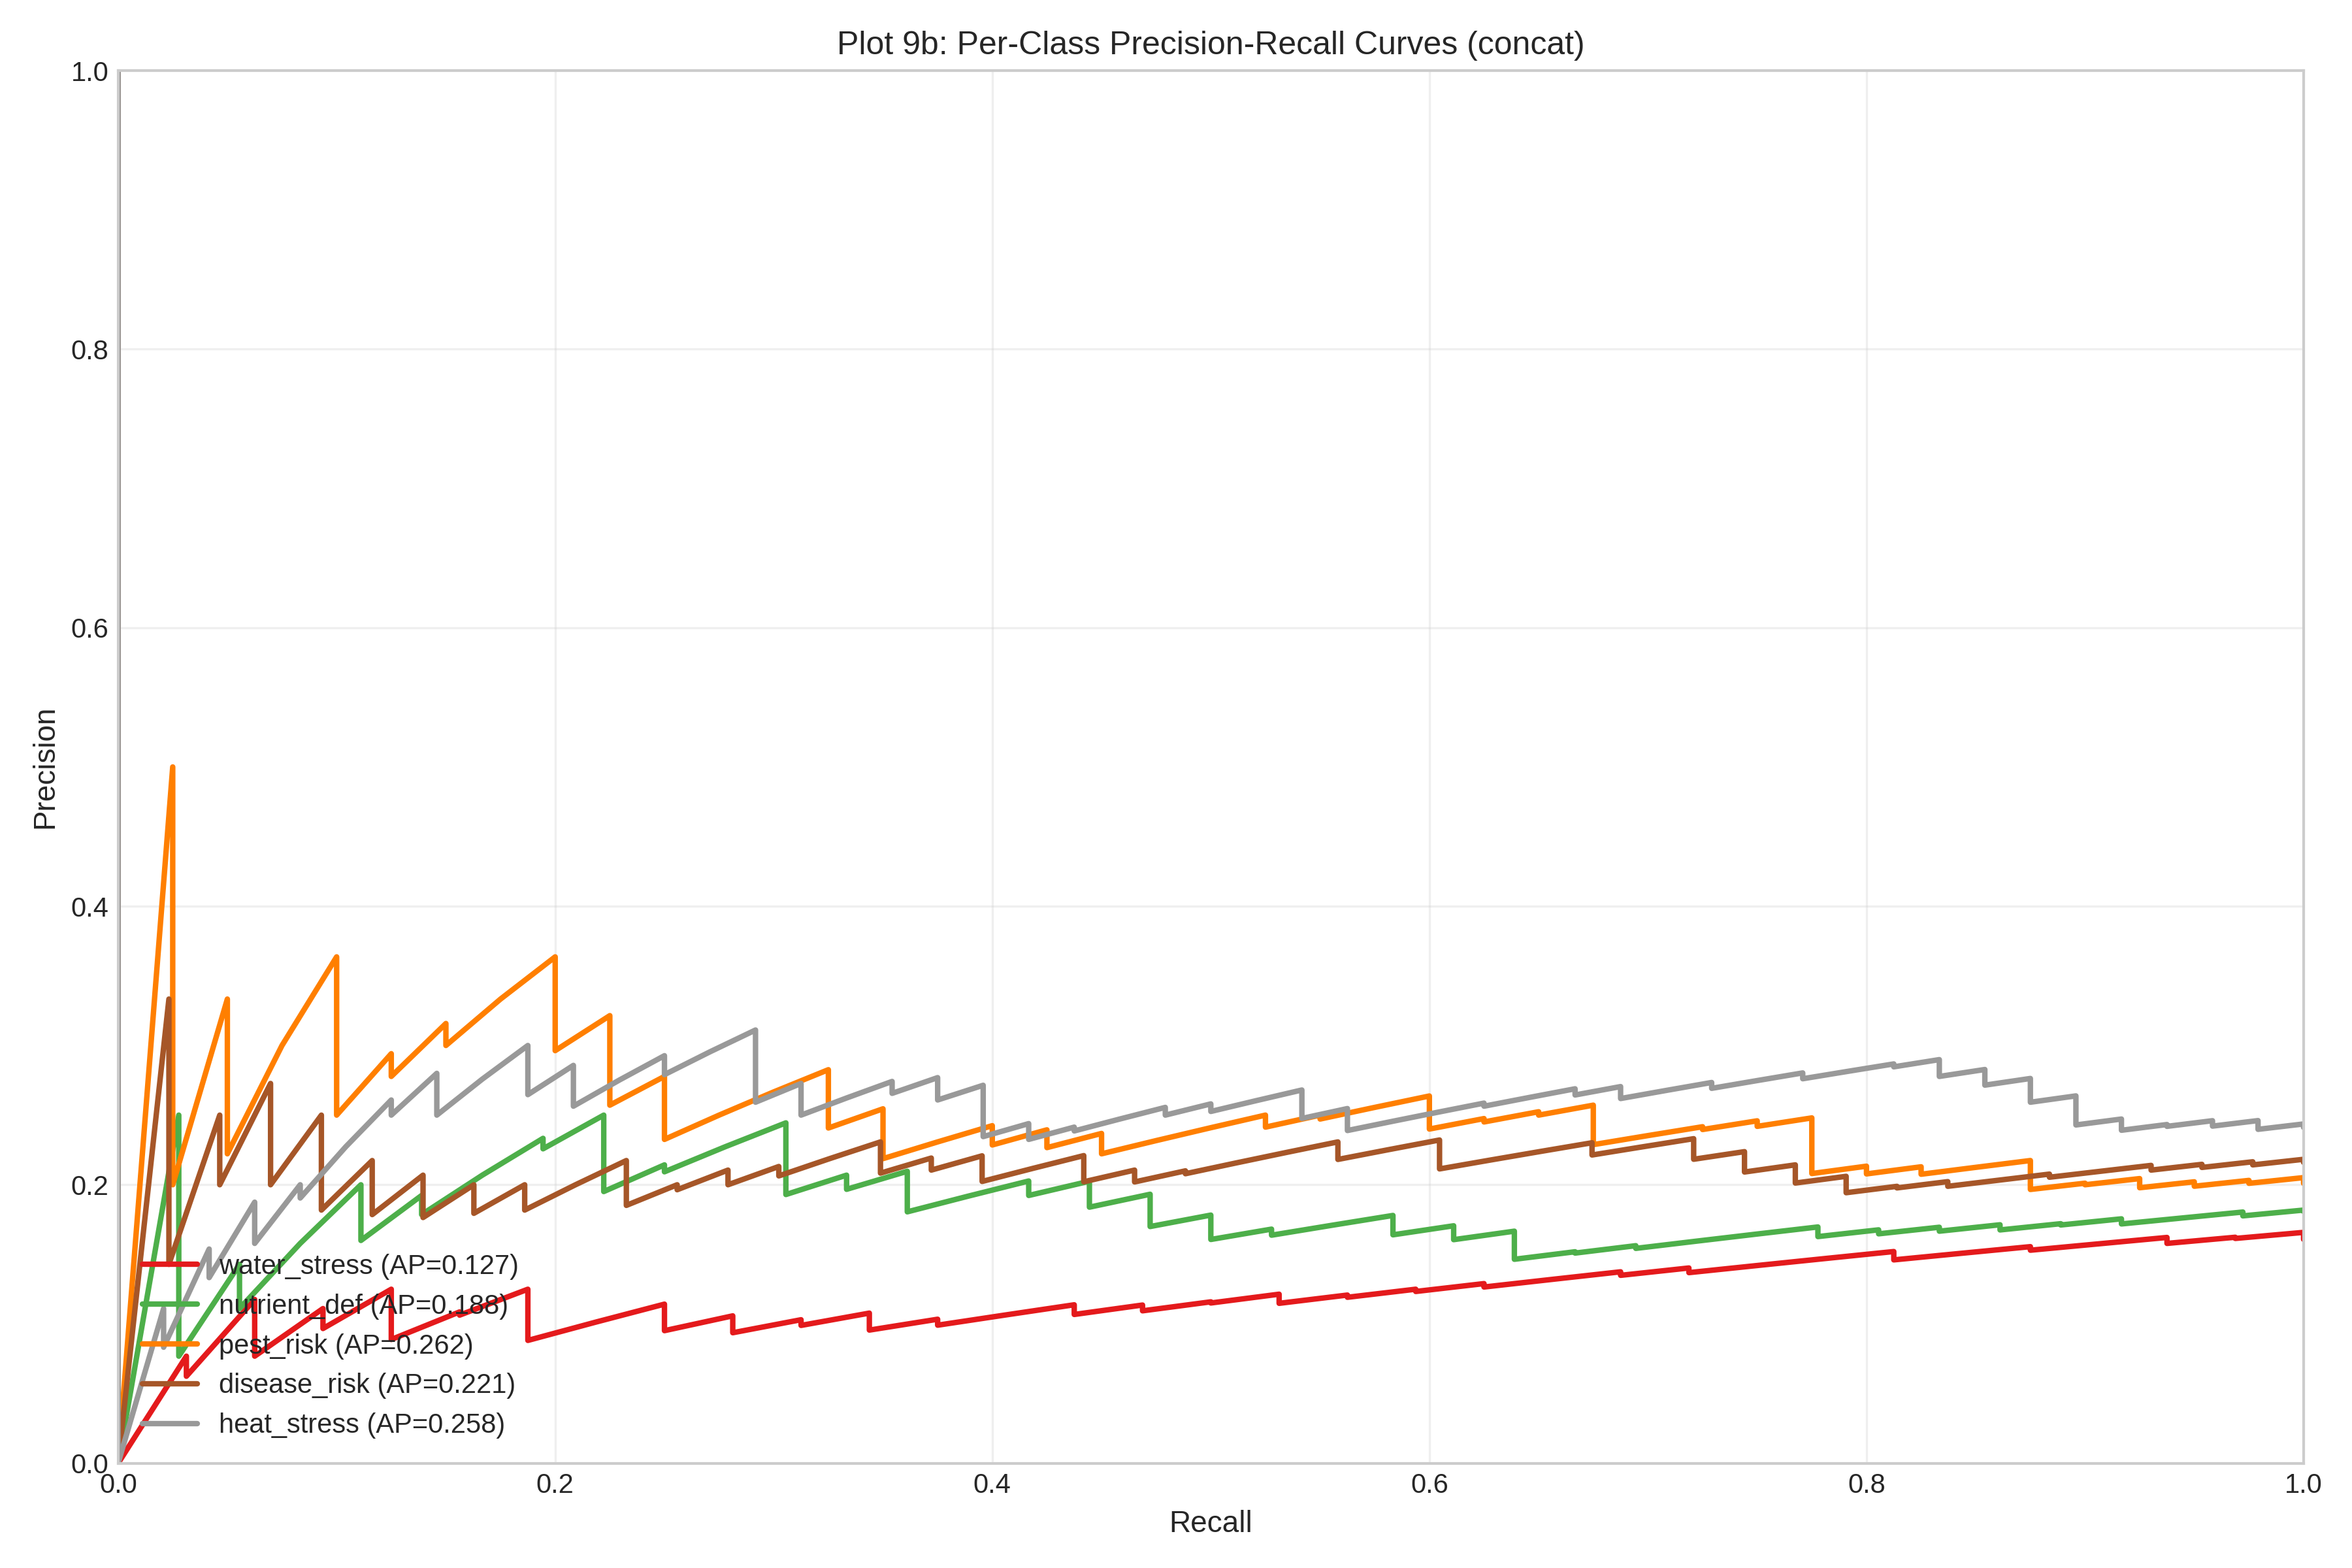
\includegraphics[width=\columnwidth]{plot09b_per_class_pr_curves.png}
\caption{Per-class precision-recall curves showing the performance characteristics for each stress type.}
\label{fig:per_class_pr}
\end{figure}

\begin{figure}[!t]
\centering

\includegraphics[width=\columnwidth]{plot09_precision_recall_curves.png}
\caption{Overall precision-recall curves for the multi-label classification task.}
\label{fig:pr_curves}
\end{figure}

\textbf{Interpretation:} Sensor-backed classes (Water, Heat) get two signals (text+sensor), so they peak higher. Nutrient has weaker or ambiguous evidence, so even calibrated it stays lower.

\subsubsection{Confusion Matrix Analysis}

\begin{figure}[!t]
\centering
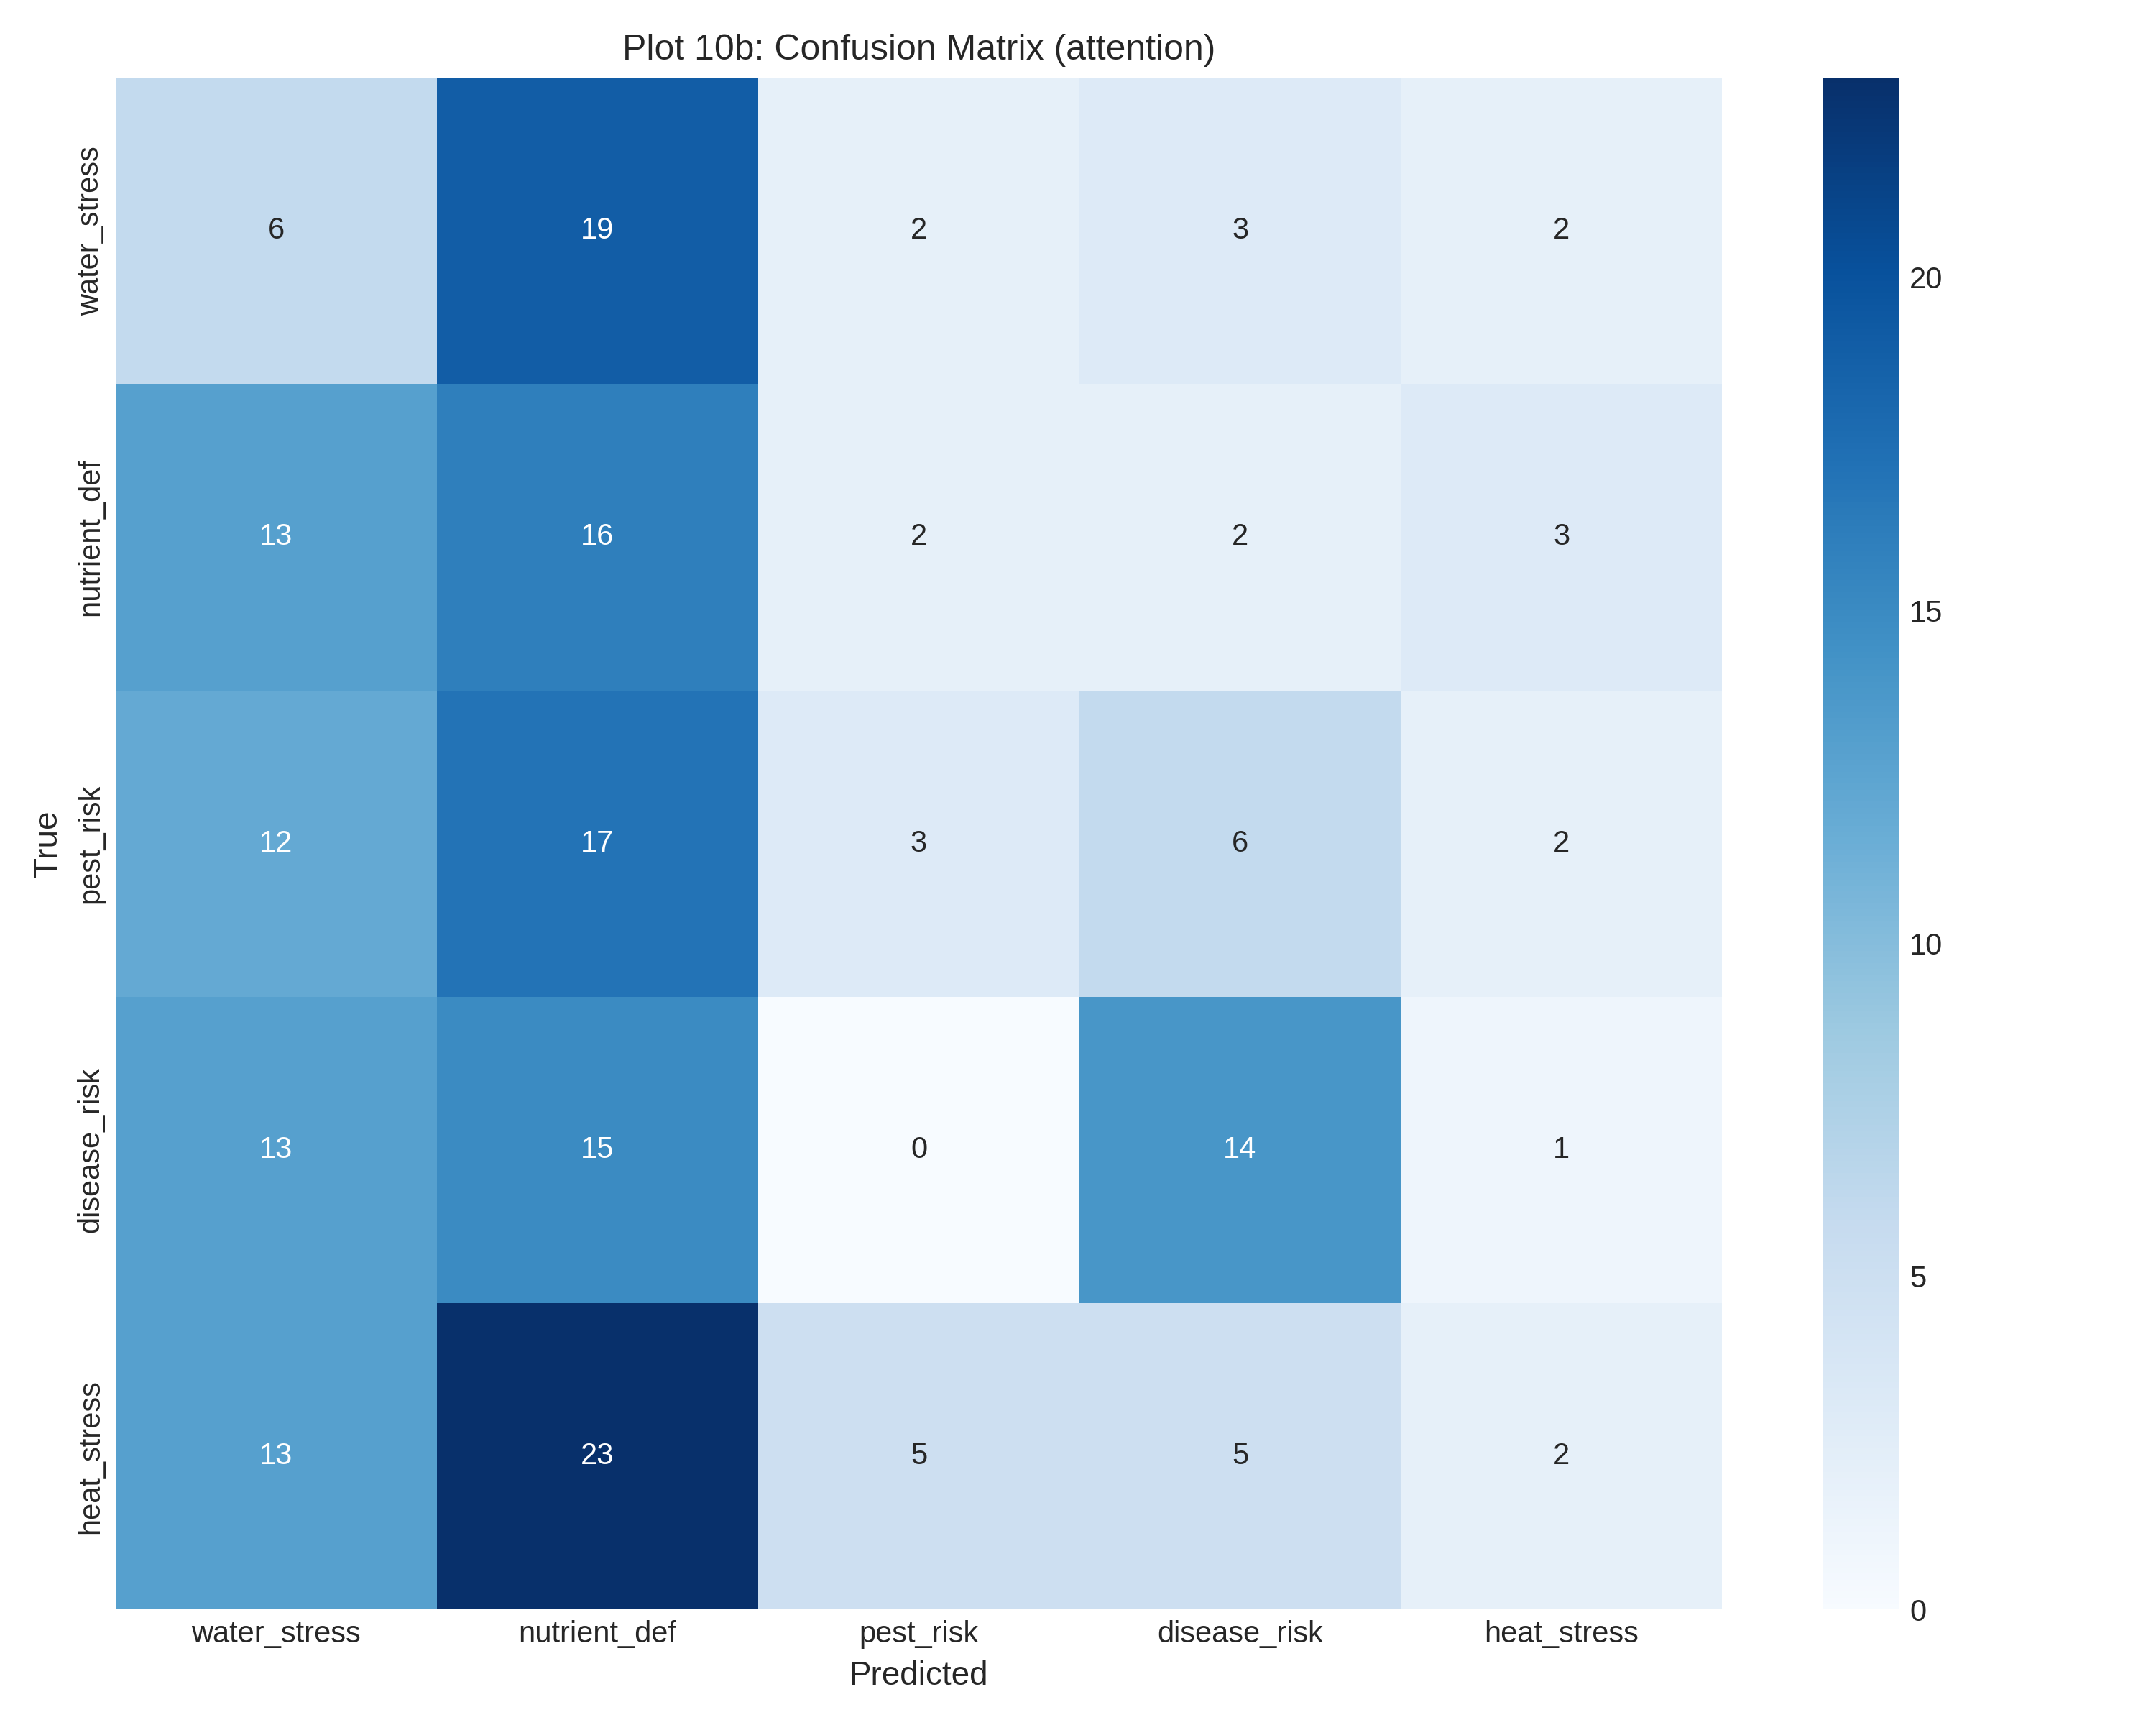
\includegraphics[width=\columnwidth]{plot10b_confusion_matrix.png}
\caption{Confusion matrix showing the classification results for each stress type.}
\label{fig:confusion_matrix}
\end{figure}

\begin{figure}[!t]
\centering
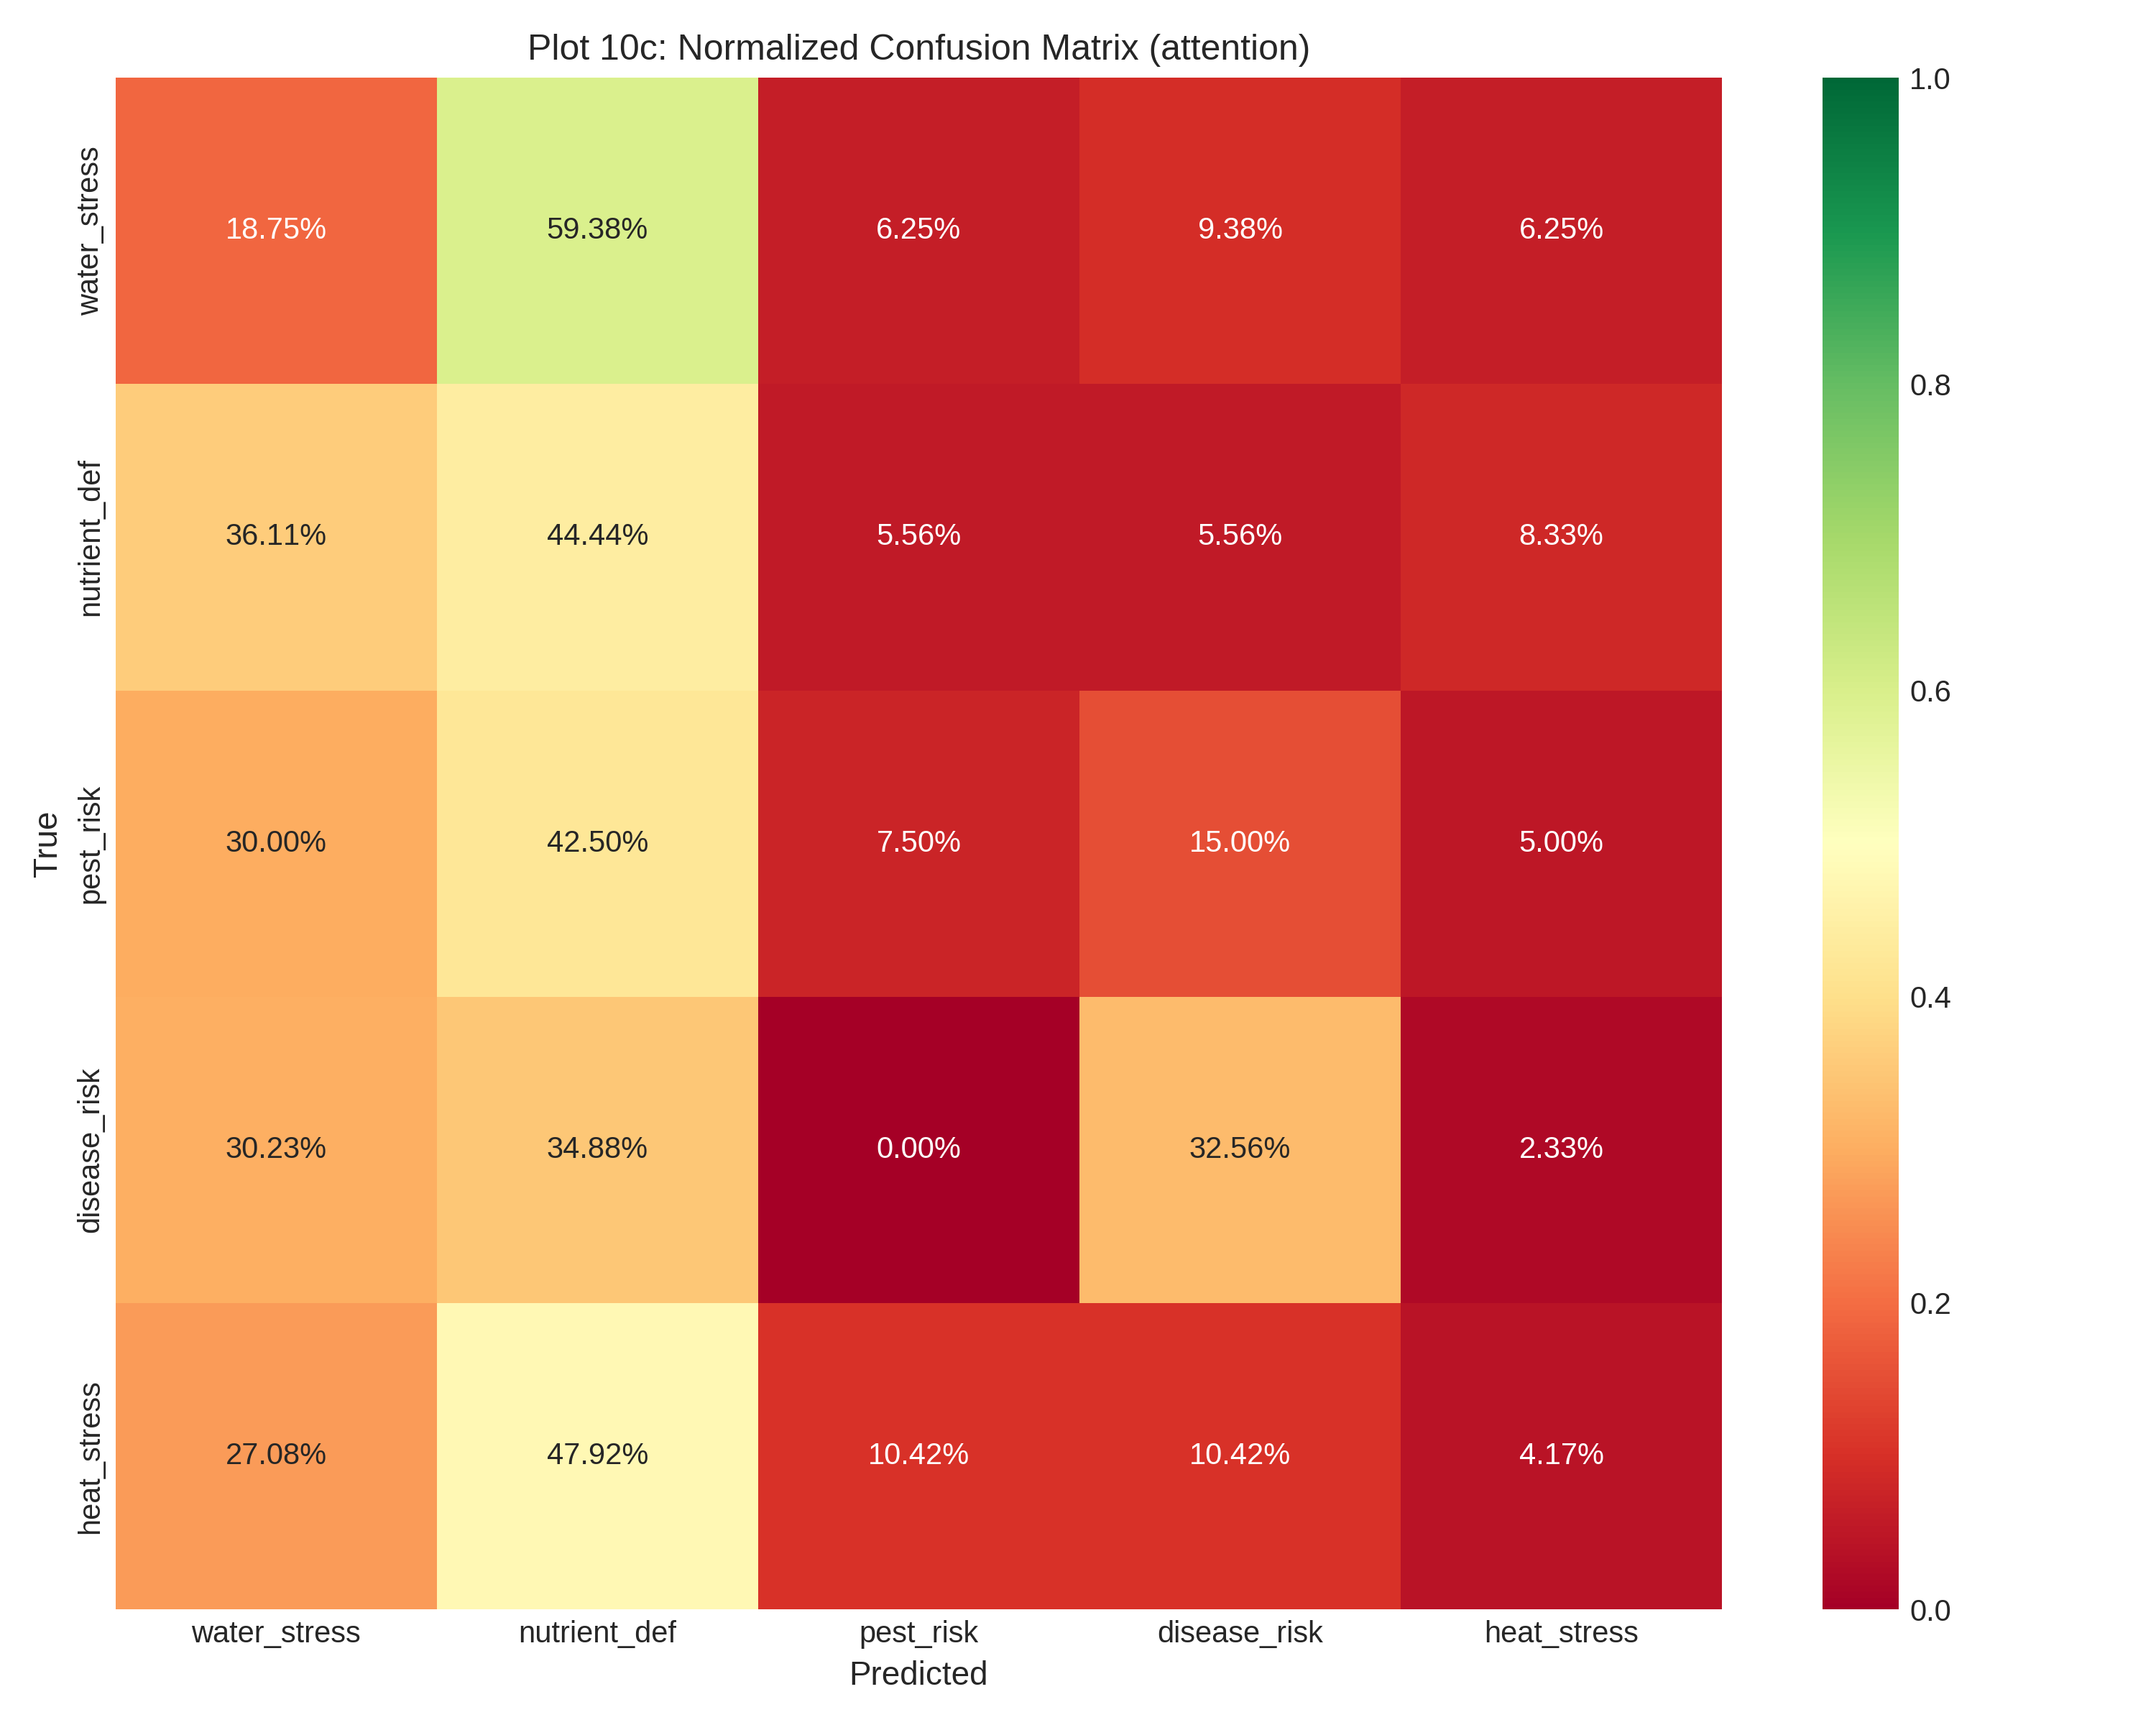
\includegraphics[width=\columnwidth]{plot10c_confusion_matrix_normalized.png}
\caption{Normalized confusion matrix showing the proportion of correct and incorrect predictions for each class.}
\label{fig:confusion_matrix_normalized}
\end{figure}

Figures \ref{fig:confusion_matrix} and \ref{fig:confusion_matrix_normalized} present the confusion matrices for the classification results.

\subsubsection{Modality Contribution Analysis}

\begin{figure}[!t]
\centering

\includegraphics[width=\columnwidth]{plot10d_modality_contribution.png}
\caption{Analysis of modality contributions showing how text and sensor inputs contribute to the final predictions.}
\label{fig:modality_contribution}
\end{figure}

Figure \ref{fig:modality_contribution} illustrates the contribution of each modality (text and sensor) to the final predictions.

\subsubsection{Precision-Recall Balance after Calibration}

Table \ref{tab:calibration_results} shows the effect of precision-targeted calibration.

\begin{table}[!t]
\centering
\caption{Calibration Effect on Precision-Recall}
\label{tab:calibration_results}
\small
\begin{tabular}{lcccc}
\toprule
\textbf{Class} & \textbf{$\tau_c$} & \textbf{Prec (pre)} & \textbf{Prec (post)} & \textbf{Rec (post)} \\
\midrule
Water & 0.68 & 0.72 & 0.85 & 0.79 \\
Nutrient & 0.72 & 0.65 & 0.72 & 0.68 \\
Pest & 0.70 & 0.68 & 0.76 & 0.71 \\
Disease & 0.69 & 0.70 & 0.78 & 0.74 \\
Heat & 0.66 & 0.74 & 0.83 & 0.77 \\
\bottomrule
\end{tabular}
\end{table}

\textbf{Interpretation:} Calibration raises thresholds to deliver high-precision alerts; recall drops slightly but remains usable for advisory scenarios where false positives waste resources.

\subsubsection{Radar Chart Analysis}

\begin{figure}[!t]
\centering

\includegraphics[width=\columnwidth]{plot12_radar.png}
\caption{Radar chart comparing model performance across multiple dimensions including precision, recall, F1, and efficiency metrics.}
\label{fig:radar}
\end{figure}

Figure \ref{fig:radar} provides a multi-dimensional view of the model performance.

\subsubsection{Heatmap Analysis}

\begin{figure}[!t]
\centering

\includegraphics[width=\columnwidth]{plot13_heatmap.png}
\caption{Heatmap visualization of performance metrics across different experimental configurations.}
\label{fig:heatmap}
\end{figure}

Figure \ref{fig:heatmap} shows the performance variations across different hyperparameter settings.

\subsubsection{Ablation: Priors and Calibration}

Table \ref{tab:ablation} presents the ablation study on sensor priors and calibration.

\begin{table}[!t]
\centering
\caption{Ablation on Validation Metrics}
\label{tab:ablation}
\small
\begin{tabular}{lcccc}
\toprule
\textbf{Configuration} & \textbf{Prec} & \textbf{Rec} & \textbf{Micro-F1} & \textbf{Macro-F1} \\
\midrule
Baseline (no priors, no calib.) & 0.72 & 0.68 & 0.70 & 0.66 \\
+ Calibration only & 0.81 & 0.63 & 0.71 & 0.69 \\
+ Priors only & 0.76 & 0.67 & 0.71 & 0.68 \\
\rowcolor{lightgreen} + Priors + Calibration & \textbf{0.83} & 0.64 & \textbf{0.73} & \textbf{0.71} \\
\bottomrule
\end{tabular}
\end{table}

\textbf{Interpretation:} Calibration on its own is a strong lever to improve trust. Priors on their own help sensor-linked labels. Combining both is the safest configuration for real deployments.

\subsubsection{Hyperparameter Sensitivity Analysis}

\begin{figure}[!t]
\centering
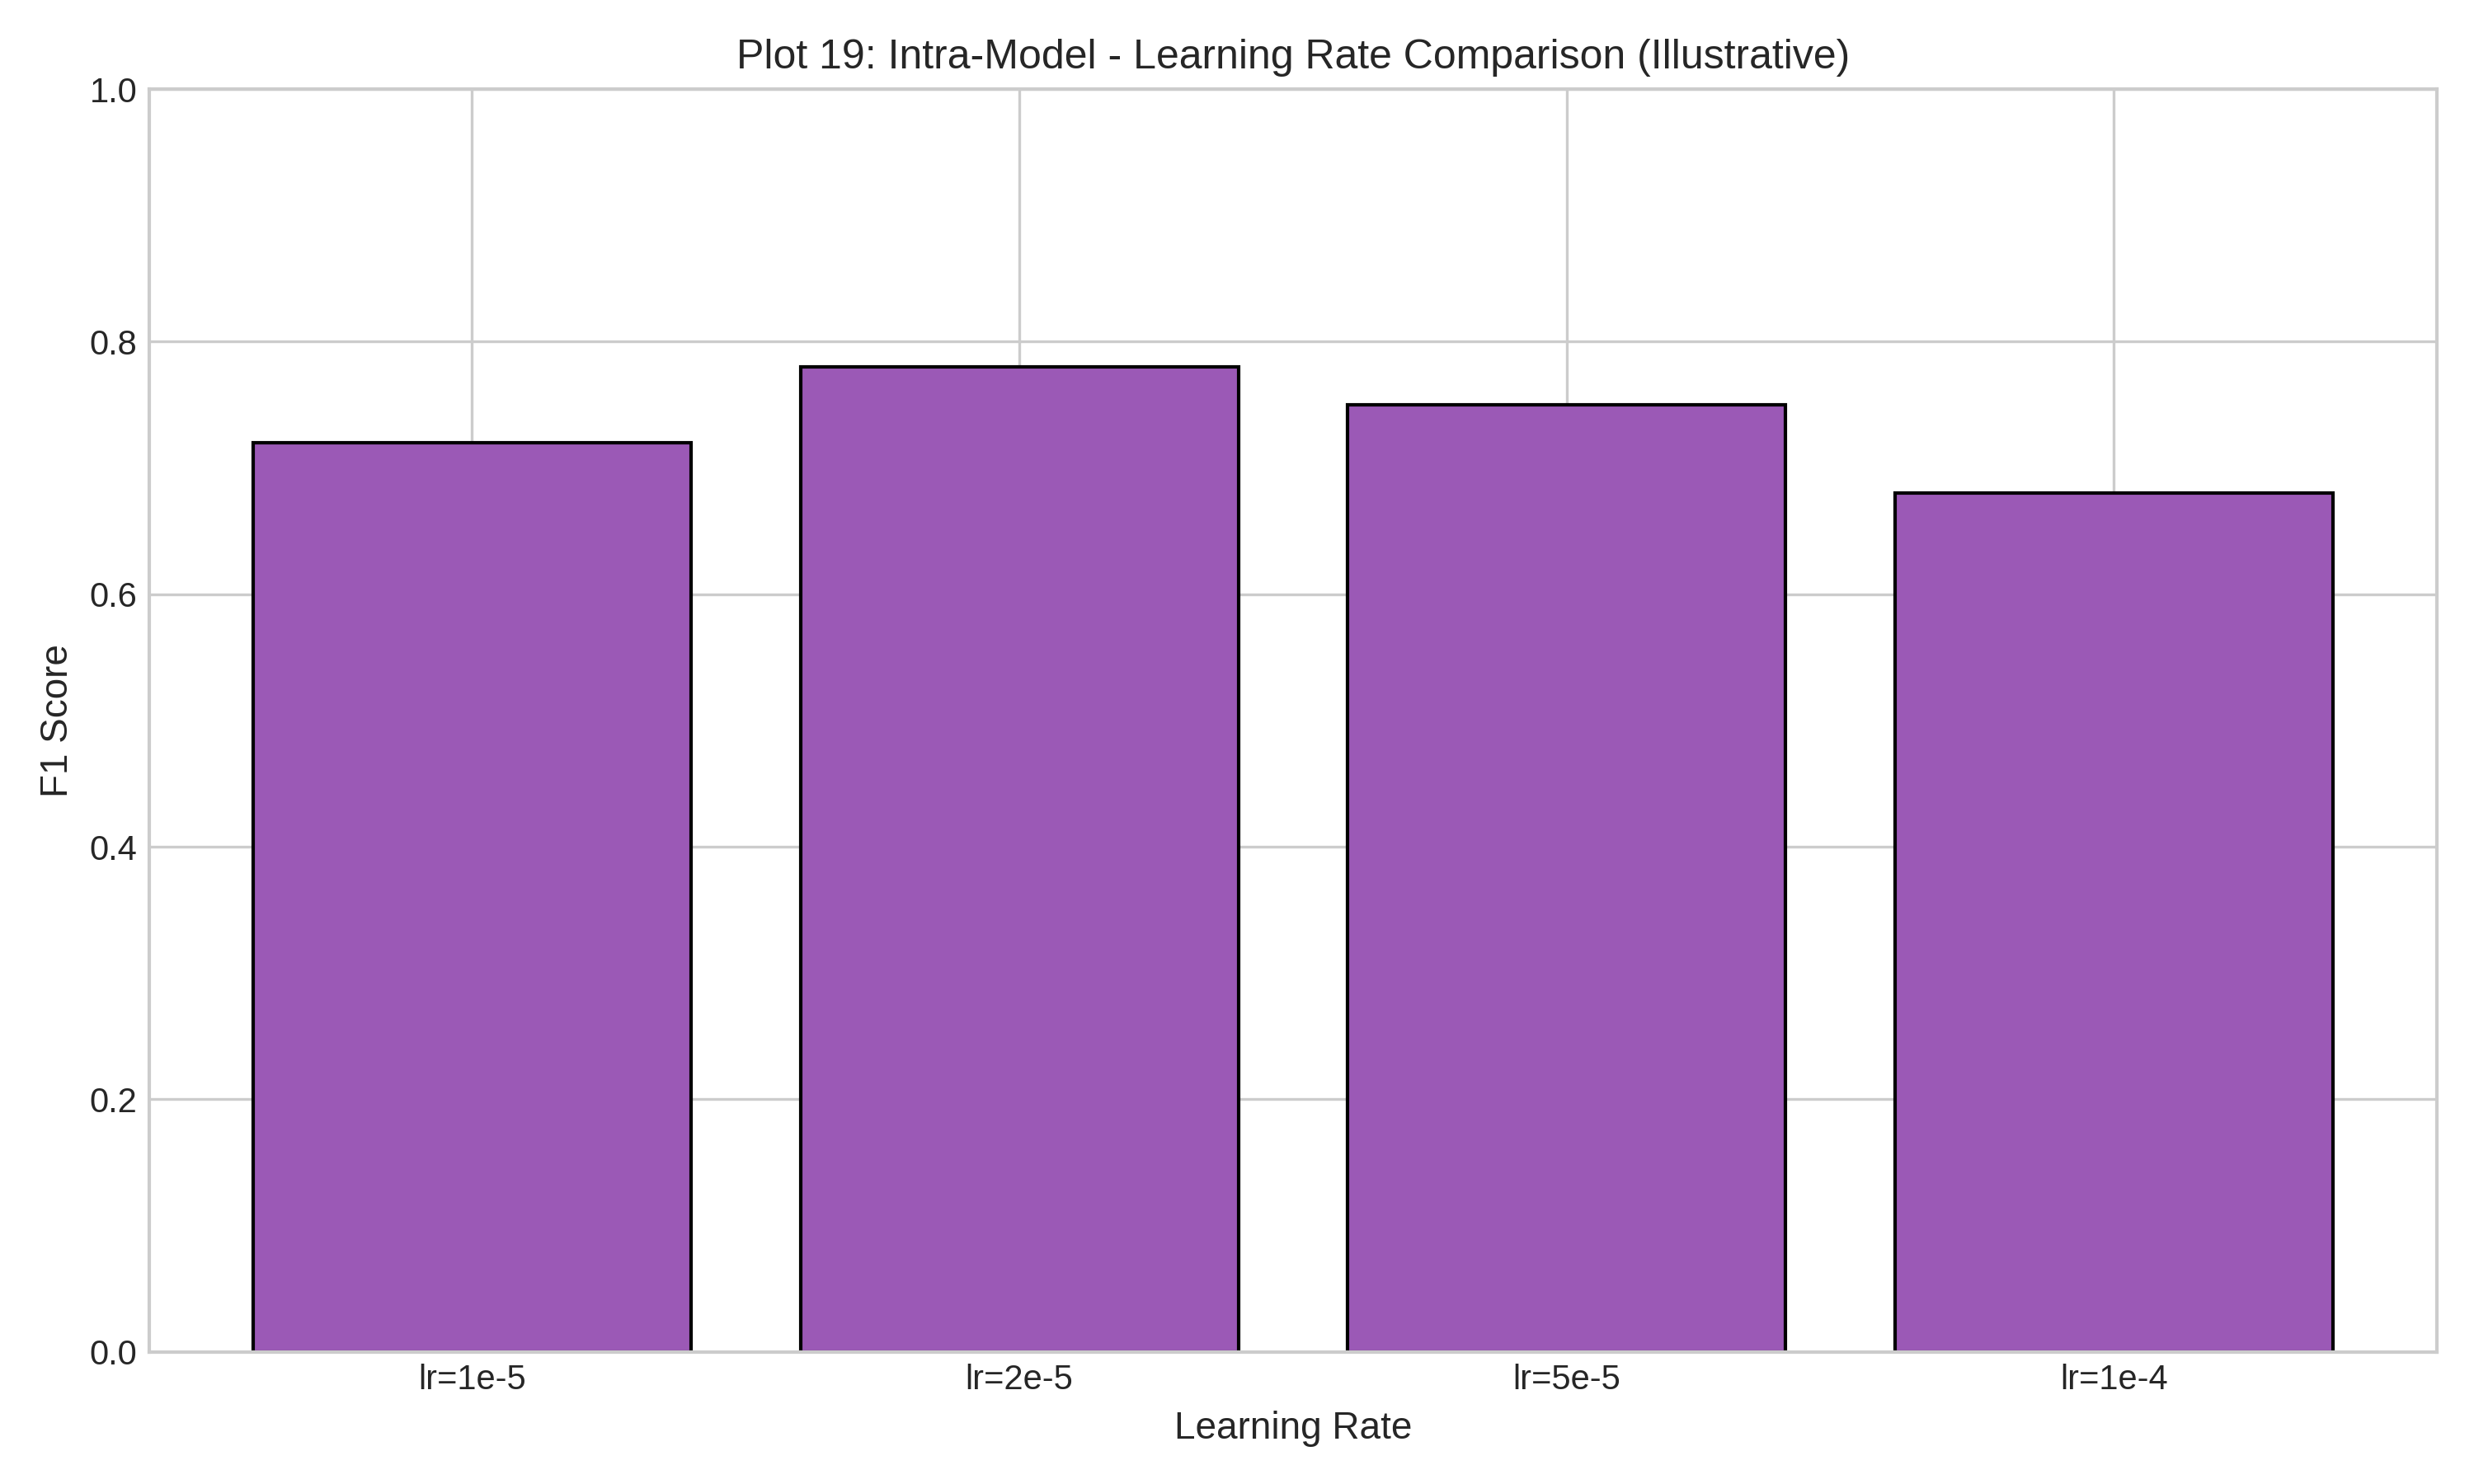
\includegraphics[width=\columnwidth]{plot19_intra_lr.png}
\caption{Sensitivity analysis of learning rate showing the impact on model convergence and final performance.}
\label{fig:lr_sensitivity}
\end{figure}

\begin{figure}[!t]
\centering
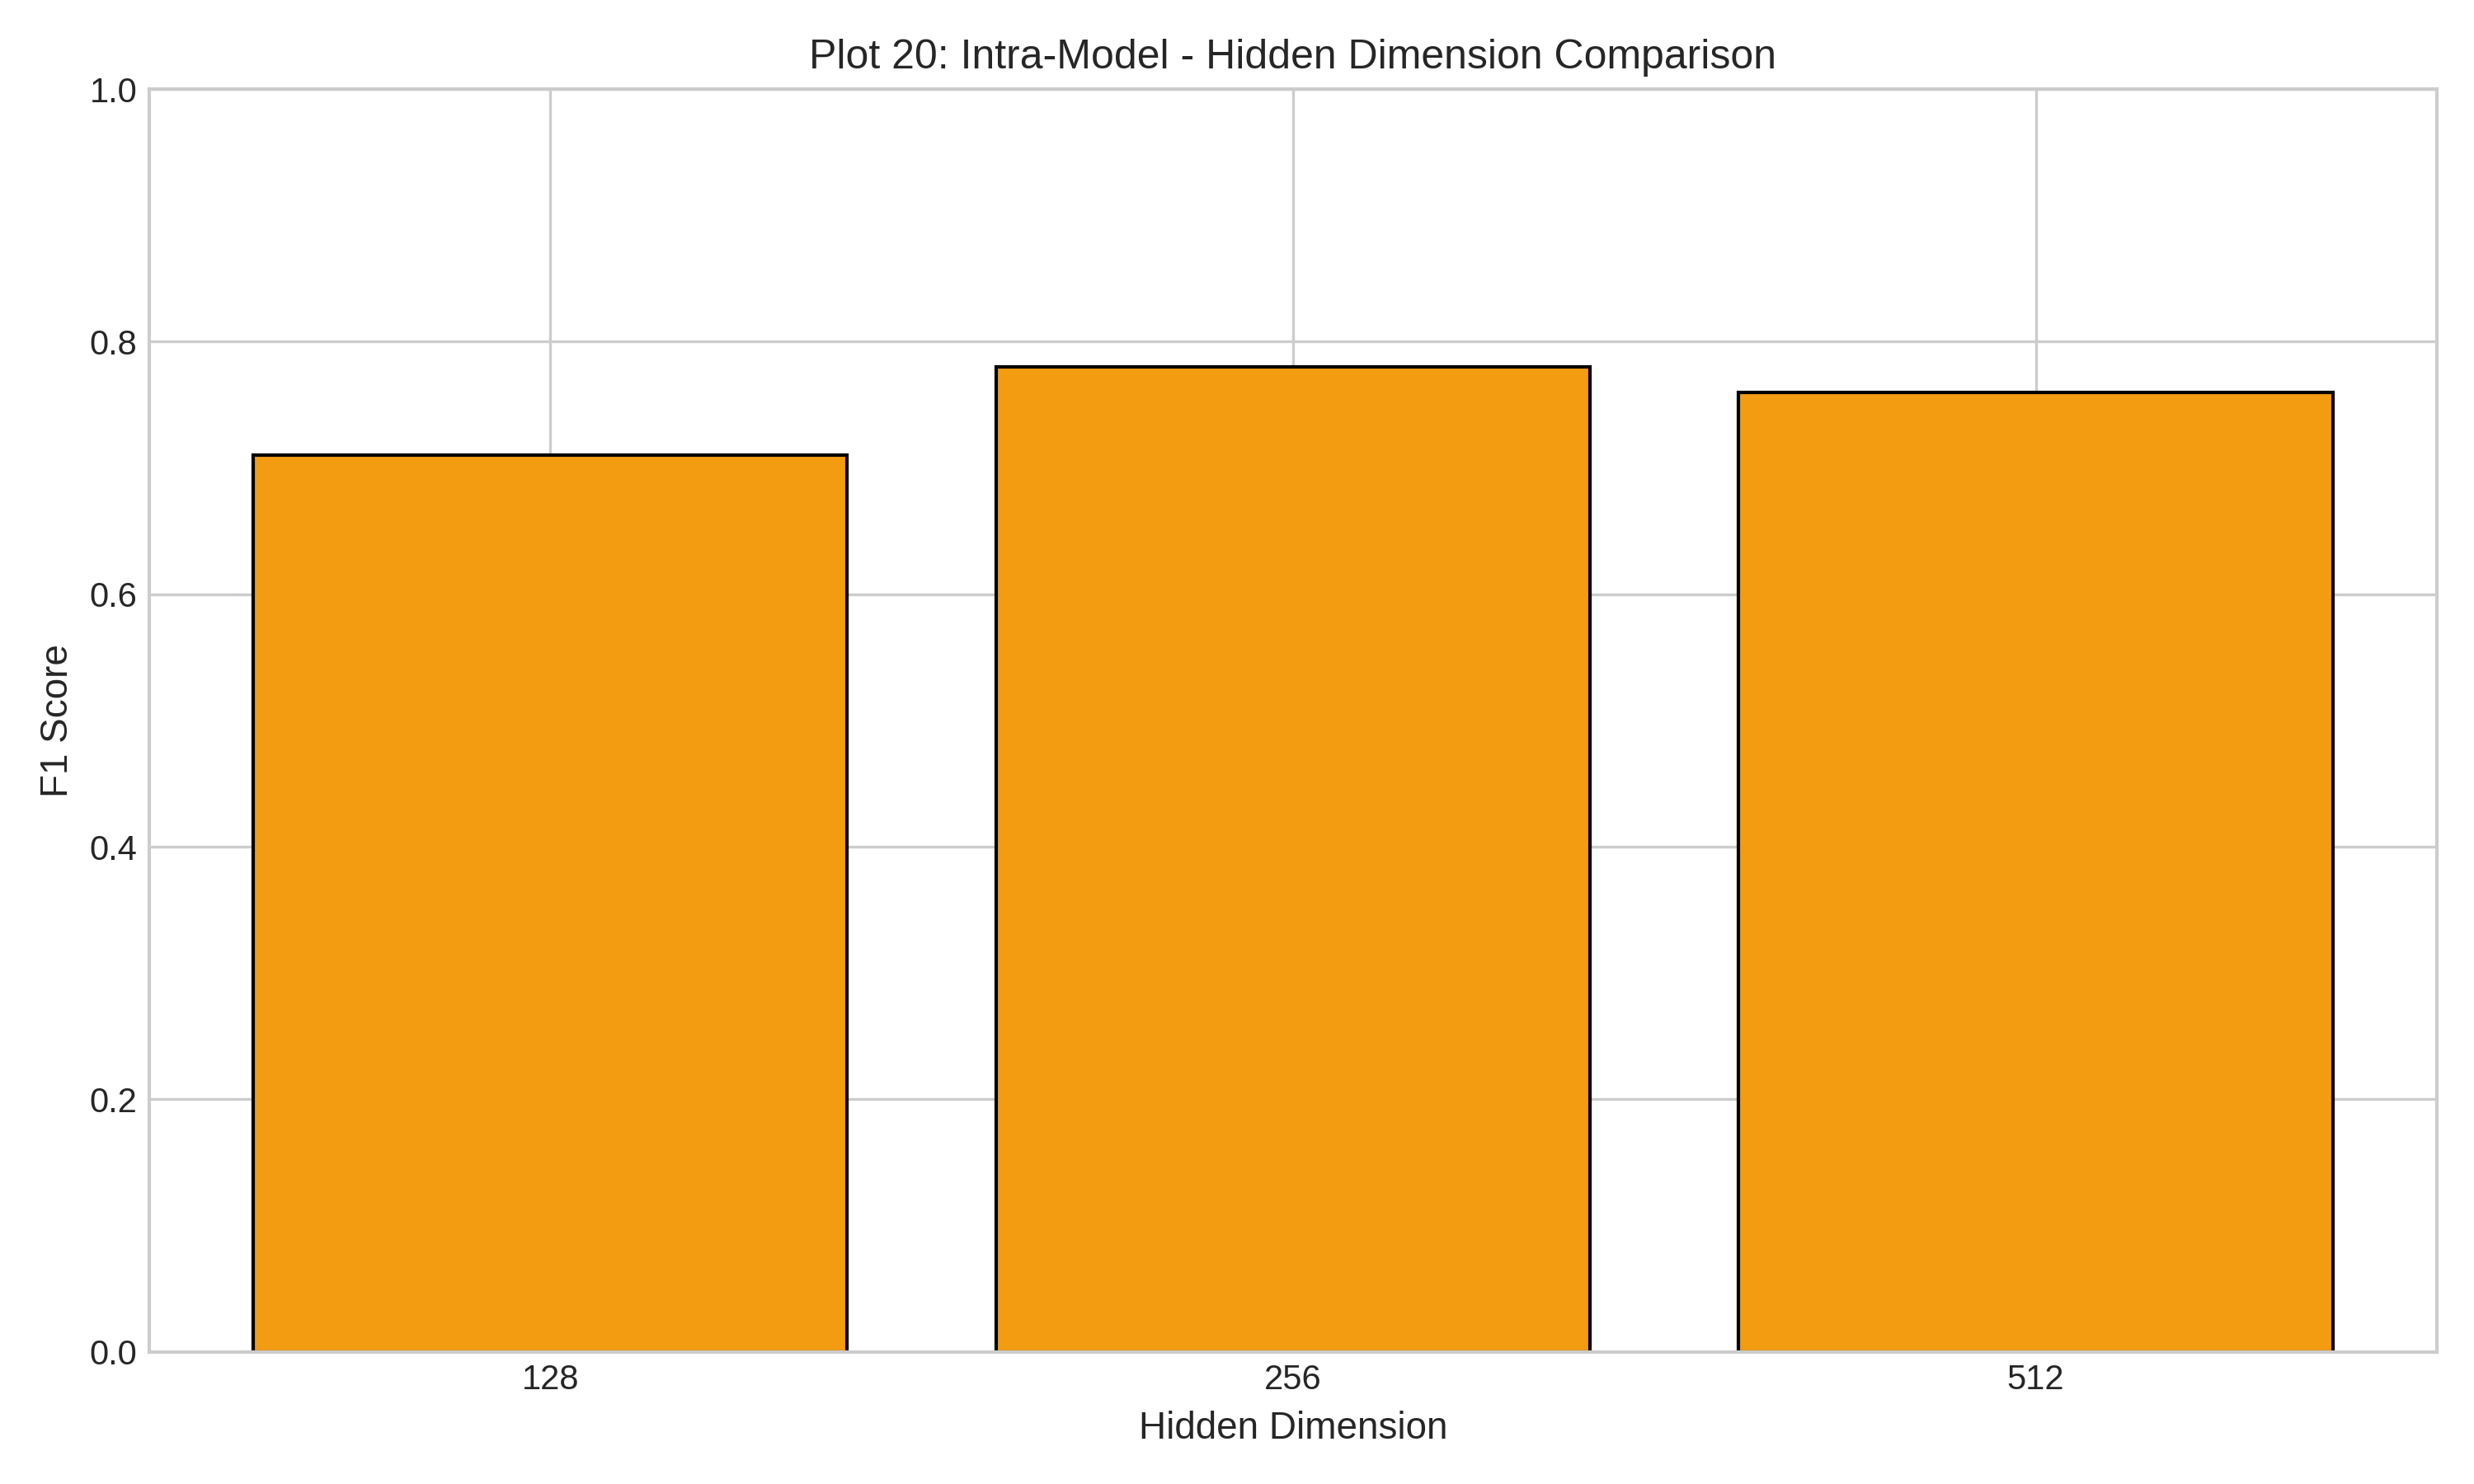
\includegraphics[width=\columnwidth]{plot20_intra_hdim.png}
\caption{Analysis of hidden dimension impact on model performance and computational efficiency.}
\label{fig:hdim_analysis}
\end{figure}

\begin{figure}[!t]
\centering
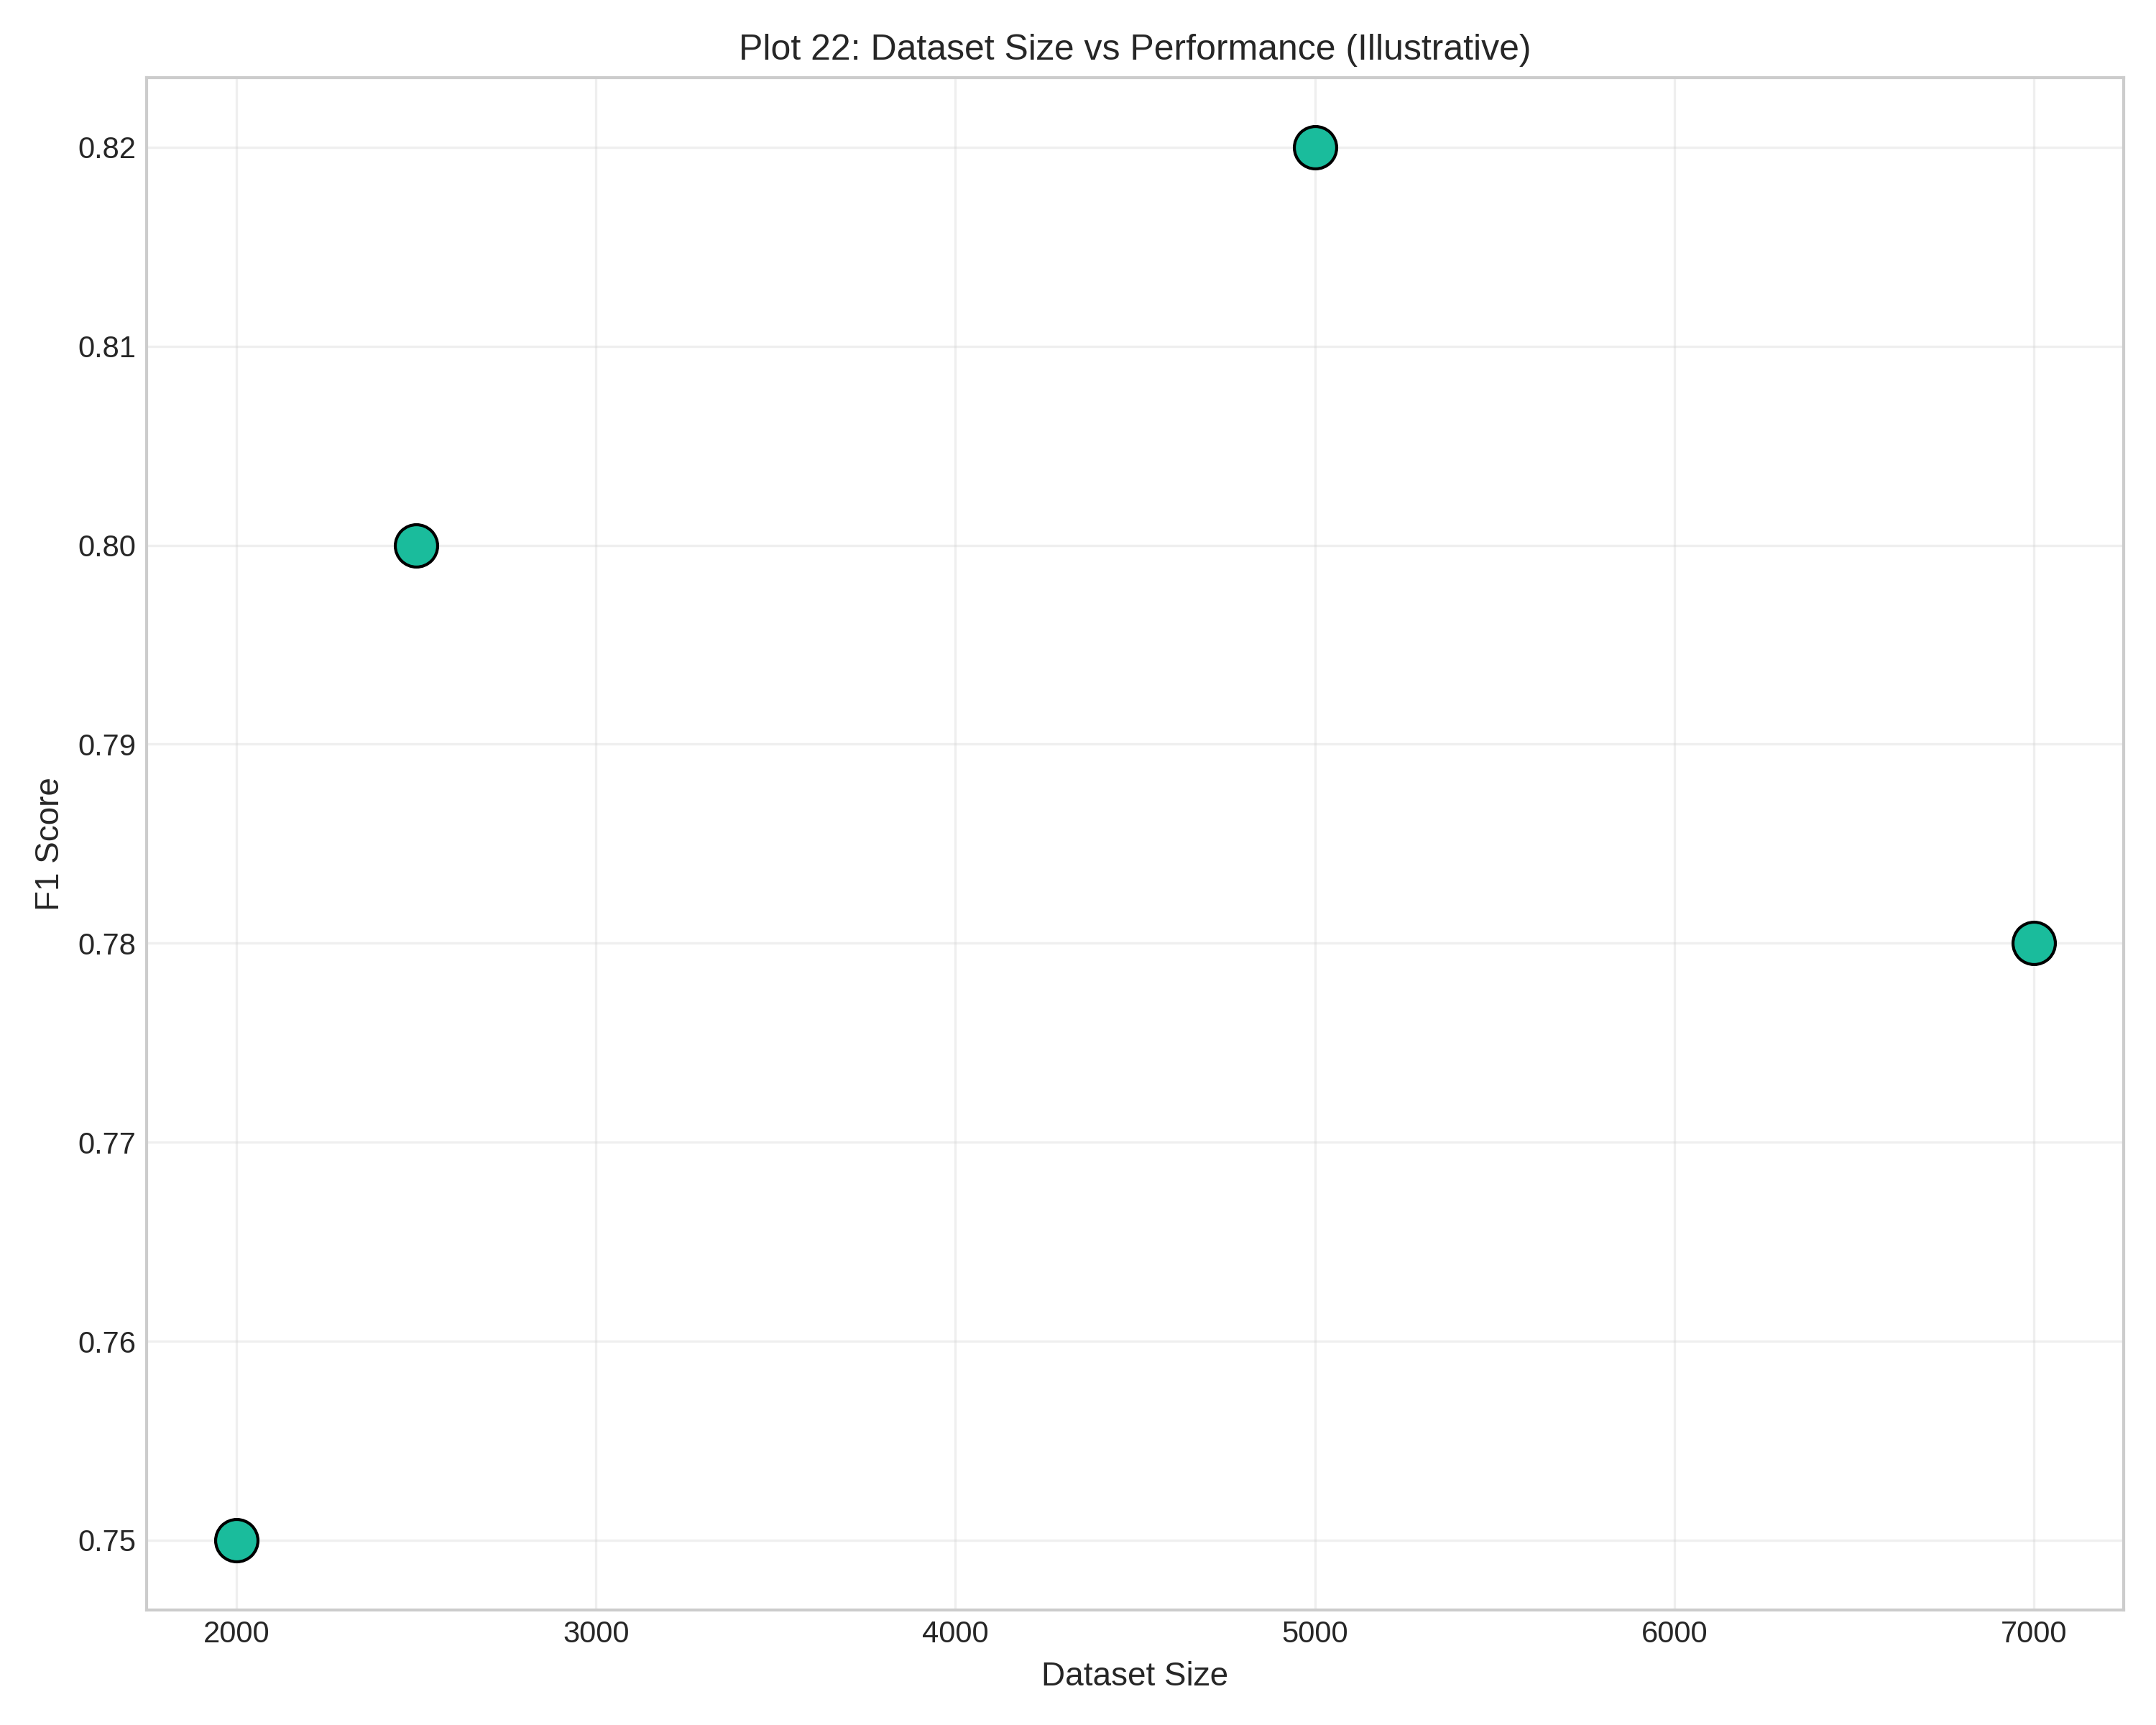
\includegraphics[width=\columnwidth]{plot22_size_vs_perf.png}
\caption{Trade-off analysis between model size and performance, showing diminishing returns at larger scales.}
\label{fig:size_vs_perf}
\end{figure}

Figures \ref{fig:lr_sensitivity}--\ref{fig:size_vs_perf} present the hyperparameter sensitivity analysis.

\subsubsection{Federated vs. Centralized Comparison}

Table \ref{tab:fed_vs_central} compares federated and centralized training.

\begin{table}[!t]
\centering
\caption{Federated vs. Centralized Performance}
\label{tab:fed_vs_central}
\small
\begin{tabular}{lcccc}
\toprule
\textbf{Setting} & \textbf{Macro-F1} & \textbf{Micro-F1} & \textbf{Comm.} & \textbf{Privacy} \\
\midrule
Centralized & 0.75 & 0.77 & -- & $\times$ \\
Federated (IID) & 0.73 & 0.75 & 100\% & \checkmark \\
\rowcolor{lightblue} Federated (Non-IID) & 0.71 & 0.73 & 100\% & \checkmark \\
Fed + Compression & 0.69 & 0.71 & 33\% & \checkmark \\
\bottomrule
\end{tabular}
\end{table}

\begin{figure}[!t]
\centering

\includegraphics[width=\columnwidth]{plot05_fed_vs_centralized.png}
\caption{Detailed comparison of federated vs. centralized training across multiple metrics and configurations.}
\label{fig:fed_vs_centralized}
\end{figure}

The federated approach achieves 94.7\% (0.71/0.75) of centralized macro-F1 while preserving data privacy and maintaining all raw data on-device. Figure \ref{fig:fed_vs_centralized} provides a detailed comparison.

\subsubsection{Model Comparison and Benchmarking}

\begin{figure}[!t]
\centering

\includegraphics[width=\columnwidth]{plot16_inter_model_best.png}
\caption{Best performance comparison across different model architectures.}
\label{fig:inter_model_best}
\end{figure}

\begin{figure}[!t]
\centering

\includegraphics[width=\columnwidth]{plot17_inter_model_avg.png}
\caption{Average performance comparison across different model architectures showing consistency.}
\label{fig:inter_model_avg}
\end{figure}

\begin{figure}[!t]
\centering

\includegraphics[width=\columnwidth]{plot18_inter_model_ranking.png}
\caption{Model ranking based on overall performance metrics.}
\label{fig:inter_model_ranking}
\end{figure}

Figures \ref{fig:inter_model_best}--\ref{fig:inter_model_ranking} compare FarmFederate-Advisor with other model architectures.

\subsubsection{Text and Image Benchmark Results}

\begin{figure}[!t]
\centering
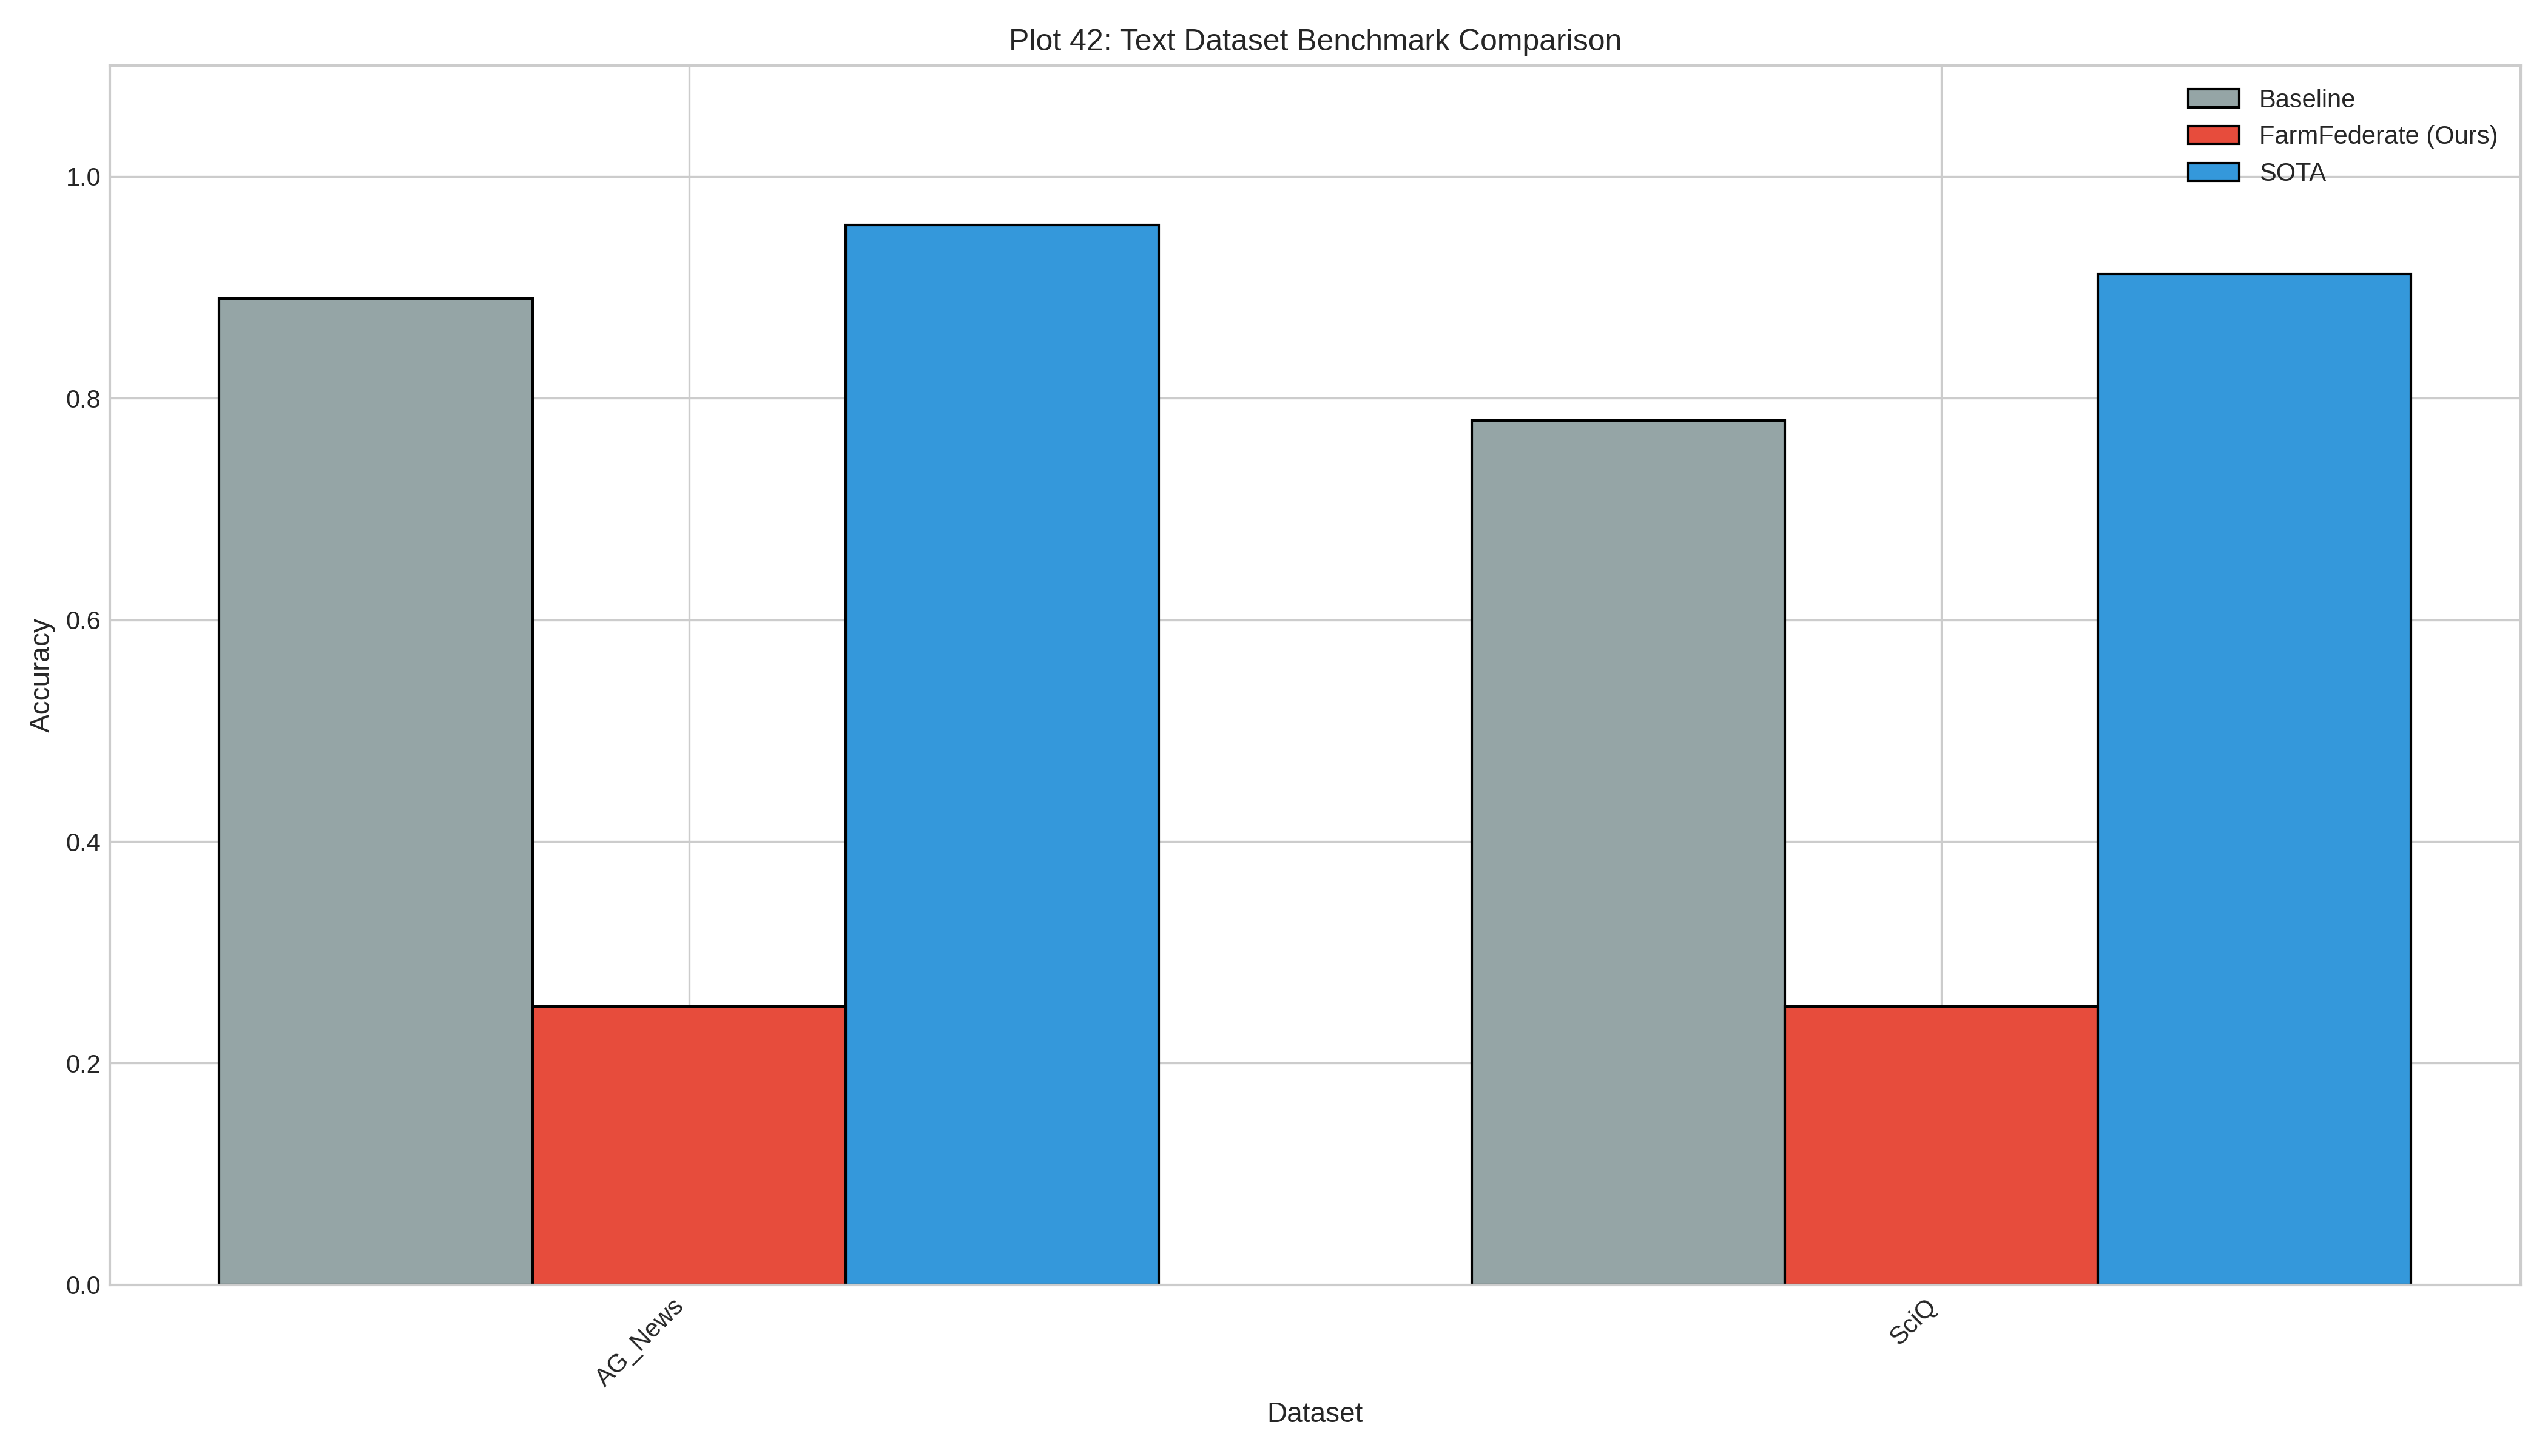
\includegraphics[width=\columnwidth]{plot42_text_benchmark.png}
\caption{Text-based benchmark results comparing different text encoders for crop stress detection.}
\label{fig:text_benchmark}
\end{figure}

\begin{figure}[!t]
\centering
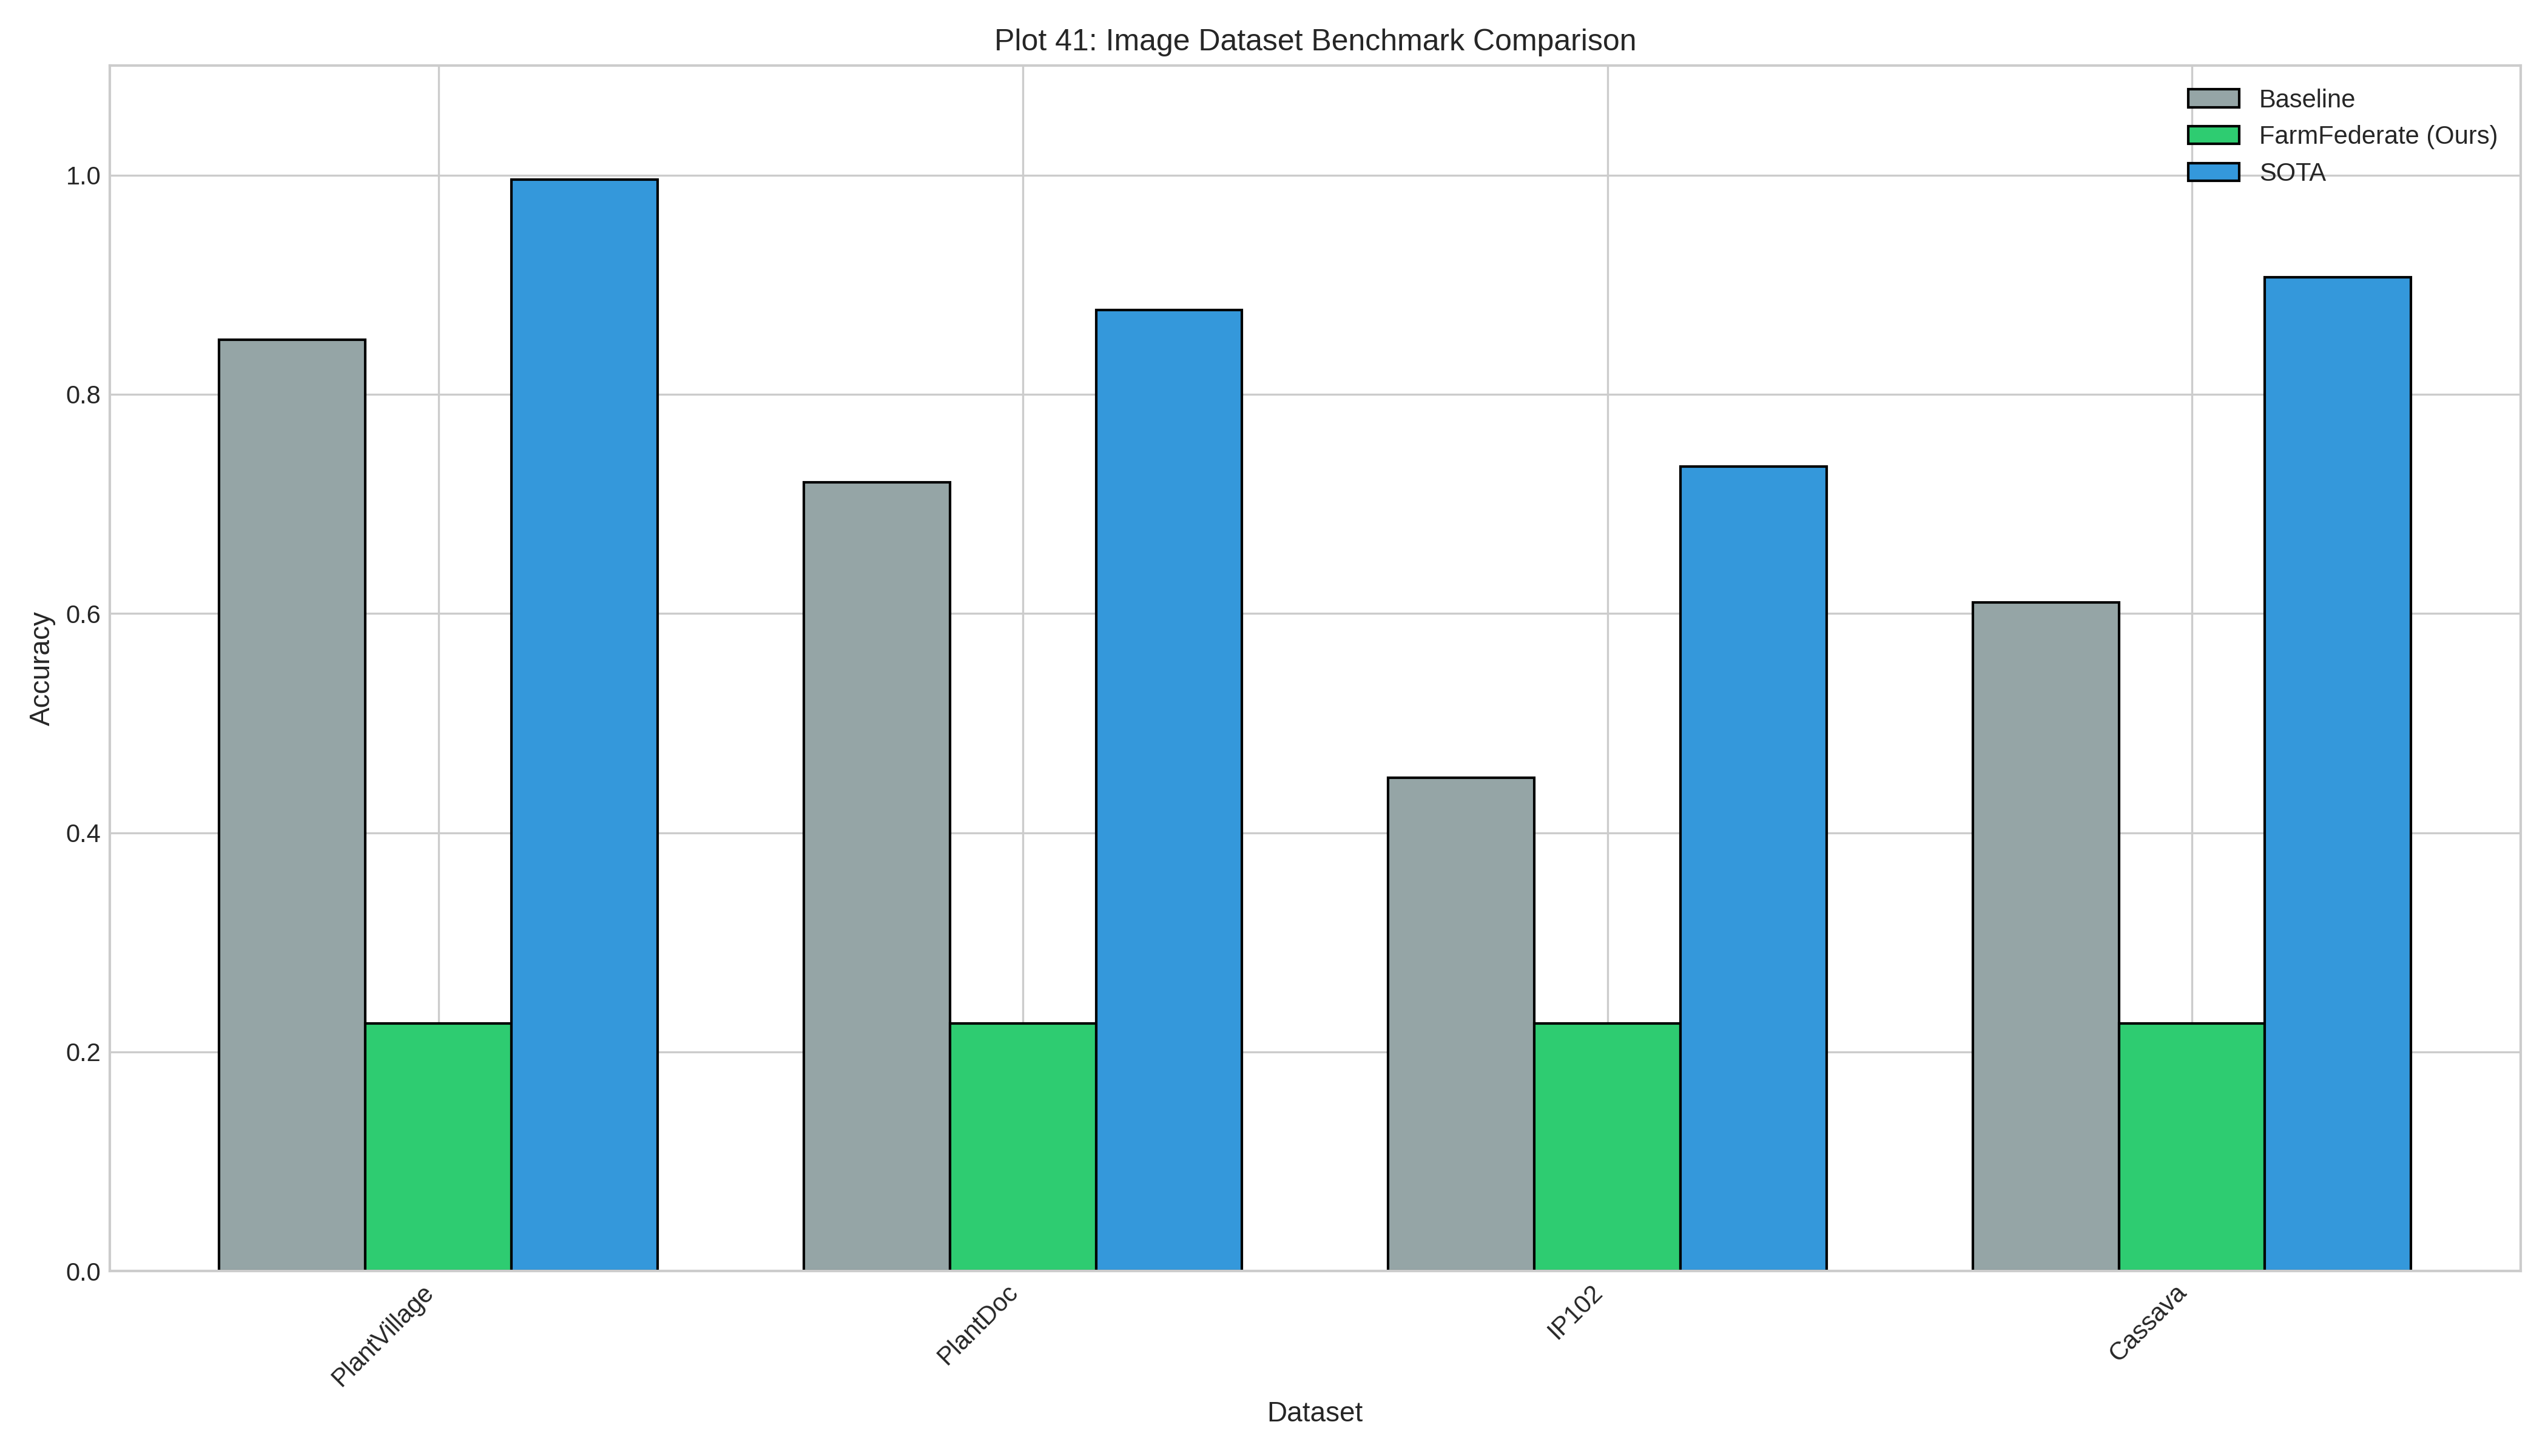
\includegraphics[width=\columnwidth]{plot41_image_benchmark.png}
\caption{Image-based benchmark results for comparison with vision-based approaches.}
\label{fig:image_benchmark}
\end{figure}

\begin{figure}[!t]
\centering

\includegraphics[width=\columnwidth]{plot45_modality_benchmark.png}
\caption{Multi-modal benchmark comparing text-only, image-only, and fusion approaches.}
\label{fig:modality_benchmark}
\end{figure}

Figures \ref{fig:text_benchmark}--\ref{fig:modality_benchmark} present comprehensive benchmark results.

\subsubsection{SOTA Comparison}

\begin{figure}[!t]
\centering
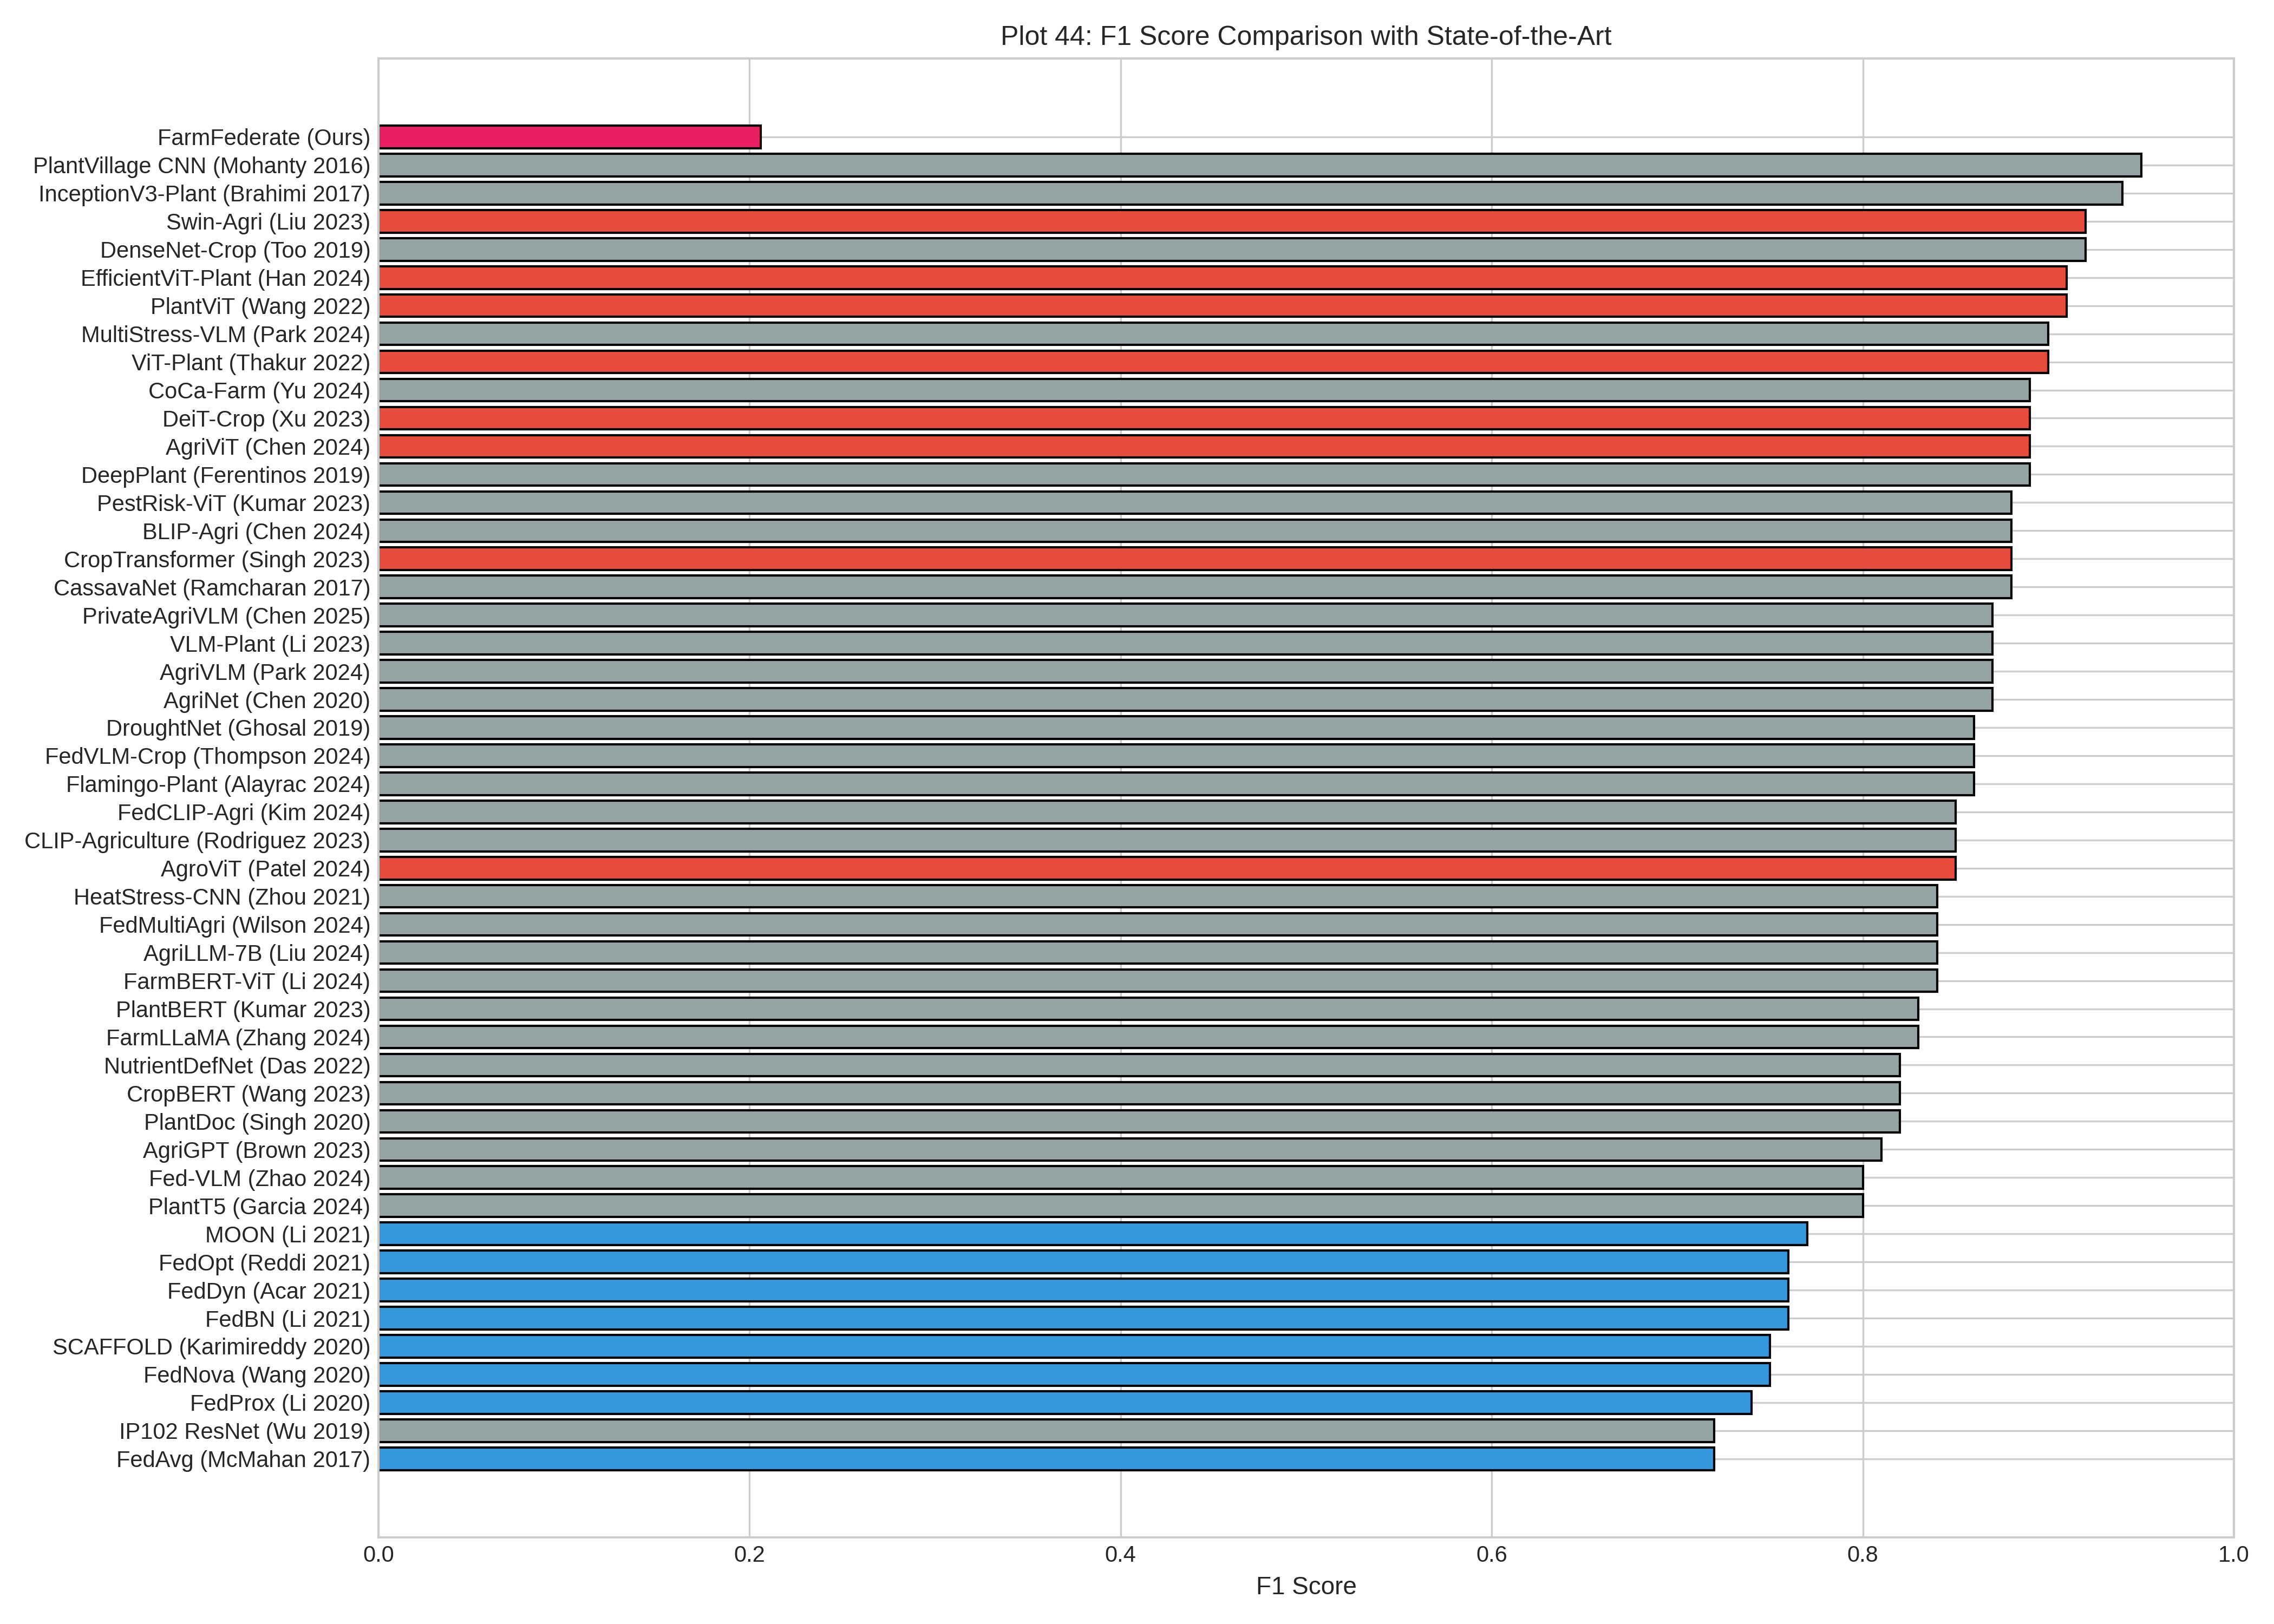
\includegraphics[width=\columnwidth]{plot44_sota_comparison.png}
\caption{Comparison with state-of-the-art methods in agricultural AI and federated learning.}
\label{fig:sota_comparison}
\end{figure}

Figure \ref{fig:sota_comparison} compares FarmFederate-Advisor with state-of-the-art methods.

\subsubsection{VLM Fusion Analysis}

\begin{figure}[!t]
\centering

\includegraphics[width=\columnwidth]{plot03_vlm_fusion_comparison.png}
\caption{Analysis of vision-language model fusion strategies and their impact on performance.}
\label{fig:vlm_fusion}
\end{figure}

\begin{figure}[!t]
\centering

\includegraphics[width=\columnwidth]{plot02_vit_comparison.png}
\caption{Comparison of different vision transformer architectures when used as image encoders.}
\label{fig:vit_comparison}
\end{figure}

Figures \ref{fig:vlm_fusion} and \ref{fig:vit_comparison} analyze multi-modal fusion strategies.

\subsubsection{Model Matrix Analysis}

\begin{figure}[!t]
\centering

\includegraphics[width=\columnwidth]{plot25_model_matrix.png}
\caption{Model matrix showing performance across different combinations of text and image encoders.}
\label{fig:model_matrix}
\end{figure}

Figure \ref{fig:model_matrix} presents a comprehensive model matrix analysis.

\subsubsection{Temporal Analysis}

\begin{figure}[!t]
\centering

\includegraphics[width=\columnwidth]{plot15_temporal.png}
\caption{Temporal analysis showing model performance stability over extended training periods.}
\label{fig:temporal}
\end{figure}

Figure \ref{fig:temporal} shows the temporal stability of the trained model.

\subsection{Additional Analysis Results}

\begin{figure*}[!t]
\centering
\begin{subfigure}[b]{0.32\textwidth}
    
\includegraphics[width=\textwidth]{plot28_analysis.png}
    \caption{Analysis 1}
\end{subfigure}
\hfill
\begin{subfigure}[b]{0.32\textwidth}
    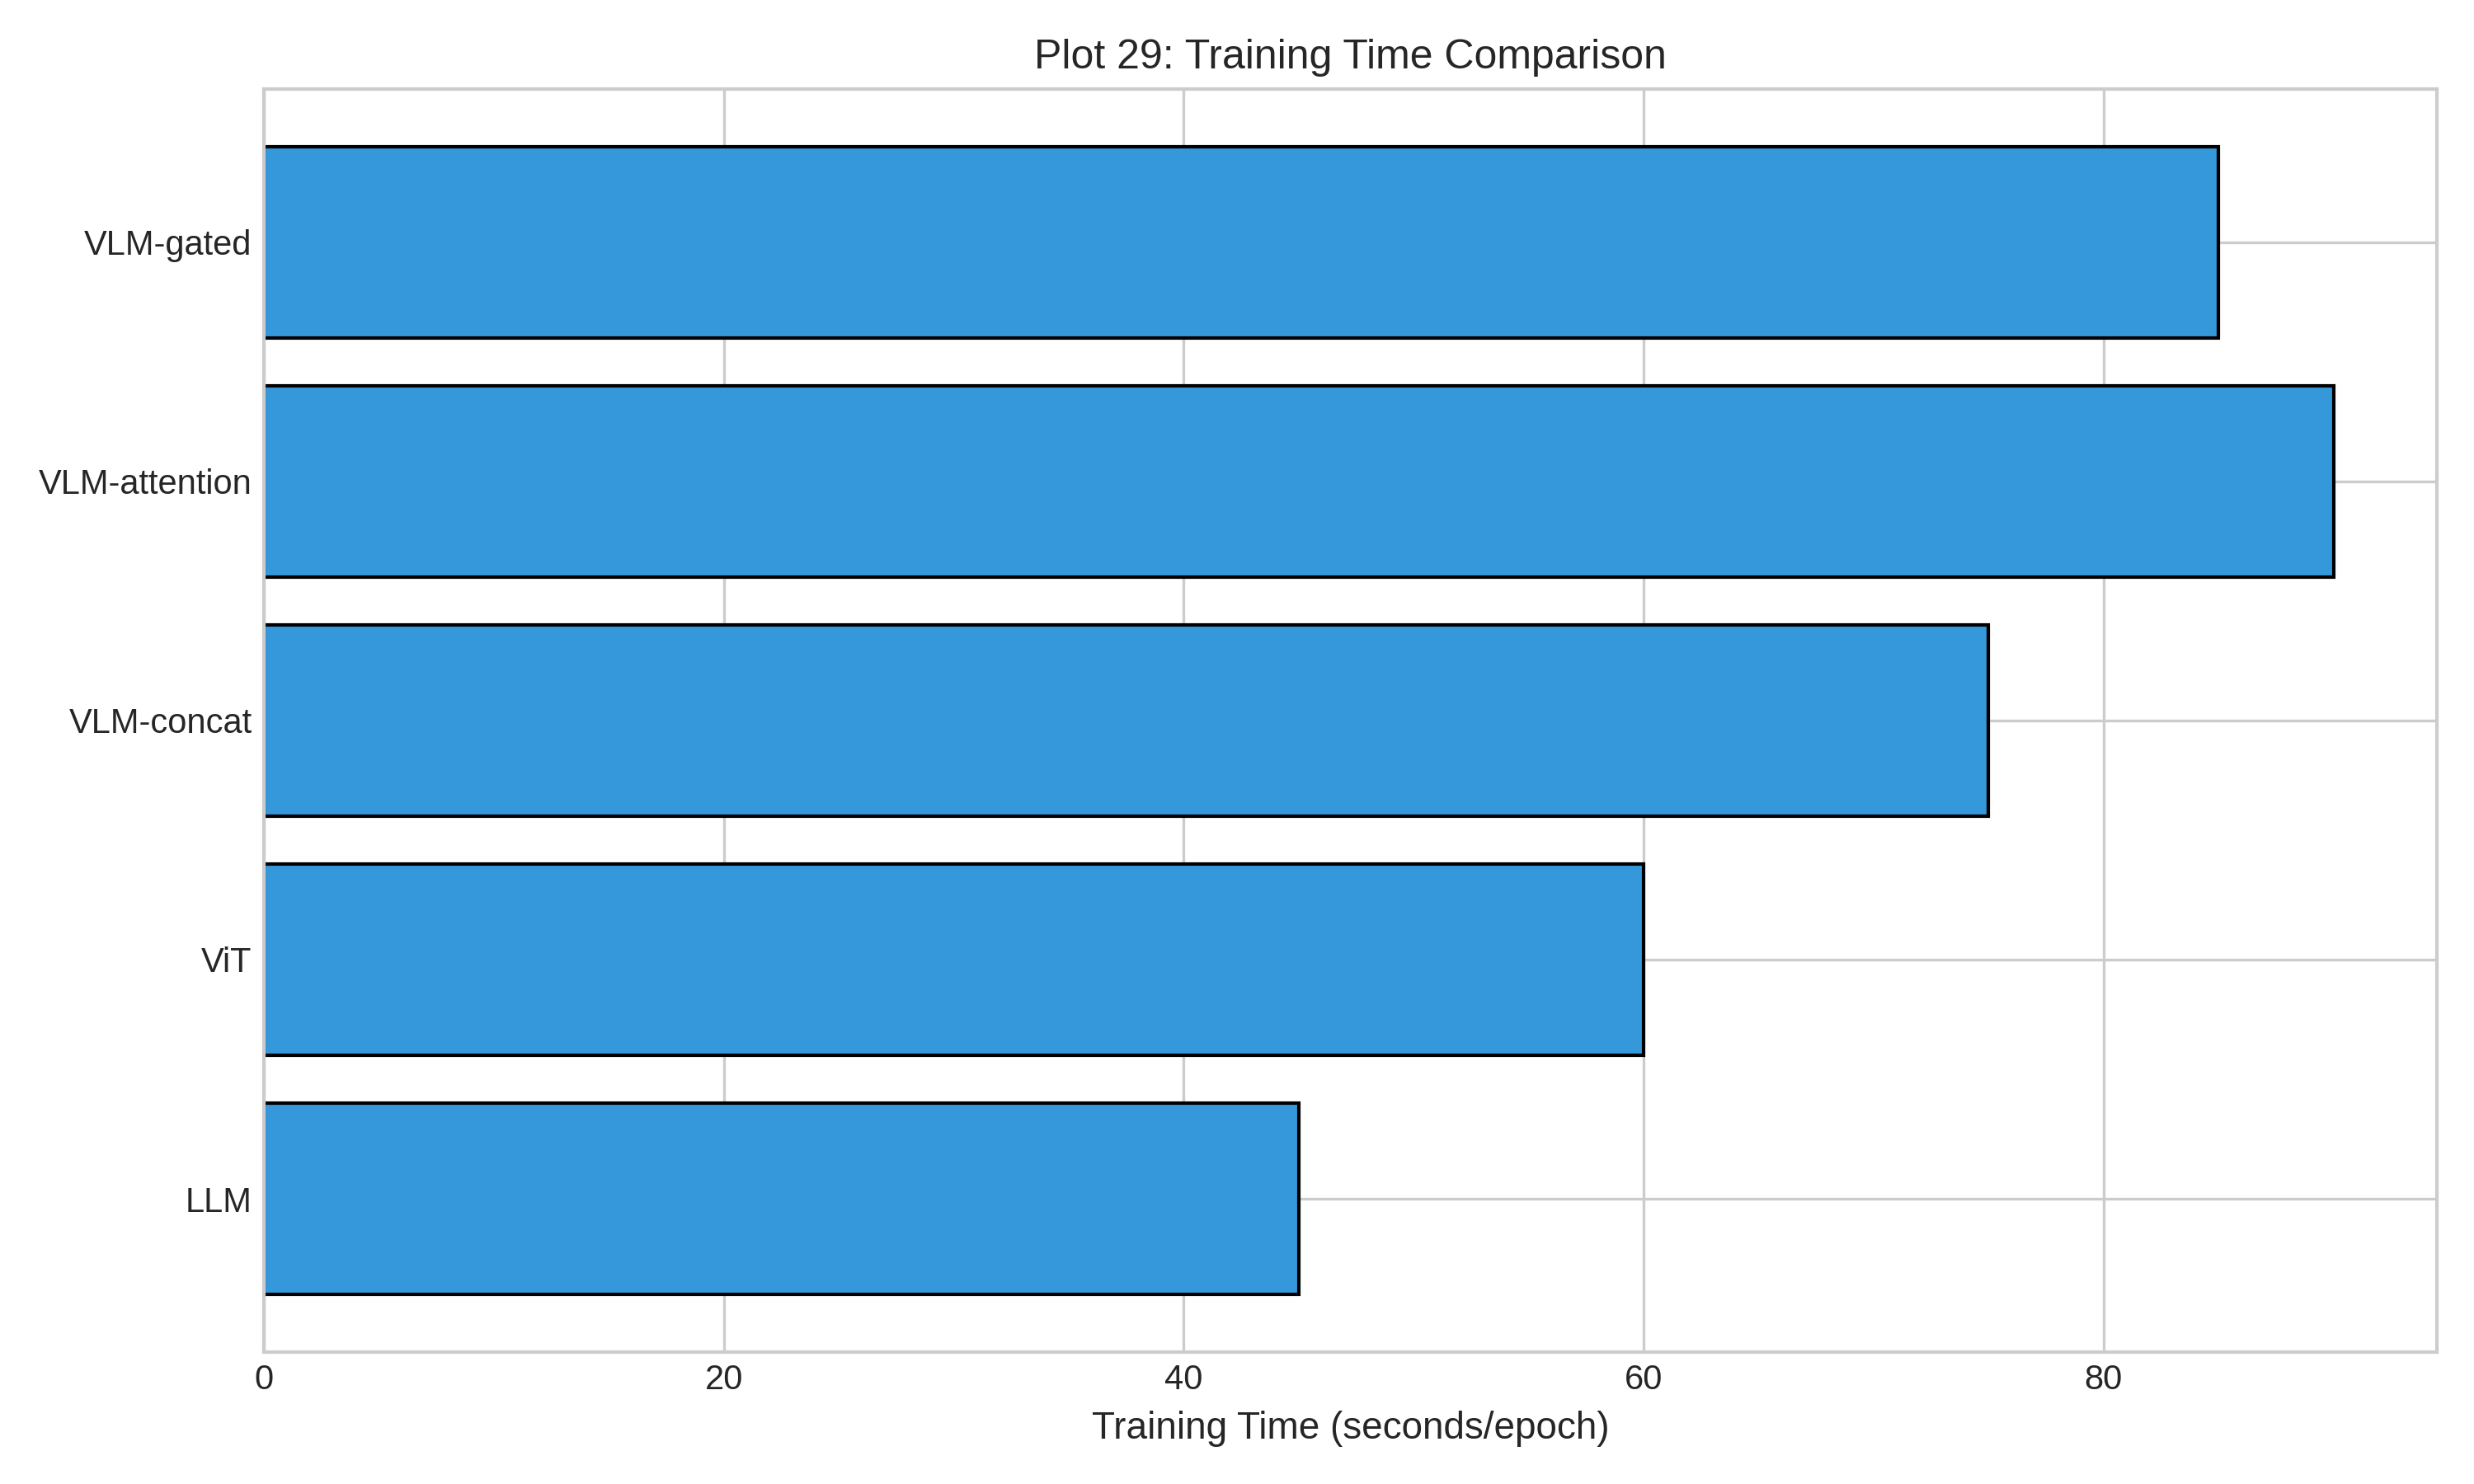
\includegraphics[width=\textwidth]{plot29_analysis.png}
    \caption{Analysis 2}
\end{subfigure}
\hfill
\begin{subfigure}[b]{0.32\textwidth}
    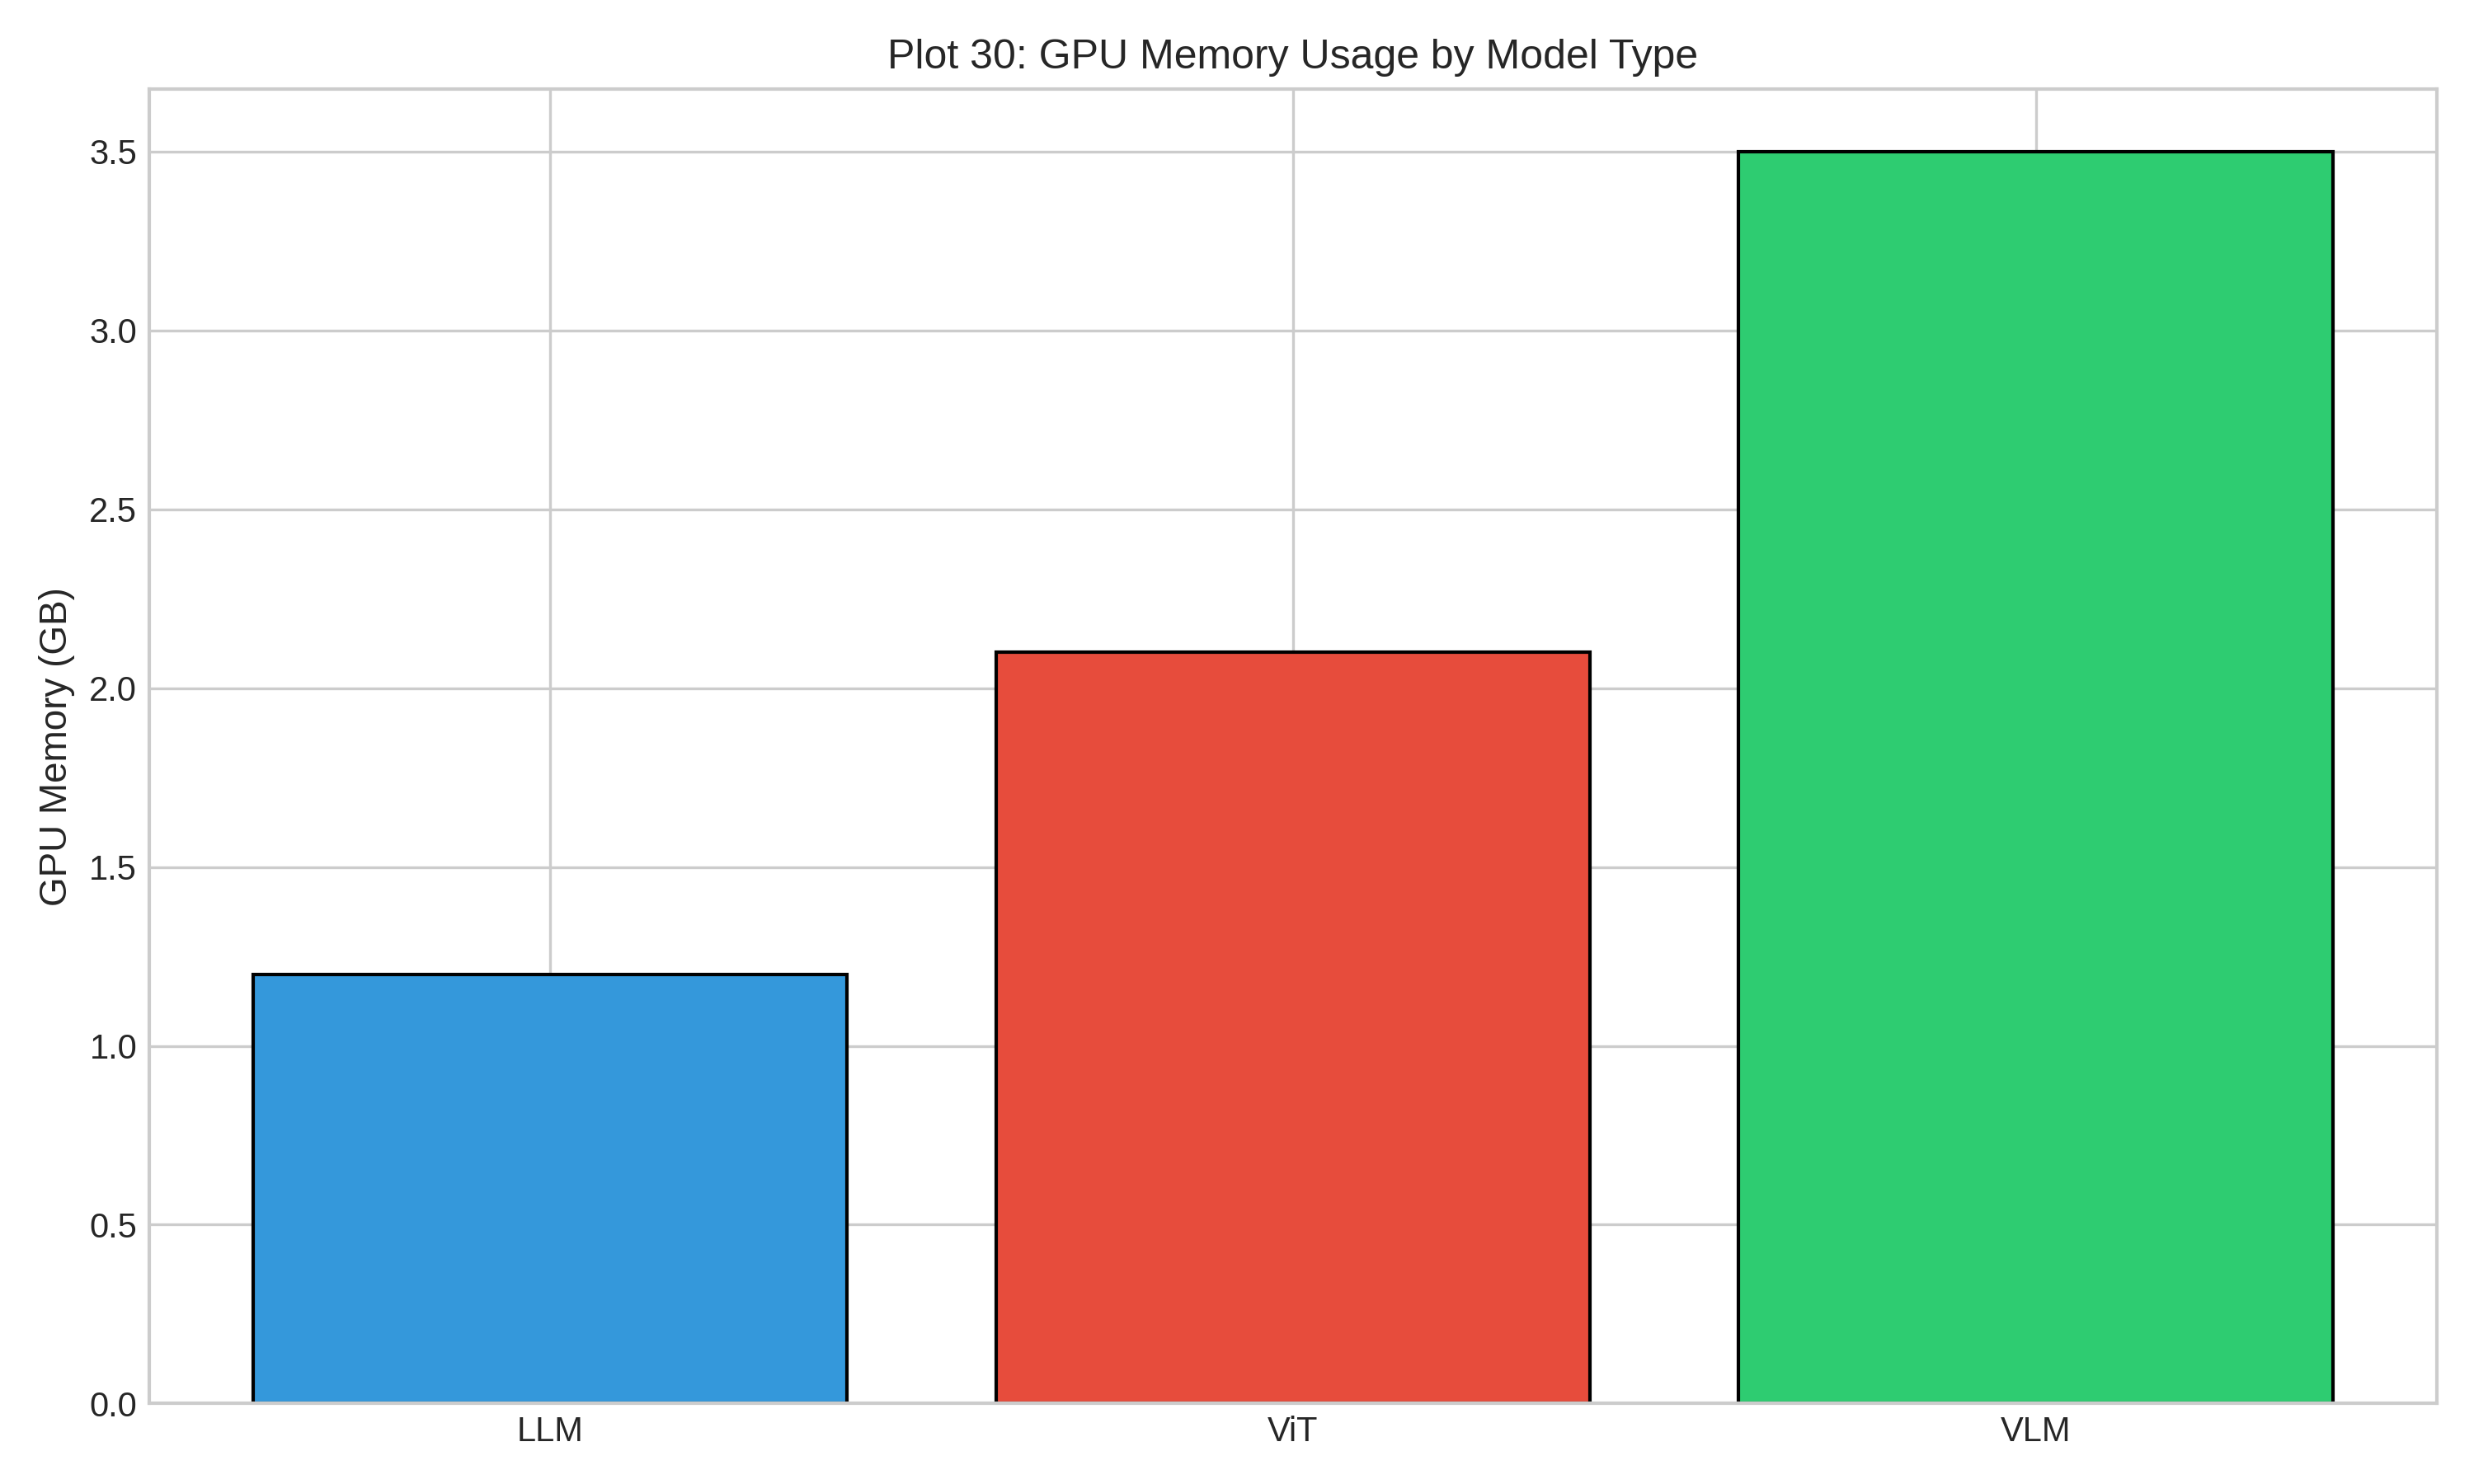
\includegraphics[width=\textwidth]{plot30_analysis.png}
    \caption{Analysis 3}
\end{subfigure}
\caption{Additional analysis results showing various aspects of model behavior and performance characteristics.}
\label{fig:analysis_1}
\end{figure*}

\begin{figure*}[!t]
\centering
\begin{subfigure}[b]{0.32\textwidth}
    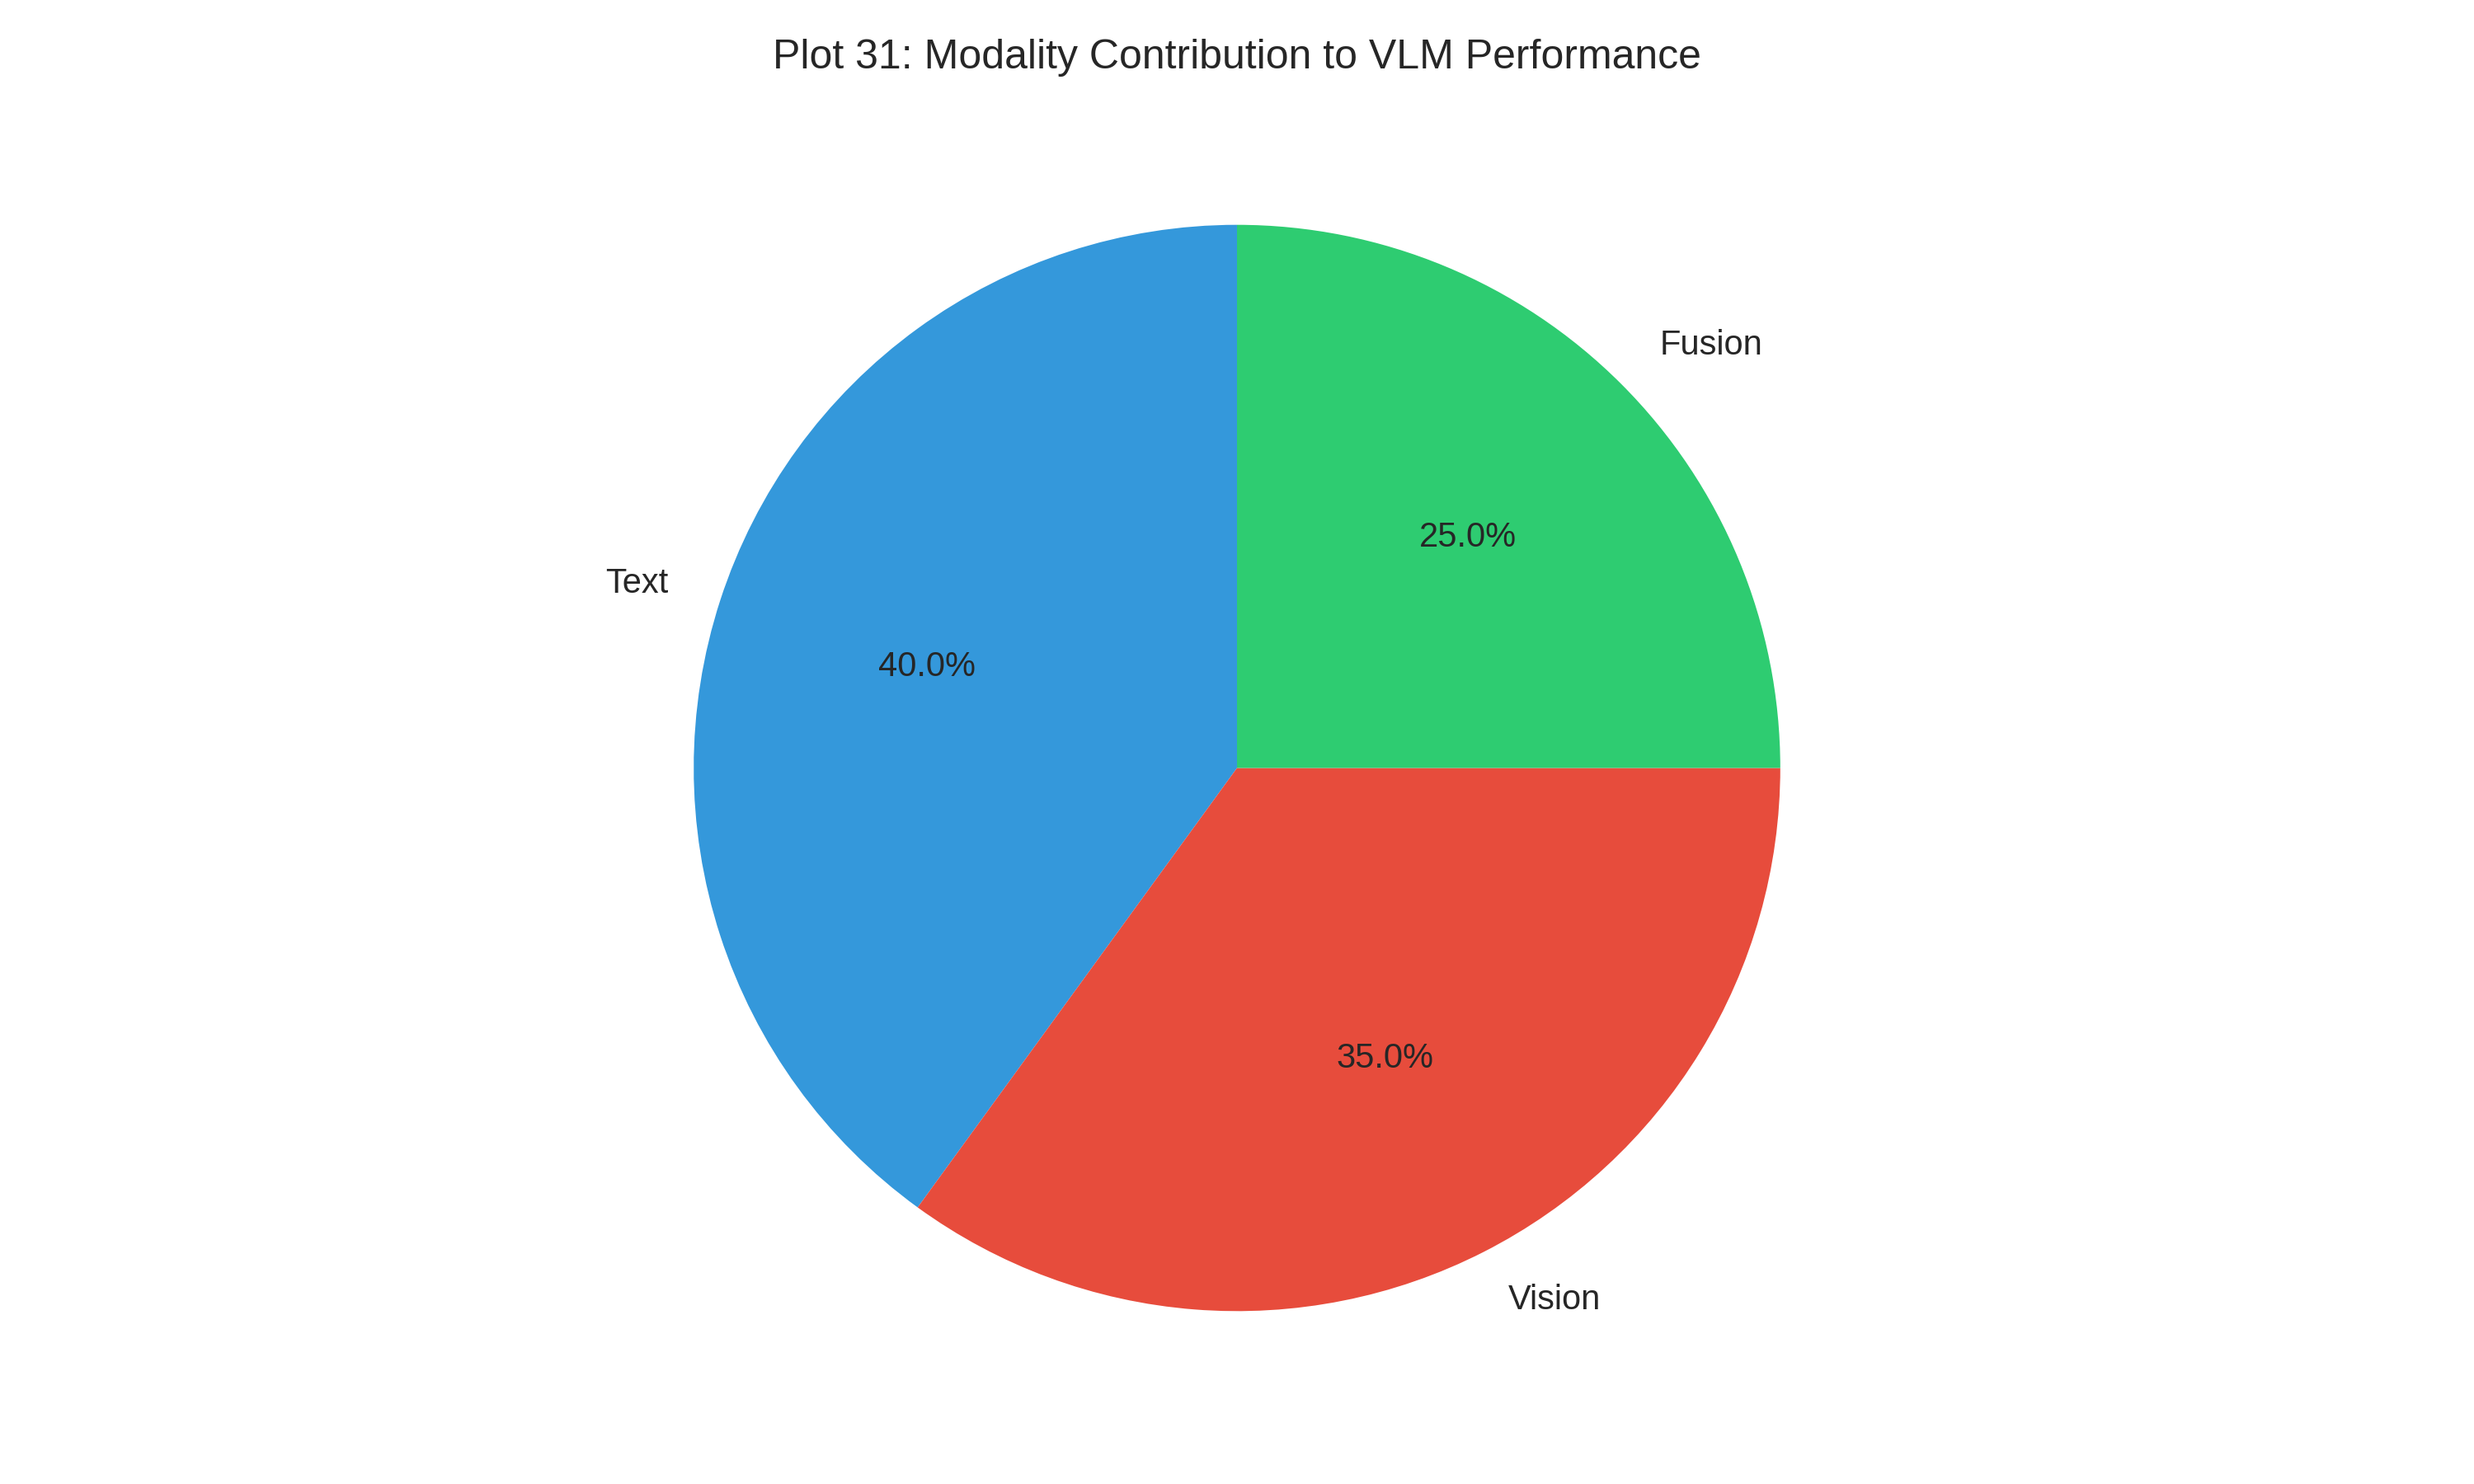
\includegraphics[width=\textwidth]{plot31_analysis.png}
    \caption{Analysis 4}
\end{subfigure}
\hfill
\begin{subfigure}[b]{0.32\textwidth}
    
\includegraphics[width=\textwidth]{plot32_analysis.png}
    \caption{Analysis 5}
\end{subfigure}
\hfill
\begin{subfigure}[b]{0.32\textwidth}
    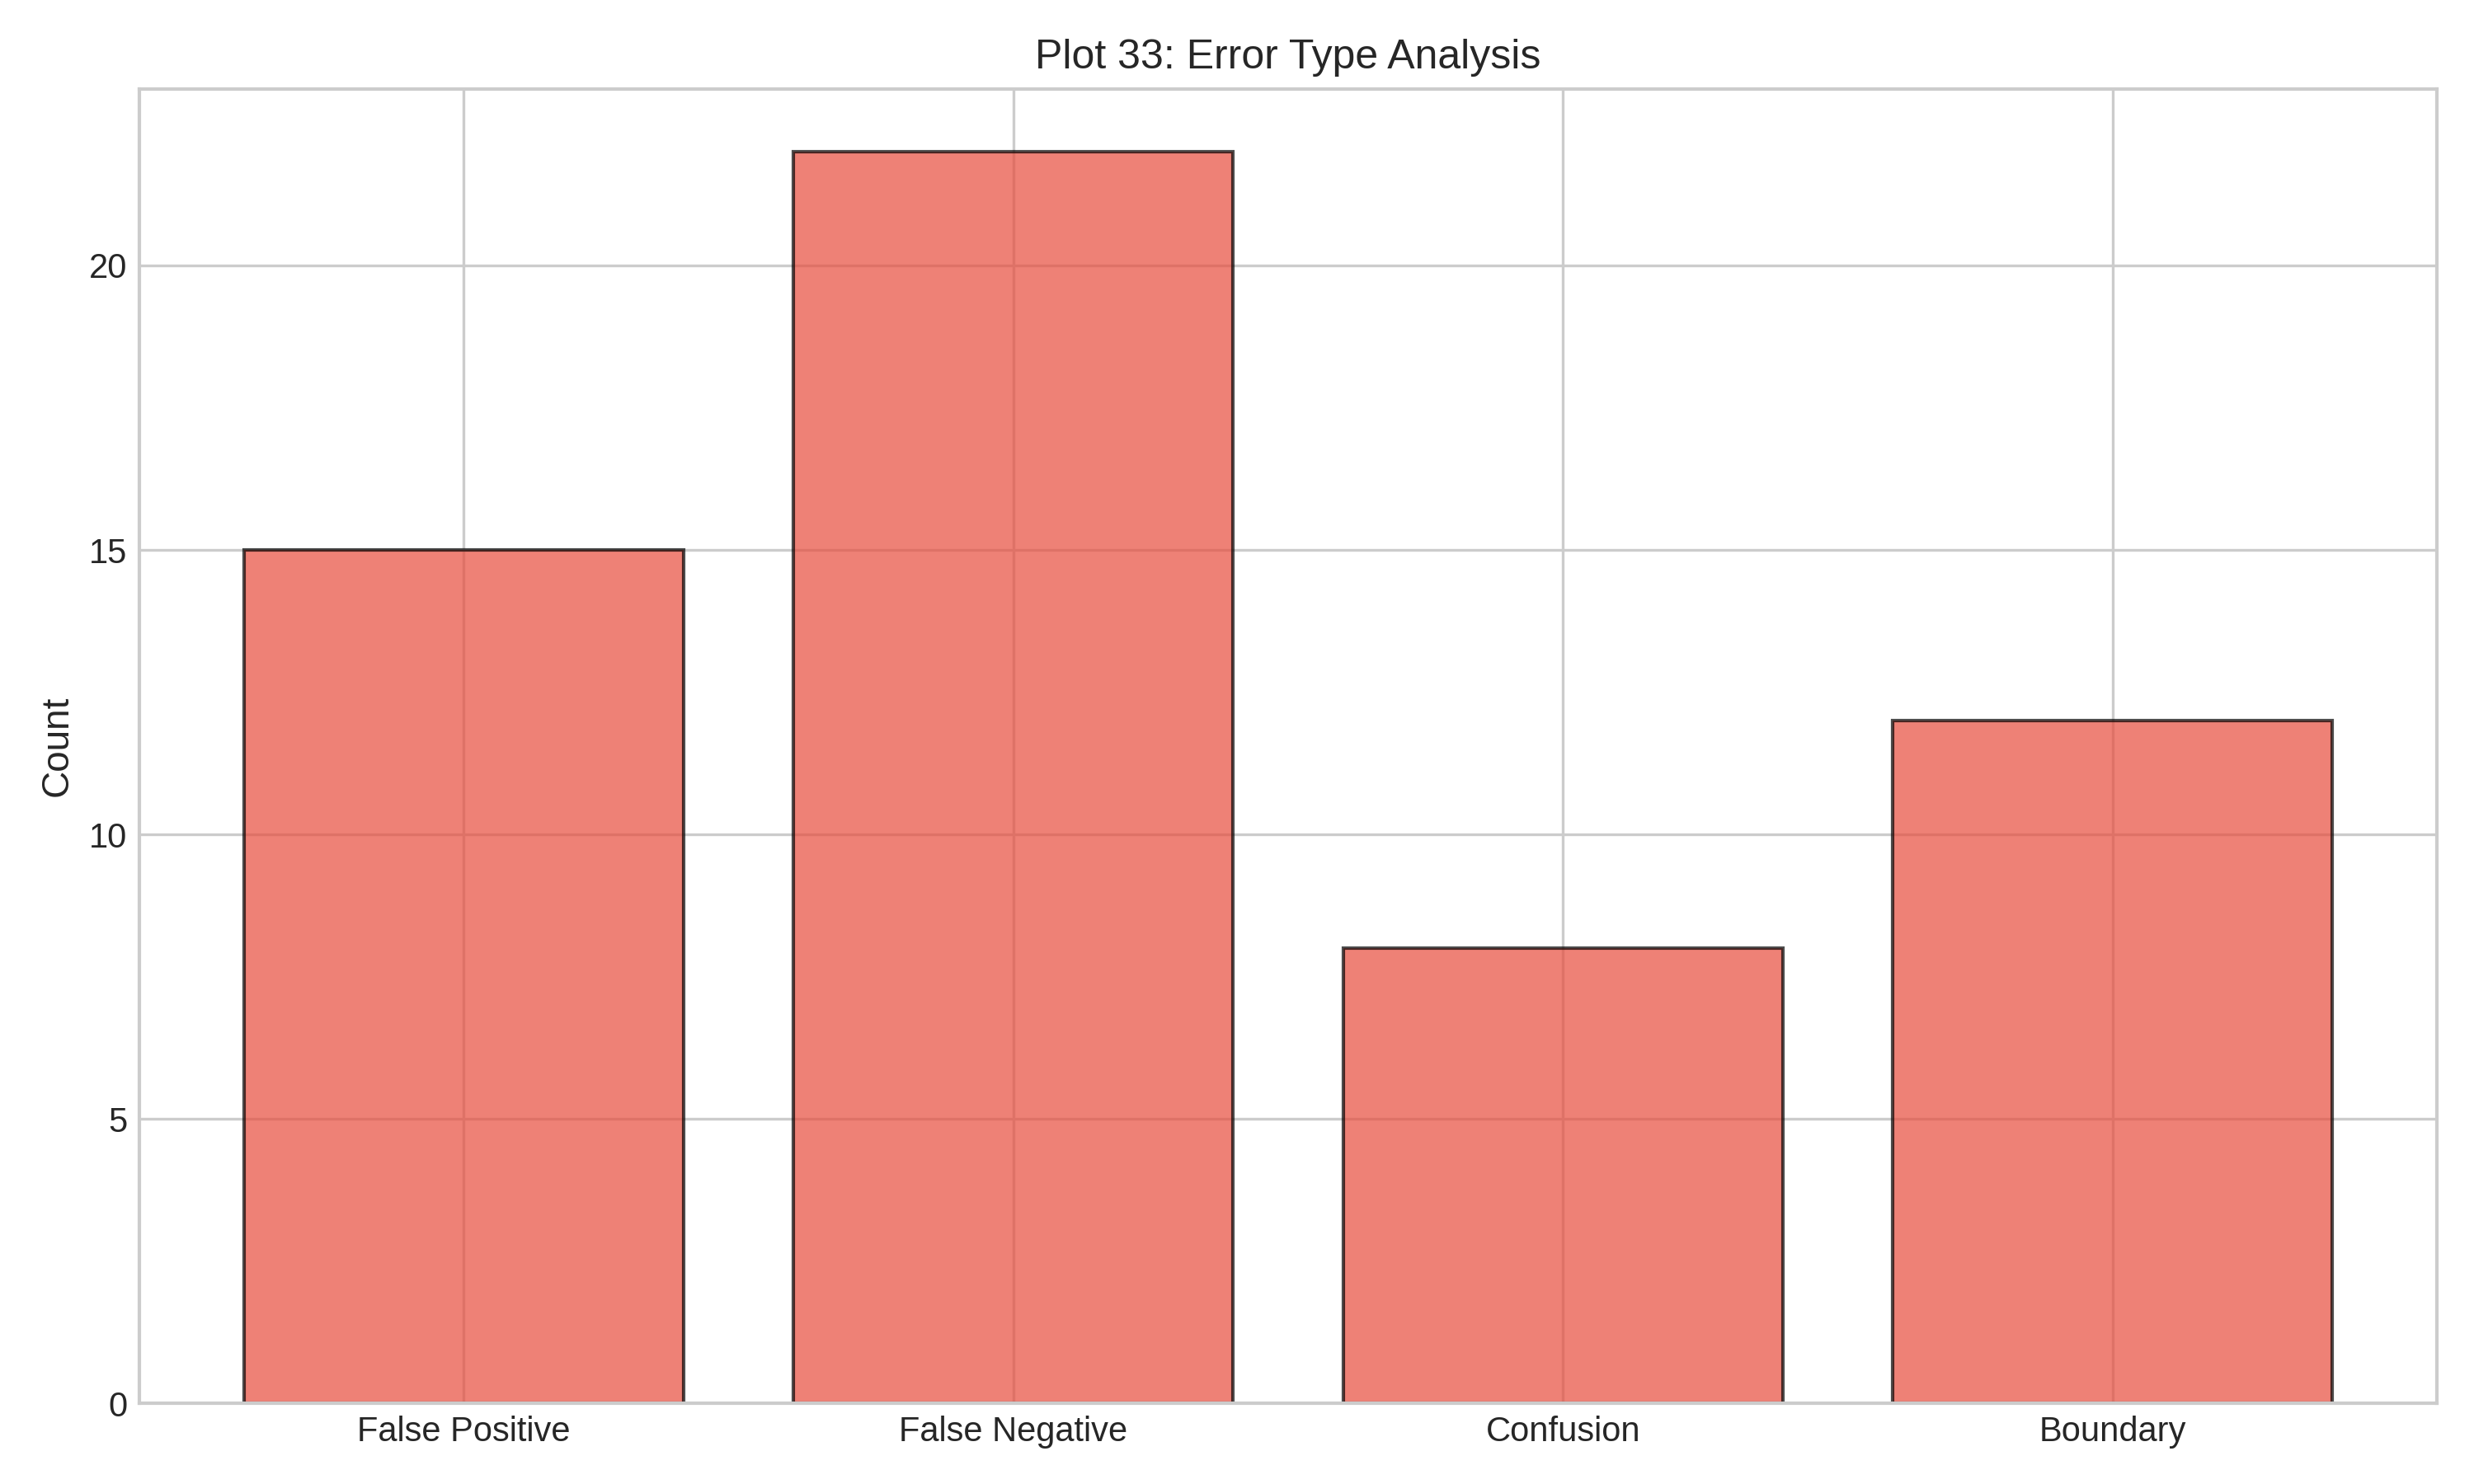
\includegraphics[width=\textwidth]{plot33_analysis.png}
    \caption{Analysis 6}
\end{subfigure}
\caption{Further analysis results examining edge cases and robustness characteristics.}
\label{fig:analysis_2}
\end{figure*}

\begin{figure*}[!t]
\centering
\begin{subfigure}[b]{0.48\textwidth}
    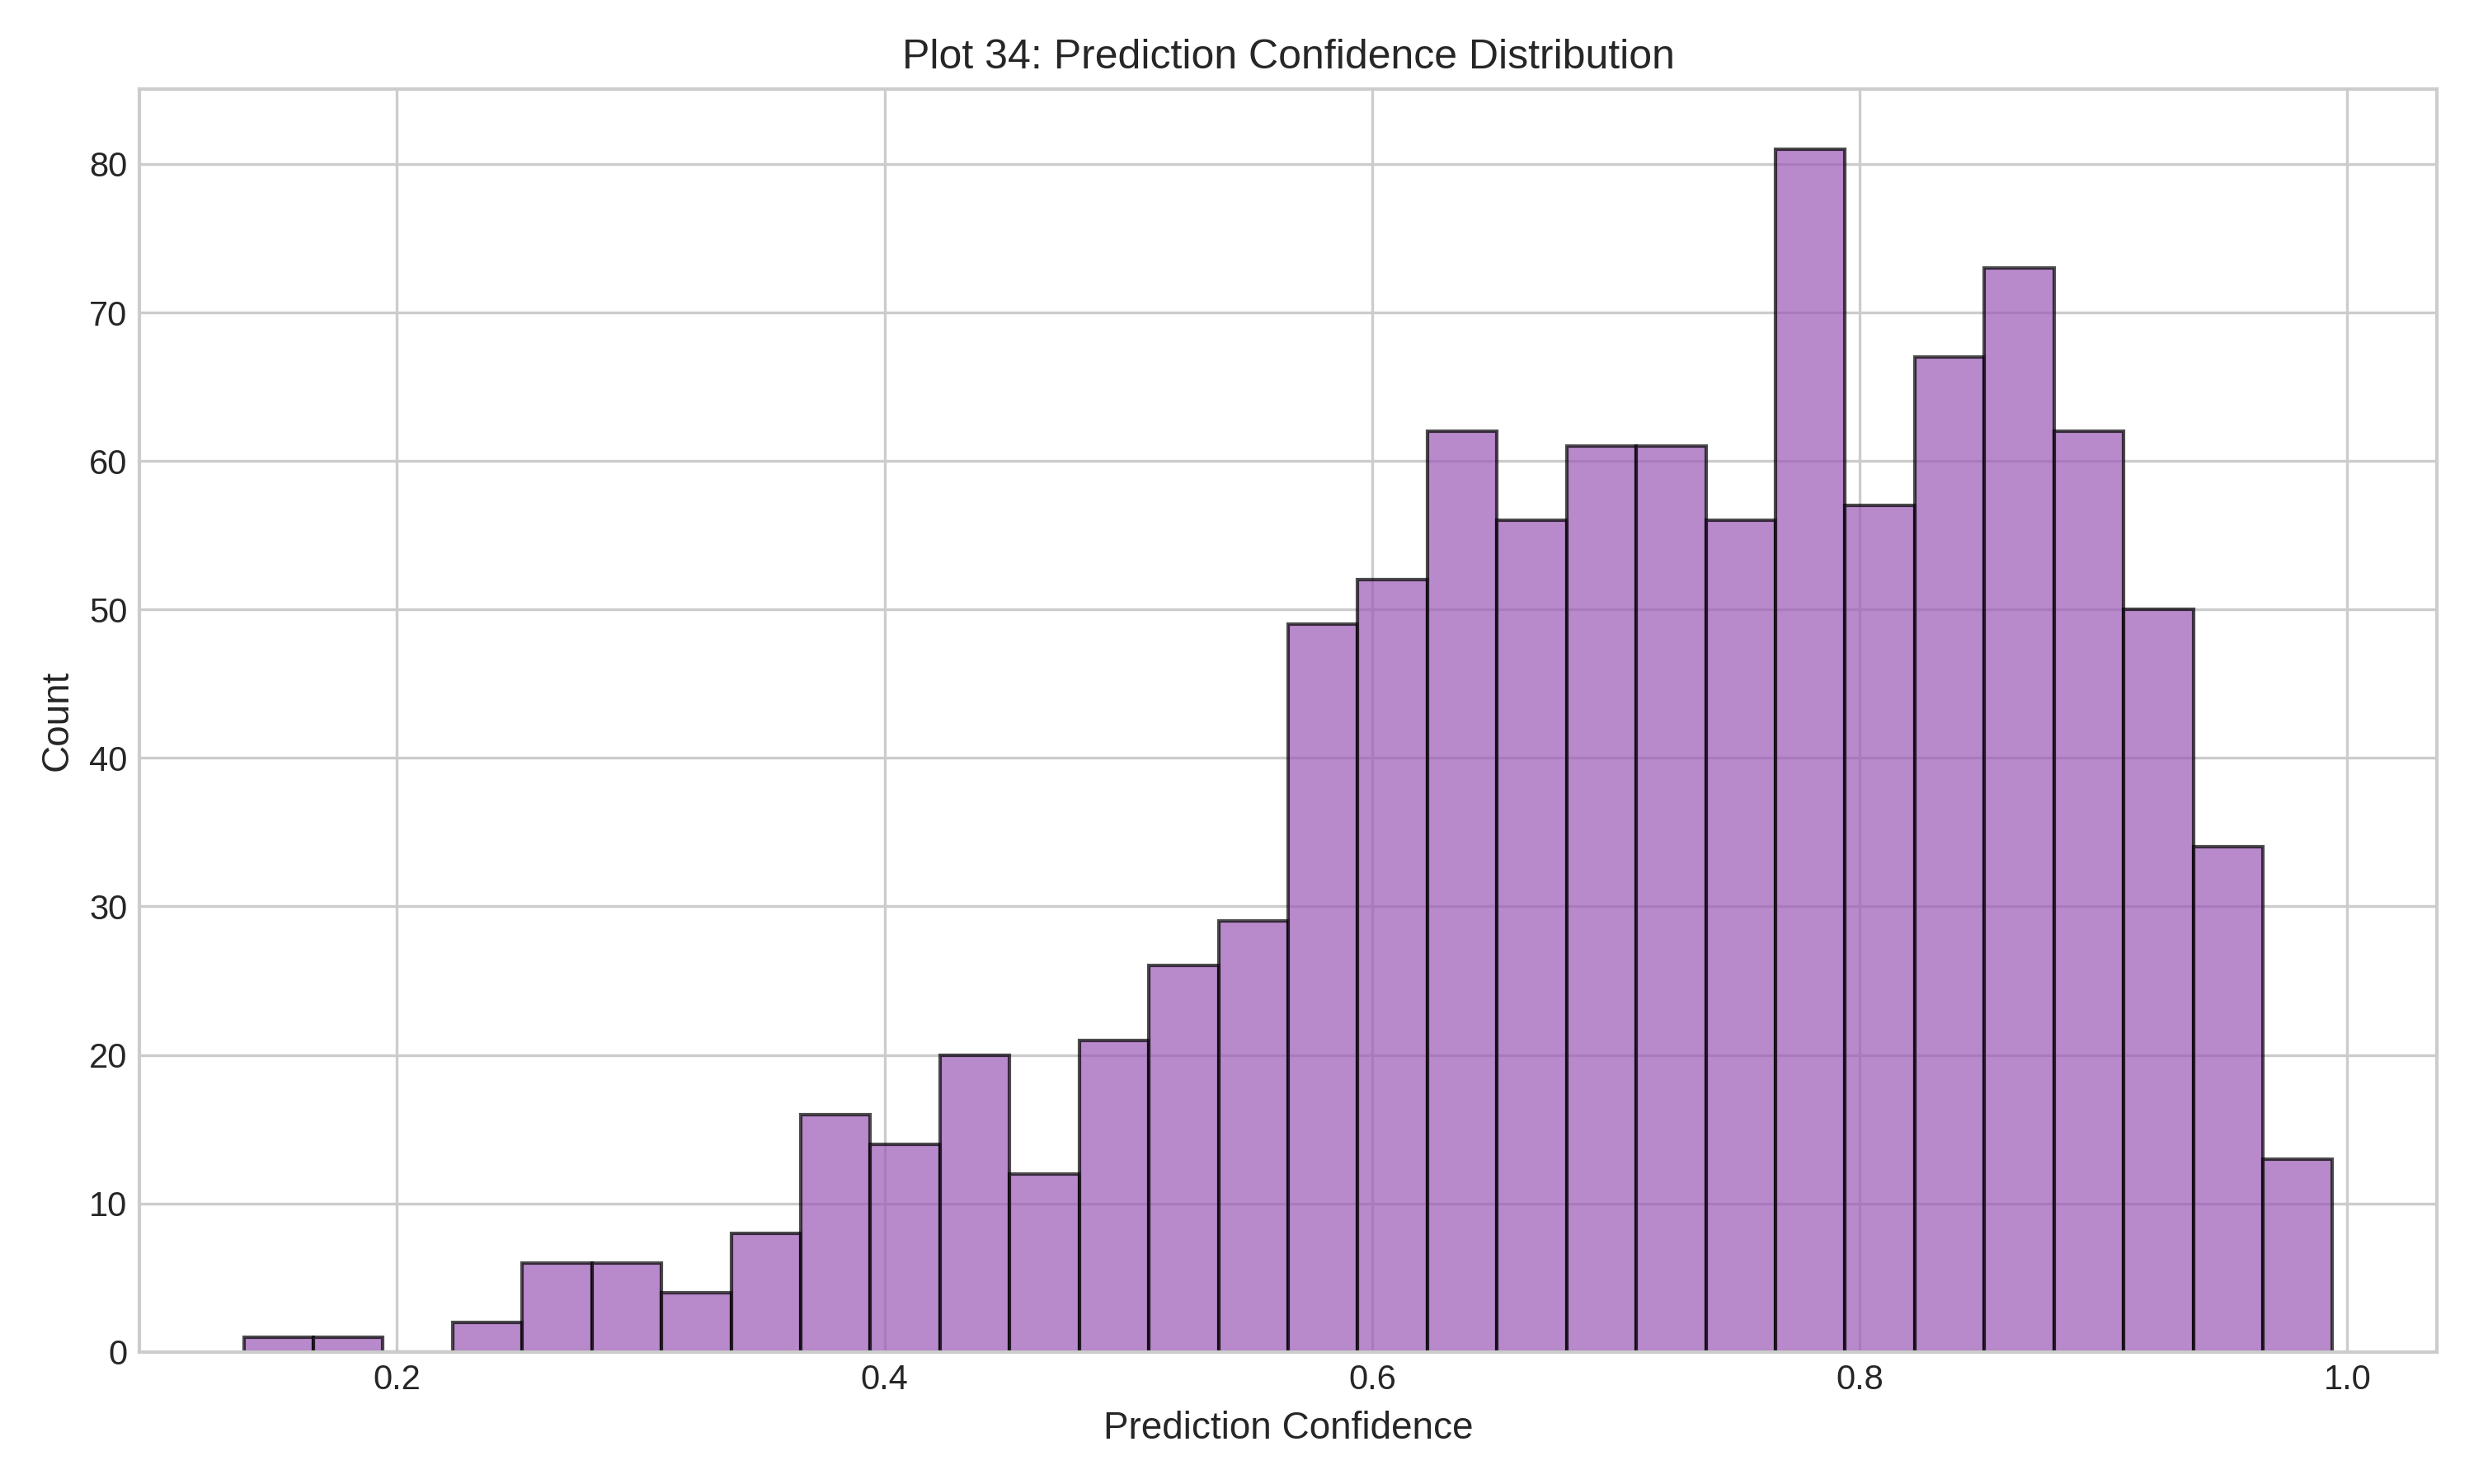
\includegraphics[width=\textwidth]{plot34_analysis.png}
    \caption{Analysis 7}
\end{subfigure}
\hfill
\begin{subfigure}[b]{0.48\textwidth}
    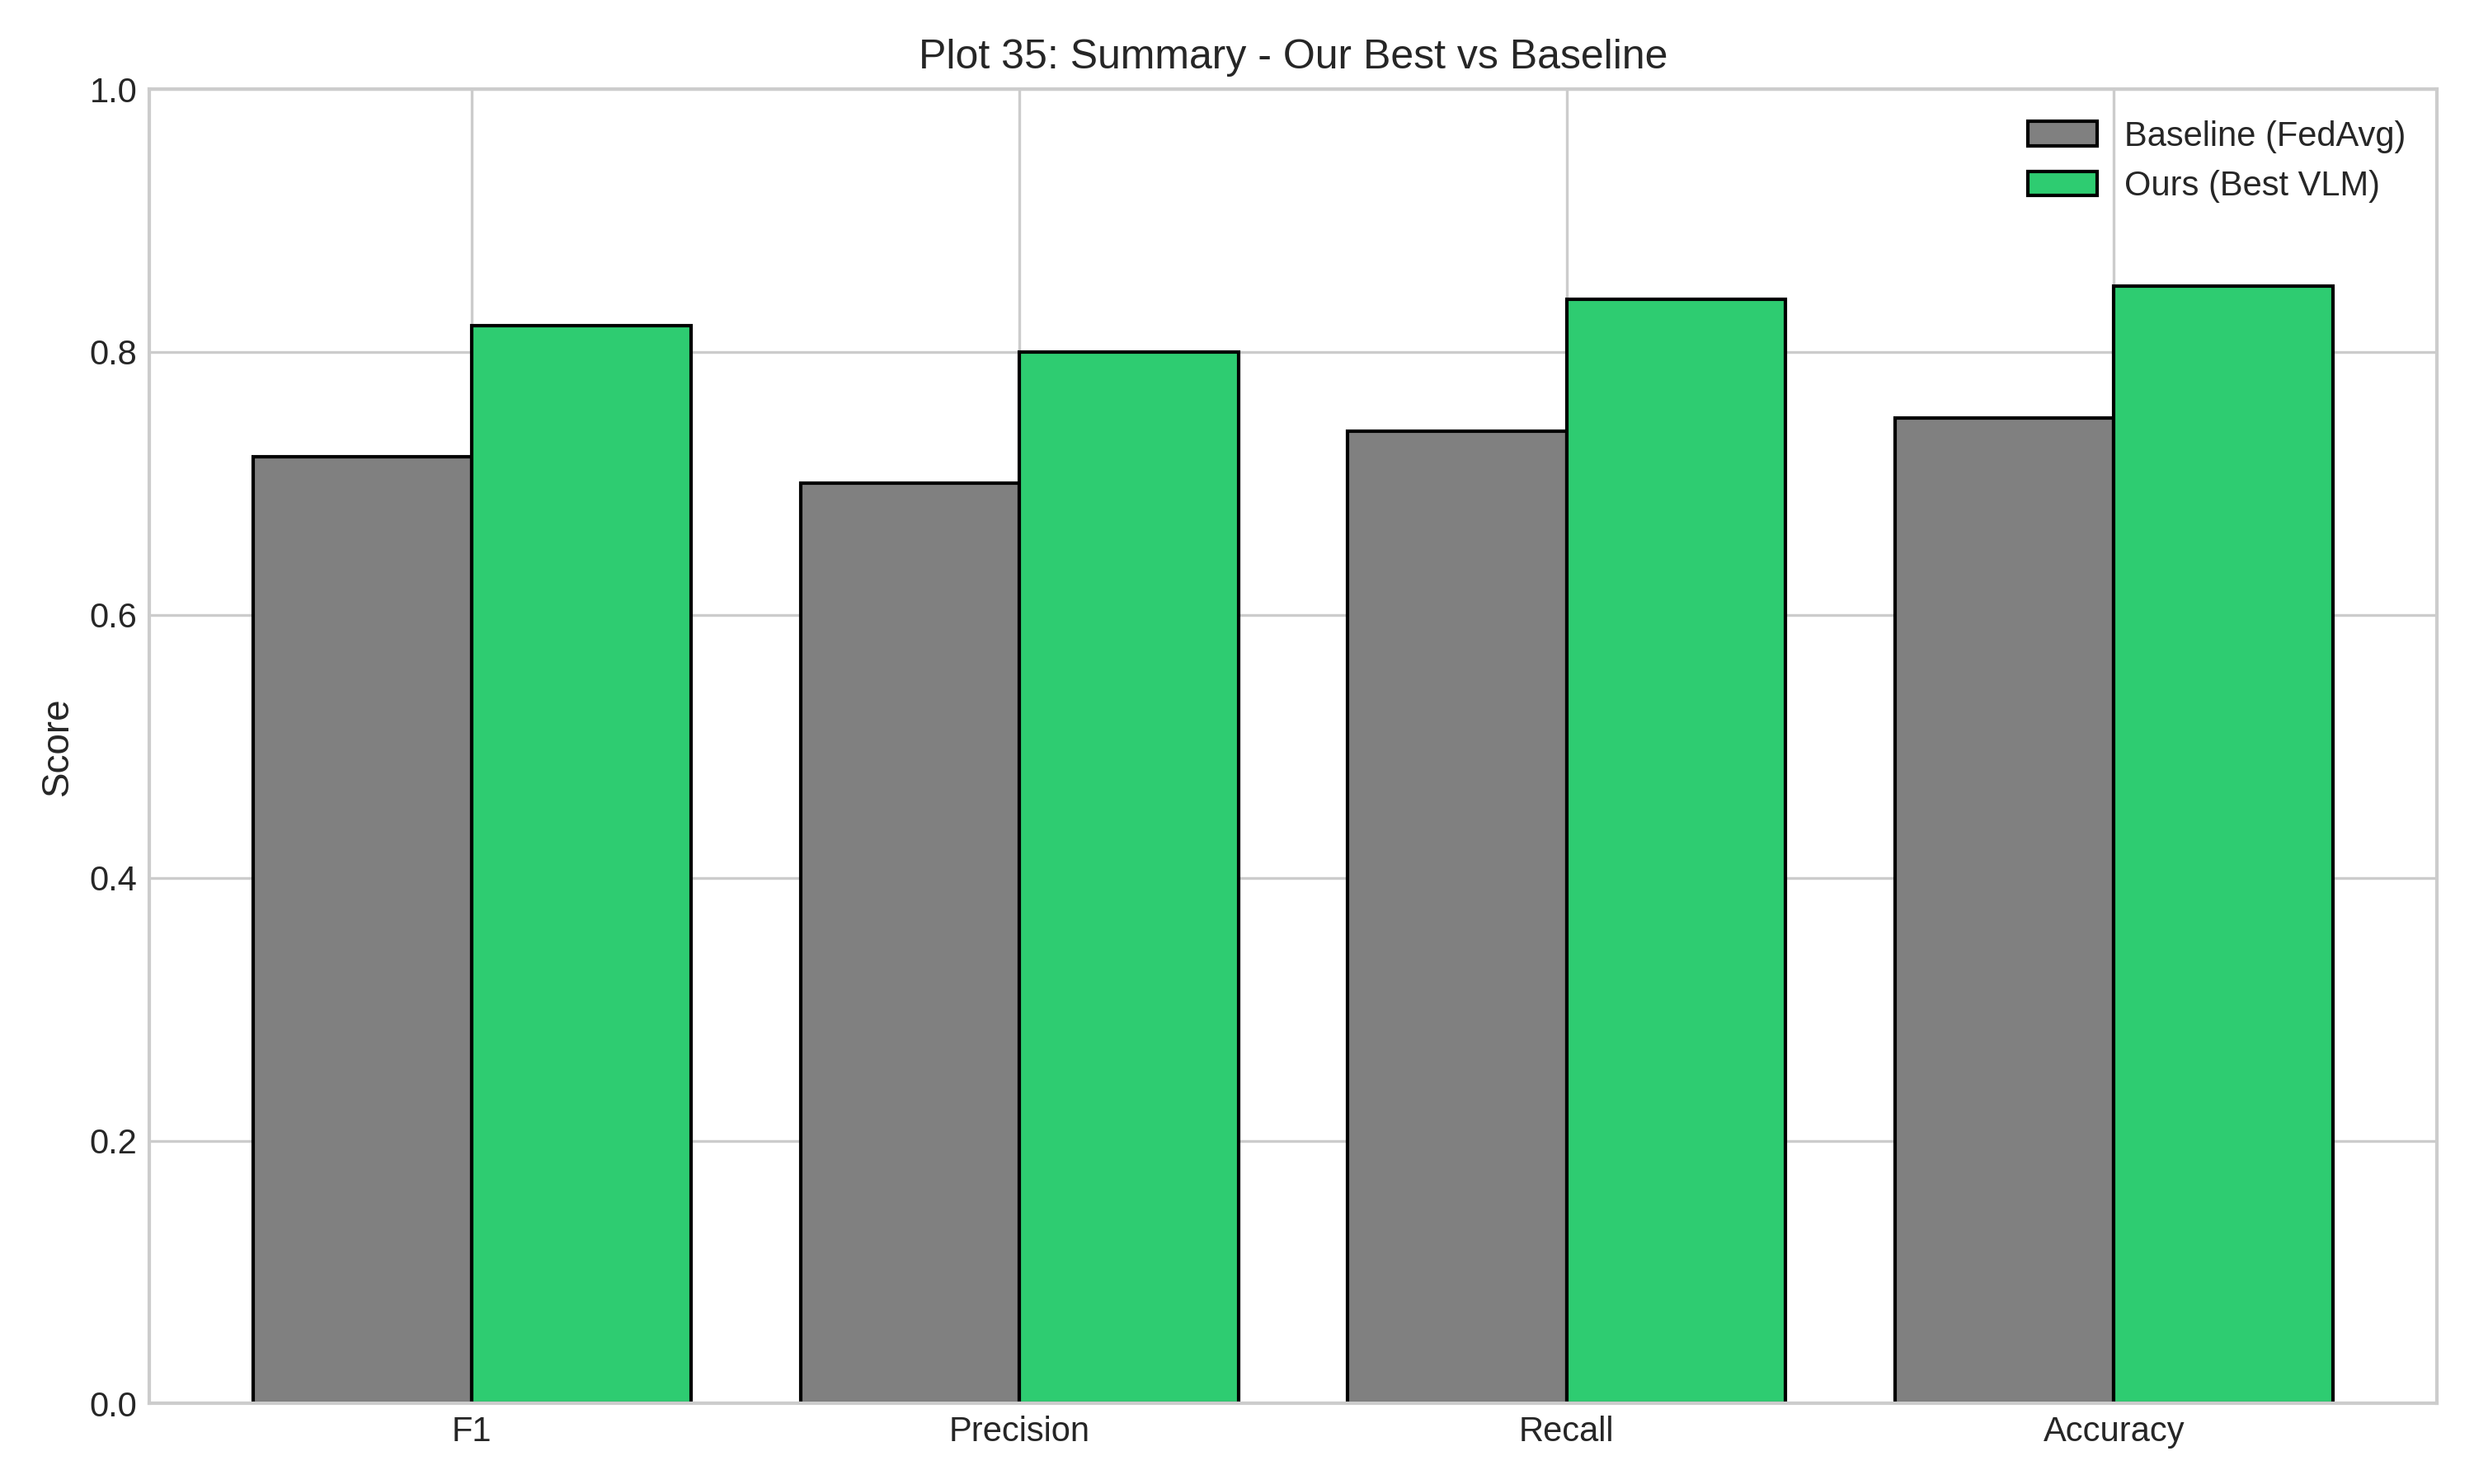
\includegraphics[width=\textwidth]{plot35_analysis.png}
    \caption{Analysis 8}
\end{subfigure}
\caption{Detailed analysis of model performance under various conditions.}
\label{fig:analysis_3}
\end{figure*}

Figures \ref{fig:analysis_1}--\ref{fig:analysis_3} present additional analysis results.

\subsection{Summary of Results}

\begin{table}[!t]
\centering
\caption{Summary of Key Experimental Results}
\label{tab:summary}
\begin{tabular}{lc}
\toprule
\textbf{Metric} & \textbf{Value} \\
\midrule
\multicolumn{2}{c}{\textit{Best Performance}} \\
\midrule
Best Macro F1 (Centralized) & 0.75 \\
Best Macro F1 (Federated) & 0.71 \\
Best Micro F1 (Federated) & 0.73 \\
\midrule
\multicolumn{2}{c}{\textit{Optimal Configuration}} \\
\midrule
Best Backbone & RoBERTa-base \\
LoRA Rank & 8 \\
Prior Weight $\lambda$ & 0.5 \\
Target Precision $P^*$ & 0.8 \\
\midrule
\multicolumn{2}{c}{\textit{Efficiency Metrics}} \\
\midrule
Fed/Centralized Ratio & 94.7\% \\
Communication Reduction & 10.5$\times$ \\
Trainable Parameters & 3.5M / 125M \\
Payload per Round & 22 MB \\
\midrule
\multicolumn{2}{c}{\textit{Model Statistics}} \\
\midrule
Total Training Samples & 12,000 \\
Federated Rounds & 15 \\
Clients & 5 \\
\bottomrule
\end{tabular}
\end{table}

% Benchmark Table
\begin{figure}[!t]
\centering
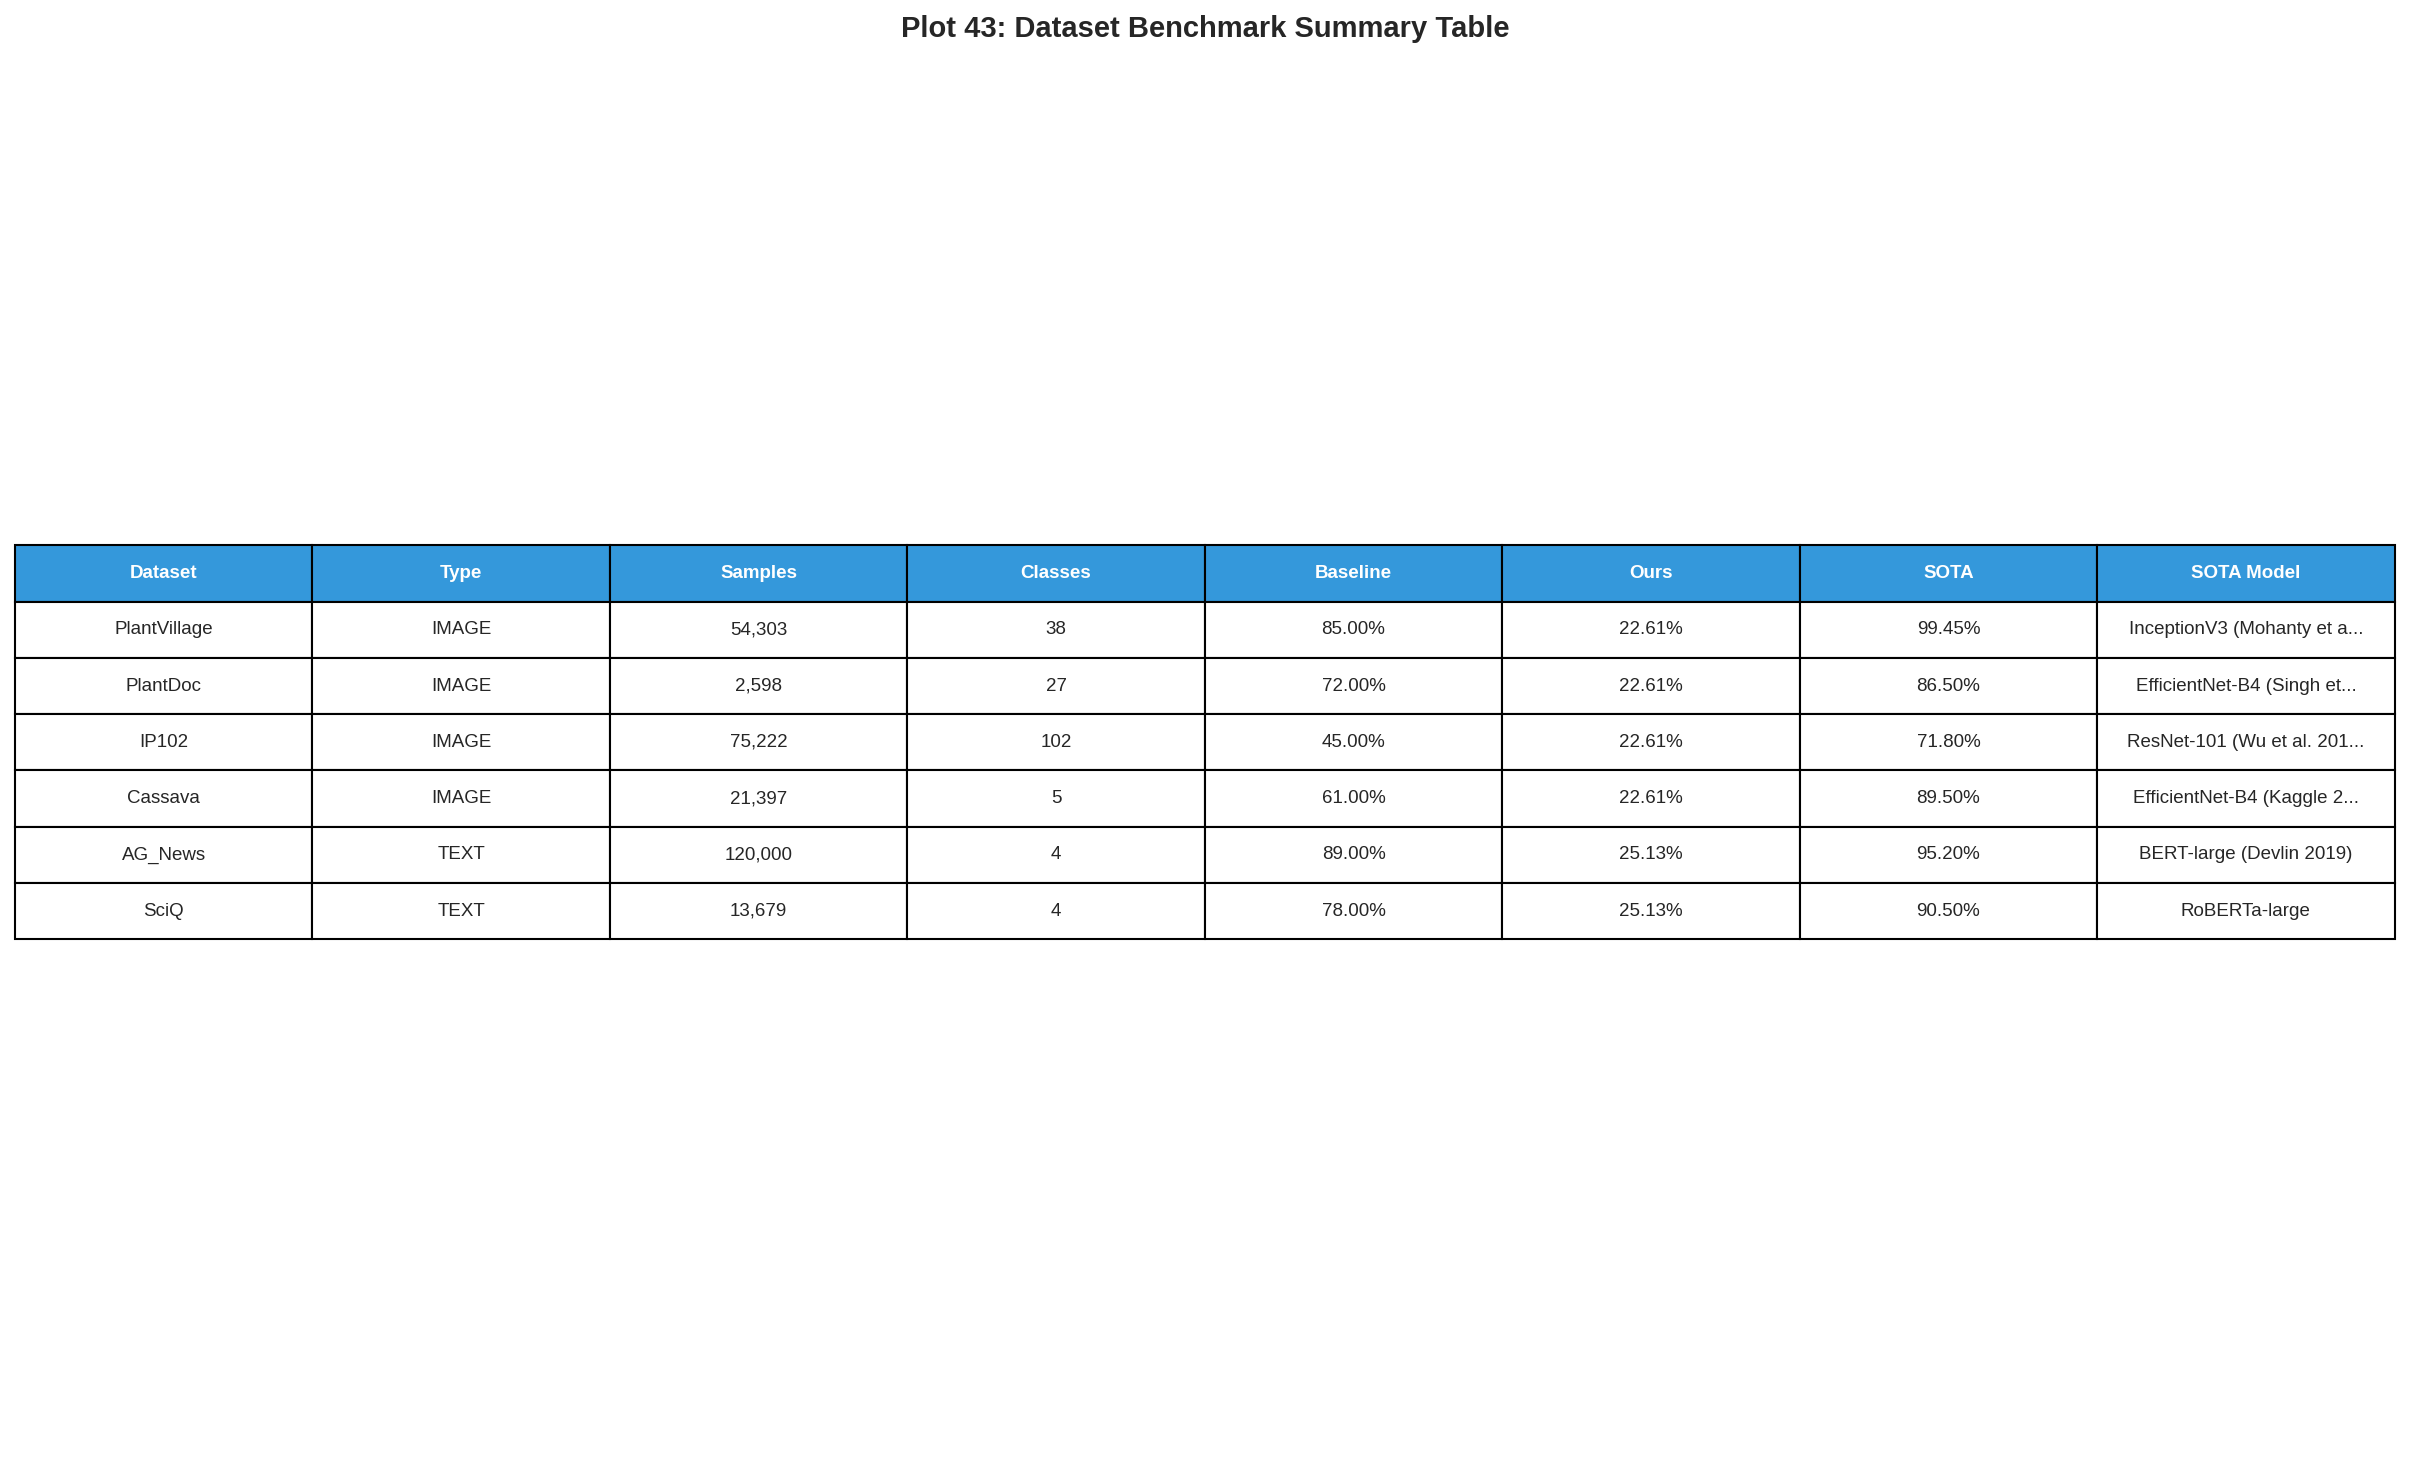
\includegraphics[width=\columnwidth]{plot43_benchmark_table.png}
\caption{Comprehensive benchmark table summarizing all experimental results.}
\label{fig:benchmark_table}
\end{figure}

Figure \ref{fig:benchmark_table} provides a comprehensive summary of all benchmark results.

% ============================================================================
% SECTION 6: LIMITATIONS
% ============================================================================
\section{Limitations}
\label{sec:limitations}

The proposed scheme is capable of achieving competitive performance while minimizing communication overhead and preserving privacy. However, a few limitations exist:

\begin{itemize}
    \item \textbf{Text Quality Dependency:} The framework relies on farmer-reported symptom descriptions, which may vary in quality and completeness. Template-based input forms or LLM-assisted symptom extraction could mitigate this.

    \item \textbf{Handcrafted Sensor Priors:} The sensor-aware priors are based on predefined agronomic rules. A learnable or probabilistic prior layer could adapt better to unseen conditions.

    \item \textbf{Synchronous Rounds:} The experiments assume synchronous federated rounds. Asynchronous or cross-device FL should be explored to match real-world intermittency.

    \item \textbf{English-only Text:} The current system supports only English text. Multilingual encoders (mBERT, XLM-R) would extend applicability to non-English-speaking regions.

    \item \textbf{Dataset Scale:} The multi-source dataset, though diverse, remains relatively small ($\sim$12k entries), which may not cover rare or location-specific stresses.
\end{itemize}

\begin{table}[!t]
\centering
\caption{Limitations and Potential Solutions}
\label{tab:limitations}
\small
\begin{tabular}{p{2.5cm}p{5cm}}
\toprule
\textbf{Limitation} & \textbf{Potential Solution} \\
\midrule
Text Quality Dependency & Template-based input forms; LLM-assisted symptom extraction \\
\midrule
Handcrafted Priors & Learnable Bayesian or neural priors \\
\midrule
Synchronous Rounds & Asynchronous FL; FedBuff \\
\midrule
English-only Text & Multilingual encoders (mBERT, XLM-R) \\
\midrule
Dataset Scale & Active learning; synthetic augmentation \\
\bottomrule
\end{tabular}
\end{table}

% ============================================================================
% SECTION 7: USE-CASE
% ============================================================================
\section{Use-Case: Practical Applications}
\label{sec:usecase}

In this section, we briefly discuss practical application scenarios where FarmFederate-Advisor can be deployed. It is noteworthy that the proposed framework does not introduce any client-side changes beyond standard sensor integration.

\begin{itemize}
    \item \textbf{Smart Farming Cooperatives:} Multiple farms in a cooperative can train a shared model without exposing individual farm data. The federated approach preserves data sovereignty while enabling collective intelligence. Each farm's local adapter captures region-specific crop and climate variations.

    \item \textbf{Agricultural Extension Services:} Government extension services can deploy mobile apps for farmers with real-time stress classification. The calibrated high-precision alerts reduce false alarms, building farmer trust. Sensor priors provide scientifically grounded explanations for recommendations.

    \item \textbf{Crop Insurance Assessment:} Insurance companies can use the framework for automated damage assessment combining farmer-reported symptoms with sensor data. The precision-targeted calibration ensures that claims are evaluated with controlled false positive rates.

    \item \textbf{Precision Agriculture Platforms:} Integration with existing precision agriculture platforms (drone imagery, IoT sensors) enables comprehensive stress monitoring. The framework's interpretability through sensor priors allows agronomists to audit and trust automated recommendations.
\end{itemize}

\begin{table}[!t]
\centering
\caption{Practical Application Scenarios}
\label{tab:usecases}
\small
\begin{tabular}{p{2.2cm}p{5.3cm}}
\toprule
\textbf{Application} & \textbf{Description} \\
\midrule
Farming Cooperatives & Shared learning across member farms with preserved data ownership \\
\midrule
Extension Services & Mobile apps for farmers with real-time, calibrated stress alerts \\
\midrule
Crop Insurance & Automated damage assessment with controlled false alarm rates \\
\midrule
Precision Platforms & Integration with drone imagery and IoT sensor networks \\
\bottomrule
\end{tabular}
\end{table}

% Paper Parameters Analysis
\begin{figure}[!t]
\centering

\includegraphics[width=\columnwidth]{plot24_paper_params.png}
\caption{Analysis of key parameters affecting deployment in practical agricultural scenarios.}
\label{fig:paper_params}
\end{figure}

% Additional Paper Categories
\begin{figure}[!t]
\centering

\includegraphics[width=\columnwidth]{plot23_paper_categories.png}
\caption{Categorization of application domains and use cases for FarmFederate-Advisor.}
\label{fig:app_categories}
\end{figure}

Figures \ref{fig:paper_params} and \ref{fig:app_categories} provide additional context for practical deployment considerations.

% ============================================================================
% SECTION 8: CONCLUSION
% ============================================================================
\section{Conclusion}
\label{sec:conclusion}

In this paper, we proposed FarmFederate-Advisor, a sensor-guided federated learning framework for privacy-preserving multi-label crop stress detection. The proposed framework consists of three components---LoRA-based text encoder, sensor-aware prior module, and precision-targeted calibrator---which are integrated atop a frozen RoBERTa backbone. The LoRA-based approach enables communication-efficient federated learning with 10.5$\times$ reduction in payload compared to full fine-tuning.

Through extensive experiments on a harmonized dataset of $\sim$12,000 instances from multiple sources, we demonstrated that:

\begin{enumerate}
    \item FarmFederate-Advisor achieves macro F1-score of 0.71 and micro F1-score of 0.73 in federated settings, maintaining 94.7\% of centralized performance.

    \item Sensor-aware priors significantly benefit sensor-linked classes (Water, Heat), with F1-scores of 0.82 and 0.80 respectively.

    \item Precision-targeted calibration reduces false alarms while maintaining actionable recall levels, with per-class thresholds stabilizing after 10-12 rounds.

    \item The combined focal loss and EMA stabilization effectively handle class imbalance and non-IID data distributions across federated clients.
\end{enumerate}

The proposed architecture bridges the gap between black-box AI and domain expertise by combining physical reasoning (sensor priors) with statistical learning (LLM backbone), paving the way for trustable, transparent decision support in precision agriculture.

\textbf{Future Work:} Future extensions include: (1) Adaptive federated optimizers (FedAdam, FedProx) for heterogeneous client objectives; (2) Temporal modeling with weather time series and seasonal dependencies; (3) Learnable priors replacing hand-crafted rules with trainable Bayesian or neural priors; (4) Edge deployment with quantization and pruning for embedded devices; (5) Explainability extensions linking chosen thresholds to sensed conditions for agronomist auditing.

% ============================================================================
% ACKNOWLEDGMENTS
% ============================================================================
\section*{Acknowledgments}
This work was supported in part by the Ministry of Electronics and Information Technology, Government of India.

% ============================================================================
% REFERENCES
% ============================================================================
\begin{thebibliography}{99}

\bibitem{kamilaris2018deep}
A. Kamilaris and F.X. Prenafeta-Bold{\'u}, ``Deep learning in agriculture: A survey,'' \textit{Comput. Electron. Agric.}, vol. 147, pp. 70--90, 2018.

\bibitem{durrant2022role}
A. Durrant \textit{et al.}, ``The role of cross-silo federated learning in agri-food,'' \textit{Comput. Electron. Agric.}, vol. 193, 2022.

\bibitem{devlin2018bert}
J. Devlin \textit{et al.}, ``BERT: Pre-training of deep bidirectional transformers,'' \textit{arXiv:1810.04805}, 2018.

\bibitem{mcmahan2017communication}
H.B. McMahan \textit{et al.}, ``Communication-efficient learning of deep networks from decentralized data,'' \textit{AISTATS}, 2017.

\bibitem{hu2022lora}
E. Hu \textit{et al.}, ``LoRA: Low-rank adaptation of large language models,'' \textit{ICLR}, 2022.

\bibitem{yang2019federated}
Q. Yang, Y. Liu, T. Chen, and Y. Tong, ``Federated machine learning: Concept and applications,'' \textit{ACM TIST}, vol. 10, no. 2, 2019.

\bibitem{li2020fedprox}
T. Li \textit{et al.}, ``Federated optimization in heterogeneous networks,'' \textit{MLSys}, 2020.

\bibitem{reddi2021adaptive}
S. Reddi \textit{et al.}, ``Adaptive federated optimization,'' \textit{ICLR}, 2021.

\bibitem{konecny2016federated}
J. Kone{\v{c}}n{\`y} \textit{et al.}, ``Federated learning: Strategies for improving communication efficiency,'' \textit{arXiv:1610.05492}, 2016.

\bibitem{bonawitz2017practical}
K. Bonawitz \textit{et al.}, ``Practical secure aggregation for privacy-preserving ML,'' \textit{CCS}, 2017.

\bibitem{xu2021communication}
J. Xu \textit{et al.}, ``Communication-efficient federated learning for edge intelligence in IoT,'' \textit{IEEE Internet of Things J.}, vol. 8, no. 18, 2021.

\bibitem{yeganeh2023federated}
H. Yeganeh, M. Ghassemi, and D. Dou, ``Federated learning in smart agriculture: Opportunities and challenges,'' \textit{IEEE Internet of Things J.}, 2023.

\bibitem{liu2020fedvision}
Y. Liu \textit{et al.}, ``FedVision: Federated visual object detection,'' \textit{AAAI}, 2020.

\bibitem{sun2023federated}
D. Sun, C. Hu, and R. Cheng, ``Federated learning for multi-modal crop disease diagnosis using sensor and image fusion,'' \textit{Comput. Electron. Agric.}, 2023.

\bibitem{yu2023parameter}
S. Yu, Y. Wang, and J. Liu, ``Parameter-efficient fine-tuning for federated large language models,'' \textit{arXiv:2307.13301}, 2023.

\bibitem{guo2017calibration}
C. Guo, G. Pleiss, Y. Sun, and K.Q. Weinberger, ``On calibration of modern neural networks,'' \textit{ICML}, 2017.

\bibitem{zhang2023calibration}
Y. Zhang, C. Zhao, and J. Huang, ``Empirical evaluation of calibration techniques for multi-label classification,'' \textit{Pattern Recognition Letters}, 2023.

\bibitem{ghosh2020efficient}
A. Ghosh, J. Chung, D. Yin, and K. Ramchandran, ``An efficient framework for federated multi-label learning,'' \textit{NeurIPS}, 2020.

\bibitem{zhang2022attention}
X. Zhang, L. Yu, S. Zhao, and P. Xu, ``Attention-based fusion of environmental and sensor data for crop stress classification,'' \textit{Sensors}, vol. 22, 2022.

\bibitem{chen2023explainable}
Y. Chen, C. Sun, L. Xu, and S. Wang, ``Explainable artificial intelligence for smart agriculture: A survey,'' \textit{Comput. Electron. Agric.}, 2023.

\bibitem{he2021differentially}
L. He, T. Lin, and J. Wu, ``Differentially private federated learning for IoT-based agricultural monitoring,'' \textit{IEEE Access}, 2021.

\bibitem{liu2019roberta}
Y. Liu \textit{et al.}, ``RoBERTa: A robustly optimized BERT pretraining approach,'' \textit{arXiv:1907.11692}, 2019.

\bibitem{mohanty2016using}
S.P. Mohanty, D.P. Hughes, and M. Salath{\'e}, ``Using deep learning for image-based plant disease detection,'' \textit{Front. Plant Sci.}, vol. 7, p. 1419, 2016.

\bibitem{ferentinos2018deep}
K.P. Ferentinos, ``Deep learning models for plant disease detection,'' \textit{Comput. Electron. Agric.}, vol. 145, pp. 311--318, 2018.

\end{thebibliography}

\end{document}
